%%
%% This is file `thesis-ex.tex',
%% generated with the docstrip utility.
%%
%% The original source files were:
%%
%% uiucthesis2009.dtx  (with options: `example')
%% 
\def\fileversion{v2.25a} \def\filedate{2009/10/10}
%% Package and Class "uiucthesis2009" for use with LaTeX2e.
\documentclass[edeposit,fullpage]{uiucthesis2009}
\usepackage{amsmath}
\usepackage{graphicx}
\usepackage{mathrsfs}   %The amsmath package is included for \xrightarrow
%\usepackage{natbib}
%\usepackage {apacite}
\usepackage{hyperref}
\usepackage{xcolor}

\usepackage{wasysym}
\usepackage{textcomp}



\begin{document}

\title{Application of a model-based nonlinear attitude control for quadrotor UAVs}
\author{Mingyo Seo}
\department{Mechanical Engineering}
\schools{B.Eng., Tohoku University, 2014}
\msthesis
\advisor{Associate Professor Prof. Soon-Jo Chung, Professor Prof. Seth Hutchinson}
\degreeyear{2016}
\committee{Professor Seth Hutchinson\\ Associate Professor Soon-Jo Chung}
\maketitle

\frontmatter

%% Create an abstract that can also be used for the ProQuest abstract.
%% Note that ProQuest truncates their abstracts at 350 words.
\begin{abstract}

A quadrotor, a UAV equipped with four rotors, has an advantage of its maneuver, and has been used for various purposes. For this advantage, many researchers have studied a quadrotor's operation. An attitude control system for a quadrotor is one of the most important parts in order to improve the quadrotor's performance.

This thesis developed a quadrotor testbed and applied a model-based nonlinear attitude control, originally designed for a space craft, to the quadrotor. In order to implement a nonlinear attitude control system, the dynamic model of the quadrotor is studied and the quadrotor's physical properties are characterized based on the model. Then, stability and agility of the nonlinear attitude control are validated by both simulations and experiments and its performance is compared with one of an conventional PID attitude control.

Finally, this thesis proposes a computationally-efficient position estimator for the quadrotor's operation. The position estimator detects visual markers of an image from the camera, and computes the quadrotor's position. The position estimator was also evaluated by experiments.

\end{abstract}

%% Create a dedication in italics with no heading, centered vertically
%% on the page.
%\begin{dedication}
%To Father and Mother.
%\end{dedication}

%% Create an Acknowledgements page, many departments require you to
%% include funding support in this.
\chapter*{Acknowledgments}
The author wishes to express sincere gratitude to Prof. Soon-Jo Chung and Prof. Seth Hutchinson, for their advice and guidance throughout this work. The author gratefully acknowledges the contributions of Elias Waddington to the hardware setup and the experiments reported in Chapters 2 and 4. Chapter 5 was conducted as joint work with Lingyu Ma, and the author would like to express thanks to him for his insightful discussions. 
% Finally, especially thanks to my family, Nari Kim, Taito Nabeshima, Wookyum Kim, Daniel Cho, Shenyu Liu, JCT members, and CEA members for their support during the process of earning my Master's degree.
\color{blue}
Finally, special thanks go to his family, Nari Kim, Taito Nabeshima, Wookyum Kim, Daniel Cho, Shenyu Liu, JCT members, and CEA members for their support during the process of earning his Master's degree.
\color{black}

%% The thesis format requires the Table of Contents to come
%% before any other major sections, all of these sections after
%% the Table of Contents must be listed therein (i.e., use \chapter,
%% not \chapter*).  Common sections to have between the Table of
%% Contents and the main text are:
%%
%% List of Tables
%% List of Figures
%% List Symbols and/or Abbreviations
%% etc.

\tableofcontents
\listoftables
\listoffigures

%% Create a List of Abbreviations. The left column
%% is 1 inch wide and left-justified
%\chapter{List of Abbreviations}

%\begin{symbollist*}
%\item[CA] Caffeine Addict.
%\item[CD] Coffee Drinker.
%\end{symbollist*}

%% Create a List of Symbols. The left column
%% is 0.7 inch wide and centered
%\chapter{List of Symbols}

%\begin{symbollist}[0.7in]
%\item[$\tau$] Time taken to drink one cup of coffee.
%\item[$\mu$g] Micrograms (of caffeine, generally).
%\end{symbollist}

\mainmatter
\chapter{Introduction}
\section{Background}
An unmanned aerial vehicle (UAV) is defined as an autonomous aircraft that can fly without a human pilot on board \cite{icao16}. %"ICAO?s circular 328 AN/190 : Unmanned Aircraft Systems" (PDF). ICAO. Retrieved 3 February 2016.
A quadrotor is a UAV that consists of two pairs of counter-rotating rotors with fixed-pitch blades \cite{Hoffmann07}. %Quadrotor Helicopter Flight Dynamics and Control: Theory and Experiment?
With independent output of each motor, the quadrotor has full control of its orientation (roll, pitch, and yaw) and thrust. The quadrotor's translation motion is coupled with the quadrotor attitude and thrust since the thrust occurs in only the perpendicular direction of the quadrotor orientation; the direction of the translation is determined by the orientation, and the magnitude of the translation is determined by the thrust. Therefore, the quadrotor controls its translation by altering its attitude and has a capacity of both rotation and translation maneuvers. Due to the advantage, quadrotors have been used for various purposes and performed tasks in environments that are nearly impossible to reach as a human. As an example, Michael et al. developed an autonomous quadrotor to explore an earthquake-damaged building with multiple floors collaborating with a ground robot \cite{Michael02}. %Collaborative Mapping of an Earthquake-Damaged Building via Ground and Aerial Robots
Chambers et al. developed a quadrotor system that maps rivers with a self-supervised river classification system \cite{Chambers11}.
%Perception for a River Mapping Robot

A control system for quadrotors usually consists of position control (outer-loop) and attitude control (inner-loop). Position control maps input of translation motion into desired orientation and thrust. Attitude control computes desired torque corresponding to the desired and current attitude. However, because of factors like rotational effects on translation motion, and aerodynamic effects, the dynamic model of the quadrotor is highly non-linear. Therefore, there is a demand of advanced control system for the quadrotor's performance.

\section{Related Works}
For improvement of quadrotors' performance, various research on advanced control systems for a quadrotor have been conducted actively. Raffo et al. applied a nonlinear \({\mathscr{H}}_{\infty}\) control to attitude control and designed a backstepping control for path tracking of a quadrotor. The control system was evaluated by simulations \cite{Raffo08}. %Backstepping/Nonlinear H? Control for Path Tracking of a QuadRotor Unmanned Aerial Vehicle
Morgan et al. designed and implemented a dynamic-model-based nonlinear attitude control in the swarm assignment and trajectory optimization \cite{Morgan16}. %Swarm assignment and trajectory optimization using variable-swarm, distributed auction assignment and sequential convex programming
In the case of the application of adaptive control, Mallikarjunan et al. demonstrated an application of \({\mathscr{L}}_{1}\)  adaptive control for quadrotors' attitude control by experiments \cite{Mallikarjunan12}. %L1 Adaptive Controller for Attitude Control of Multirotors
Also, Diao et al. suggested a Lyapunov based nonlinear adaptive control for a quadrotor under uncertainties of mass, inertia, and aerodynamic damping coefficients, and evaluated the control by simulations \cite{Diao11}. %A Nonlinear Adaptive Control Approach for Quadrotor UAVs

On the other side, trajectories of a quadrotor is also studied by many researchers to improve its performance. 
Ritz et al. designed a method to compute a quardrotor's time-optimal trajectory between two given states, and evaluated the method by simulations \cite{Ritz11}.
%Quadrocopter Performance Benchmarking Using Optimal Control
Mellinger et al. developed an algorithm of a trajectory generator for a quadrotor's aggressive maneuvers, and validated the quadrotor's performance by experiments \cite{Mellinger12}.
% Trajectory generation and control for precise aggressive maneuvers with quadrotors
In addition, Dierksand and Jagannathan suggested a control scheme that uses control inputs computed by neural networks \cite{Dierks10}. %Output Feedback Control of a Quadrotor UAV Using Neural Networks

Here, we develop a model based attitude control system focused on addressing the nonlinearity of quadrotor dynamics in order to improve agility and stability.

\section{Motivation}

Due to high nonlinearities of quadrotor dynamics, application of advanced controllers is expected to improve performance of the quadrotor, compared with conventional controllers, such as PID and Linear-Quadratic Regulator. Studies of quadrotor dynamics are expected to increase the robustness of the control systems.

The Aerospace Robotics and Control Laboratory at the University of Illinois had developed quadrotor platforms based on Crazyflie 1.0 to validate performance of nonlinear controllers \cite{Morgan16}.  %Swarm assignment and trajectory optimization using variable-swarm, distributed auction assignment and sequential convex programming
Crazyflie is a open-source nano quadrotor system developed by Bitcraze \cite{bitcraze}. %https://www.bitcraze.io
A Crazyflie quadrotor is about 19 g weight and each leg is about 6 cm length. However, due to the quadrotor's physical constrains, such as its load limit and sensor errors, its application is limited. Especially, in order to develop a vision-based position control system and other high-level functions for the quadrotor, only 8 g of load is allowed for sensors, equipments, and mount for them, and therefore, choice of sensors and algorithms is limited. A Crazyflie quadcopter with a camera and mount is shown in Figure \ref{fig:crazyflie}.

\begin{figure}
    \centering
    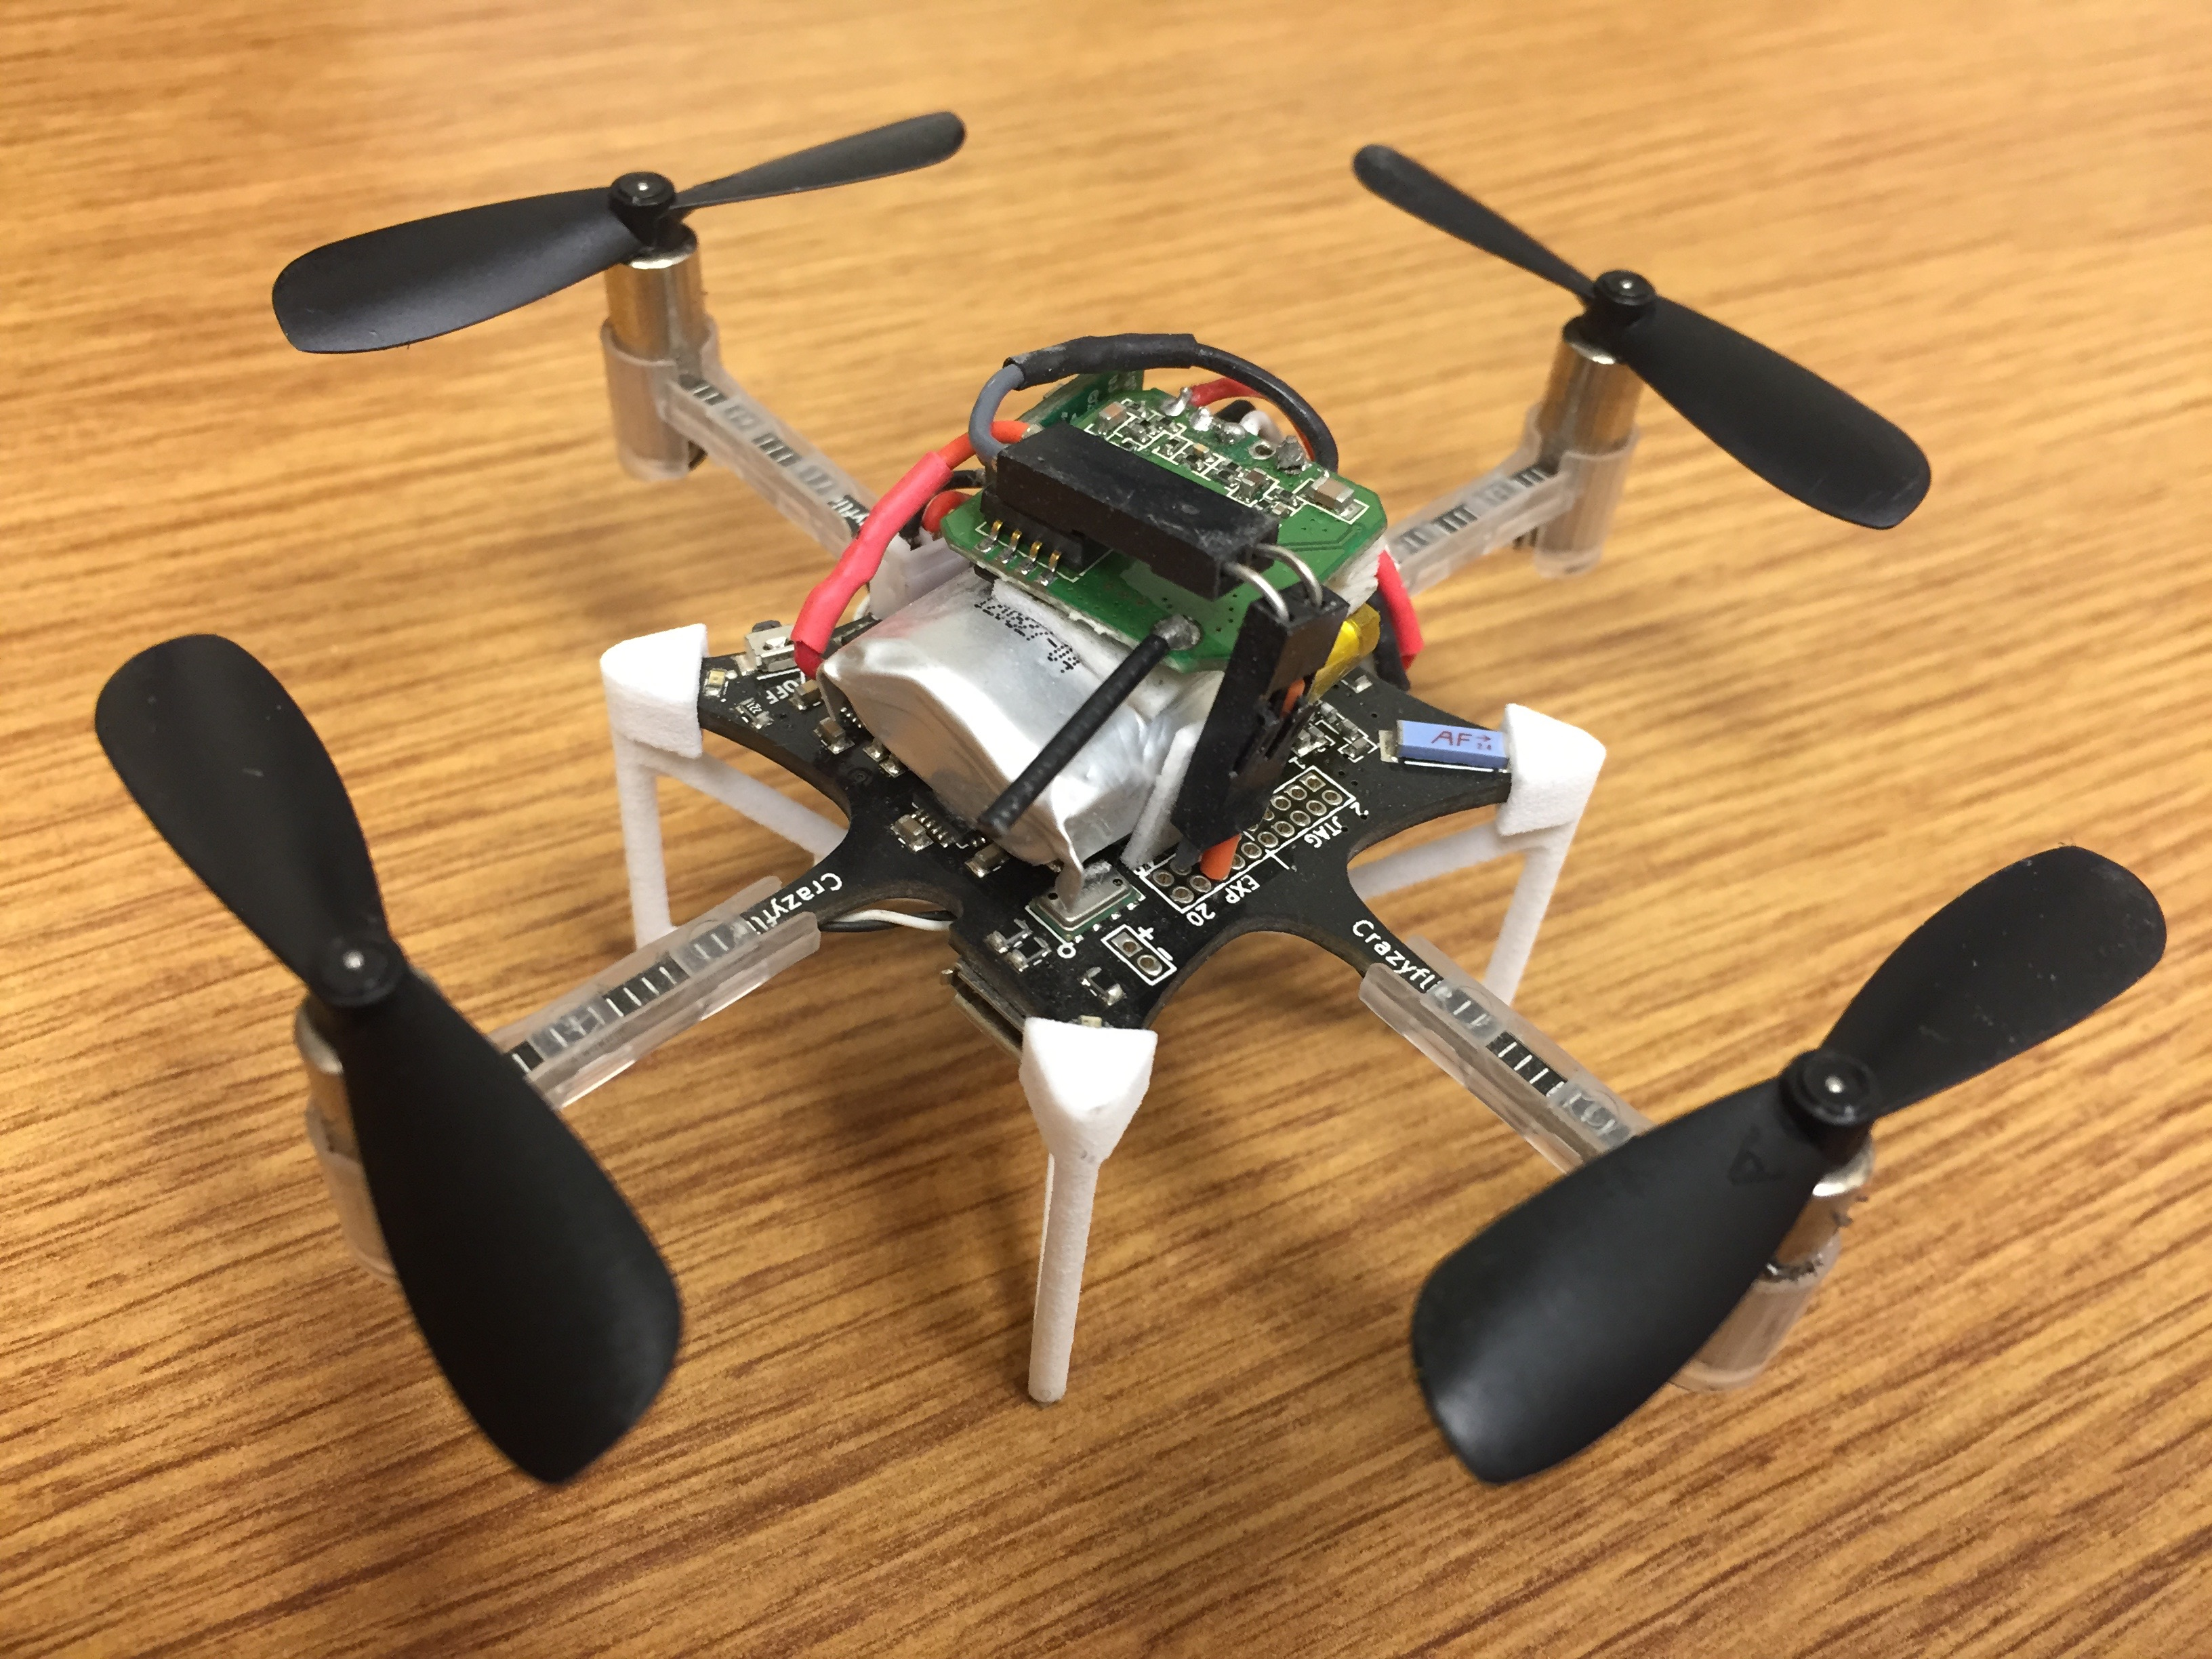
\includegraphics[width=0.5\textwidth]{graphics/crazyflie.jpg}
    \caption{A Crazyflie Nano Quadrotor with a Downward Camera}
    \label{fig:crazyflie}
\end{figure}

In order to solve such problems, a micro quadrotor can be used alternatively. With greater load capacity, a micro quadrotor can equip with various light-weighted devices onboard, such as a wide-angle camera and a companion computer. In addition, more various autopilot systems are available for a micro quadrotor than for a nano quadrotor. For these advantages, a micro quadrotor is expected to be a better research platform for various purposes, and therefore, this research aims for developing a new micro quadrotor system.

\section{Objective}

In this research, we aim for the application and evaluation of the nonlinear attitude control, suggested by Bandyopadhyay and Chung, that was originally designed for a spacecraft \cite{Bandyopadhyay16}. %Nonlinear Attitude Control of Spacecraft with a Large Captured Object
Also, we validate the proposed approach of inner-loop nonlinear attitude control and linear outer-loop position control with feedforward cancellation used in \cite{Morgan16}. In order to implement the control system, we developed a new micro quadrotor system. The quadrotor dynamics is modeled and characterized based on experimental data. Performance of the quadrotor with the nonlinear attitude control is evaluated by both flight experiments and simulations and compared with conventional PID attitude control. In addition, we suggest a computationally-efficient algorithm to estimate the position of the quadrotor by capturing image data of visual markers, and the algorithm is evaluated by experiments, independently from the quadrotor's flight.

\section{Outline}

The thesis is organized as follows. Chapter \ref{ch:system} describes the overview of the quadrotor system. Chapter \ref{ch:system} also describes the hardware specification of each component and the physical properties of the quadrotor. Chapter \ref{ch:control_system} focuses on the dynamic model and the control system. To be more specific, Section \ref{sec:control_system_system_overview} presents the control system overview. Section \ref{sec:coordinate_system} defines the coordinate systems used for the quadrotor system. Section \ref{sec:outer_loop} describes the dynamic model of the quadrotor's translation motion and its position control. Section \ref{sec:inner_loop} presents the dynamics of the quadrotor rotation and the nonlinear attitude control. The proof of the stability of the nonlinear control is also stated in this section. In Section \ref{sec:motor_control}, a model of DC motors is introduced and an open-loop control of the motors is described. Chapter \ref{ch:evaluation} presents the evaluation of the control system that is stated in Chapter \ref{ch:control_system}. In particular, Section \ref{sec:pid} describes an PID attitude control that is compared with the nonlinear control system. Section \ref{sec:simulation} discusses numerical simulation results of the nonlinear and PID attitude control of the quadrotor. In Section \ref{sec:experiment}, the results of flight experiments are presented with various inputs. Chapter \ref{ch:vision_based_control} introduces a computationally-efficient method to estimate the quadrotor position with given image data of visual markers, and discusses performance of the algorithm. Finally, Chapter \ref{ch:conclusion} summarizes the contents of this thesis and suggests future works.

\chapter{System and Hardware Description}
\label{ch:system}
This research aims for the development and validation of a dynamic model based nonlinear attitude control for a quadrotor. In this chapter, the hardware requirements, specifications, and physical properties of the quadrotor system will be explored.

%%%%%%%%%
\section{Hardware Requirements}
An ordinary quadrotor system is equipped with a micro controller that provides stability and control per inputs from a human user using a radio control (RC) transmitter or a preprogrammed autonomous operation. In order to achieve implementation of a dynamic model based nonlinear attitude controller, the quadrotor must meet the following requirements:
\begin{itemize}
\item All the physical parameters used in the nonlinear control system must be characterized.
\item The quadrotor must provide full access of its control and measurement, and they must be reprogrammable by a user. 
\item The quadrotor must use wireless communication methods to access sensor values and setpoints.
\item The quadrotor must be able to execute an algorithm for autonomous operation either offboard or onboard.
\end{itemize}
To satisfy these requirements, an offboard control system is used for the validation of the nonlinear attitude control and the evaluation of its performance. The system consists of an autopilot controller, actuators, and wireless communication interface including radio telemetry and a backup RC controller with human pilot. PX4, an open-source autopilot system, is installed in the autopilot, and it runs with a nonlinear controller. Also, all the physical parameters used in the control system are measured and characterized. They are described in Section 2.2, 2.3 and 3.5.

In addition to the development of the control system for the quadrotor, in order to implement a vision-based position estimator, the quadrotor must have sufficient computing power to process visual data. The autopilot's microcontroller does not have sufficient power to process visual data and execute the autonomous operation algorithm by itself. Therefore, an external processor is necessary. The processor can be either onboard the quadrotor or offboard. If the processor is onboard the quadrotor, then the quadrotor is now a more complex system, with higher power requirements and additional weight from the processor. The processing power would also be restricted due to size, weight, and power limitations. If the processor is offboard in a ground control station, then there would no longer be restrictions on the size, weight, and power. However, this method increases latency. Since quadrotors are agile systems, low latency computation is preferred, and therefore, an onboard companion computer is added to the quadrotor system in order to implement the vision-based position estimator.
%%%%%%%%%

\section{Hardware Specification}
The dimension and mass of each component are shown at Table \ref{table:components_list}.

\begin{table}[h]
\begin{center}
\begin{tabular*}{0.85\textwidth}{@{\extracolsep{\fill} } | c | r | r | }
  \hline
  	Components	& Dimension [\(10^{-3} \text{m}\)] &	Mass [\text{g}] \\
  \hline
  Brushless DC motor &   \( \diameter 28 \times 30\) & \(62\) \\
  Electric Speed Control & \(48 \times 25 \times 5 \) & \(21\) \\
  LiPo Battery & \(129 \times 39 \times 20 \) & \( 216\) \\
  Autopilot Controller & \( 82 \times 50 \times 16 \) & \( 38\) \\
  Onboard Computer & \( 82 \times 58 \times 22 \) & \(60\) \\
  USB Camera & \(38 \times 38 \times 24 \) & \(15\) \\
  RC Receiver & \( 32 \times 22 \times 12 \) & \(11\) \\
  Radio Telemetry & \( 160 \times 24 \times 12 \) & \(24\)\\
  \hline
\end{tabular*}
  \caption{Dimension and Mass of Each Component}
  \label{table:components_list}
\end{center}
\end{table}

\subsection{Frame}

In the quadrotor system, a glass fiber X-shaped frame is used, as shown in Figure \ref{fig:geometry}. The length of the quadrotor's arm is 0.225 m and the weight is 0.270 kg. At the end of an arm, a brushless DC motor is installed. To reduce the moment of inertia, an autopilot, a battery, and a power-distribution board are located at the center of the frame. To simplify the dynamic model and decrease sensor errors of the quadrotor's rotational motion, the motors and the autopilot are installed on the same plane of the quadrotor. Electronic Speed Controls (ESCs) are installed on each leg symmetrically. 

\begin{figure}
    \centering
    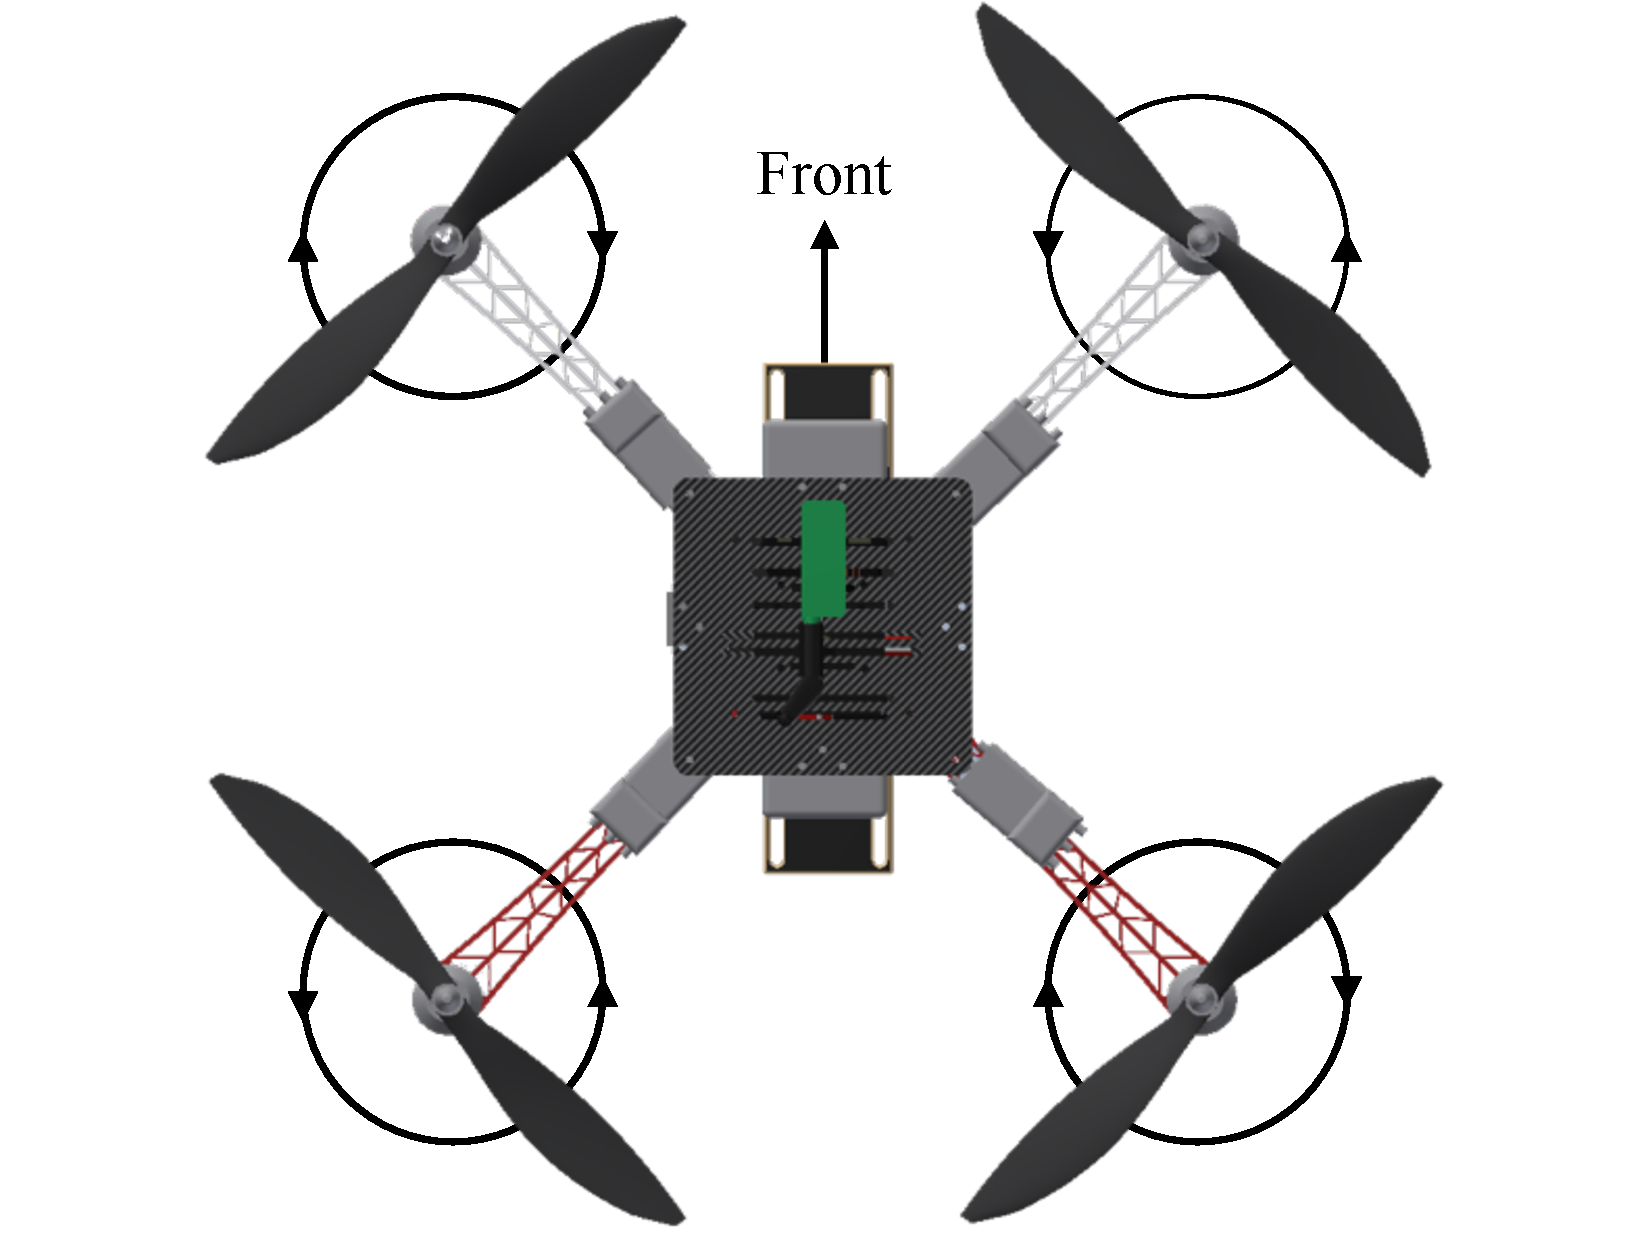
\includegraphics[width=0.5\textwidth]{graphics/geometry.pdf}
    \caption{Illustration of the Quadrotor Frame and the Rotors}
    \label{fig:geometry}
\end{figure}

\subsection{Actuator Motors} 

A quadrotor controls its attitude and thrust by independent inputs of its four motors. AC2830-358 850kV Brushless DC motors developed by 3D Robotics are used in this research \cite{motor}. The maximum power of the motors is 187 W. Since we use brushless DC motors, the quadrotor requires ESCs to run the motors. ESCs are also developed by 3D Robotics \cite{esc}. Power is provided to each motor by an 11.1V 2700mAh 3-cell lithium polymer battery. A motor rotates at a frequency corresponding to its voltage, and the average voltage of a motor can be controlled by Pulse Width Modulation (PWM). Details of motor control are stated in Section 3.5. Each motor spins a propeller, providing thrust and moment to each motor.

\begin{figure}
    \centering
    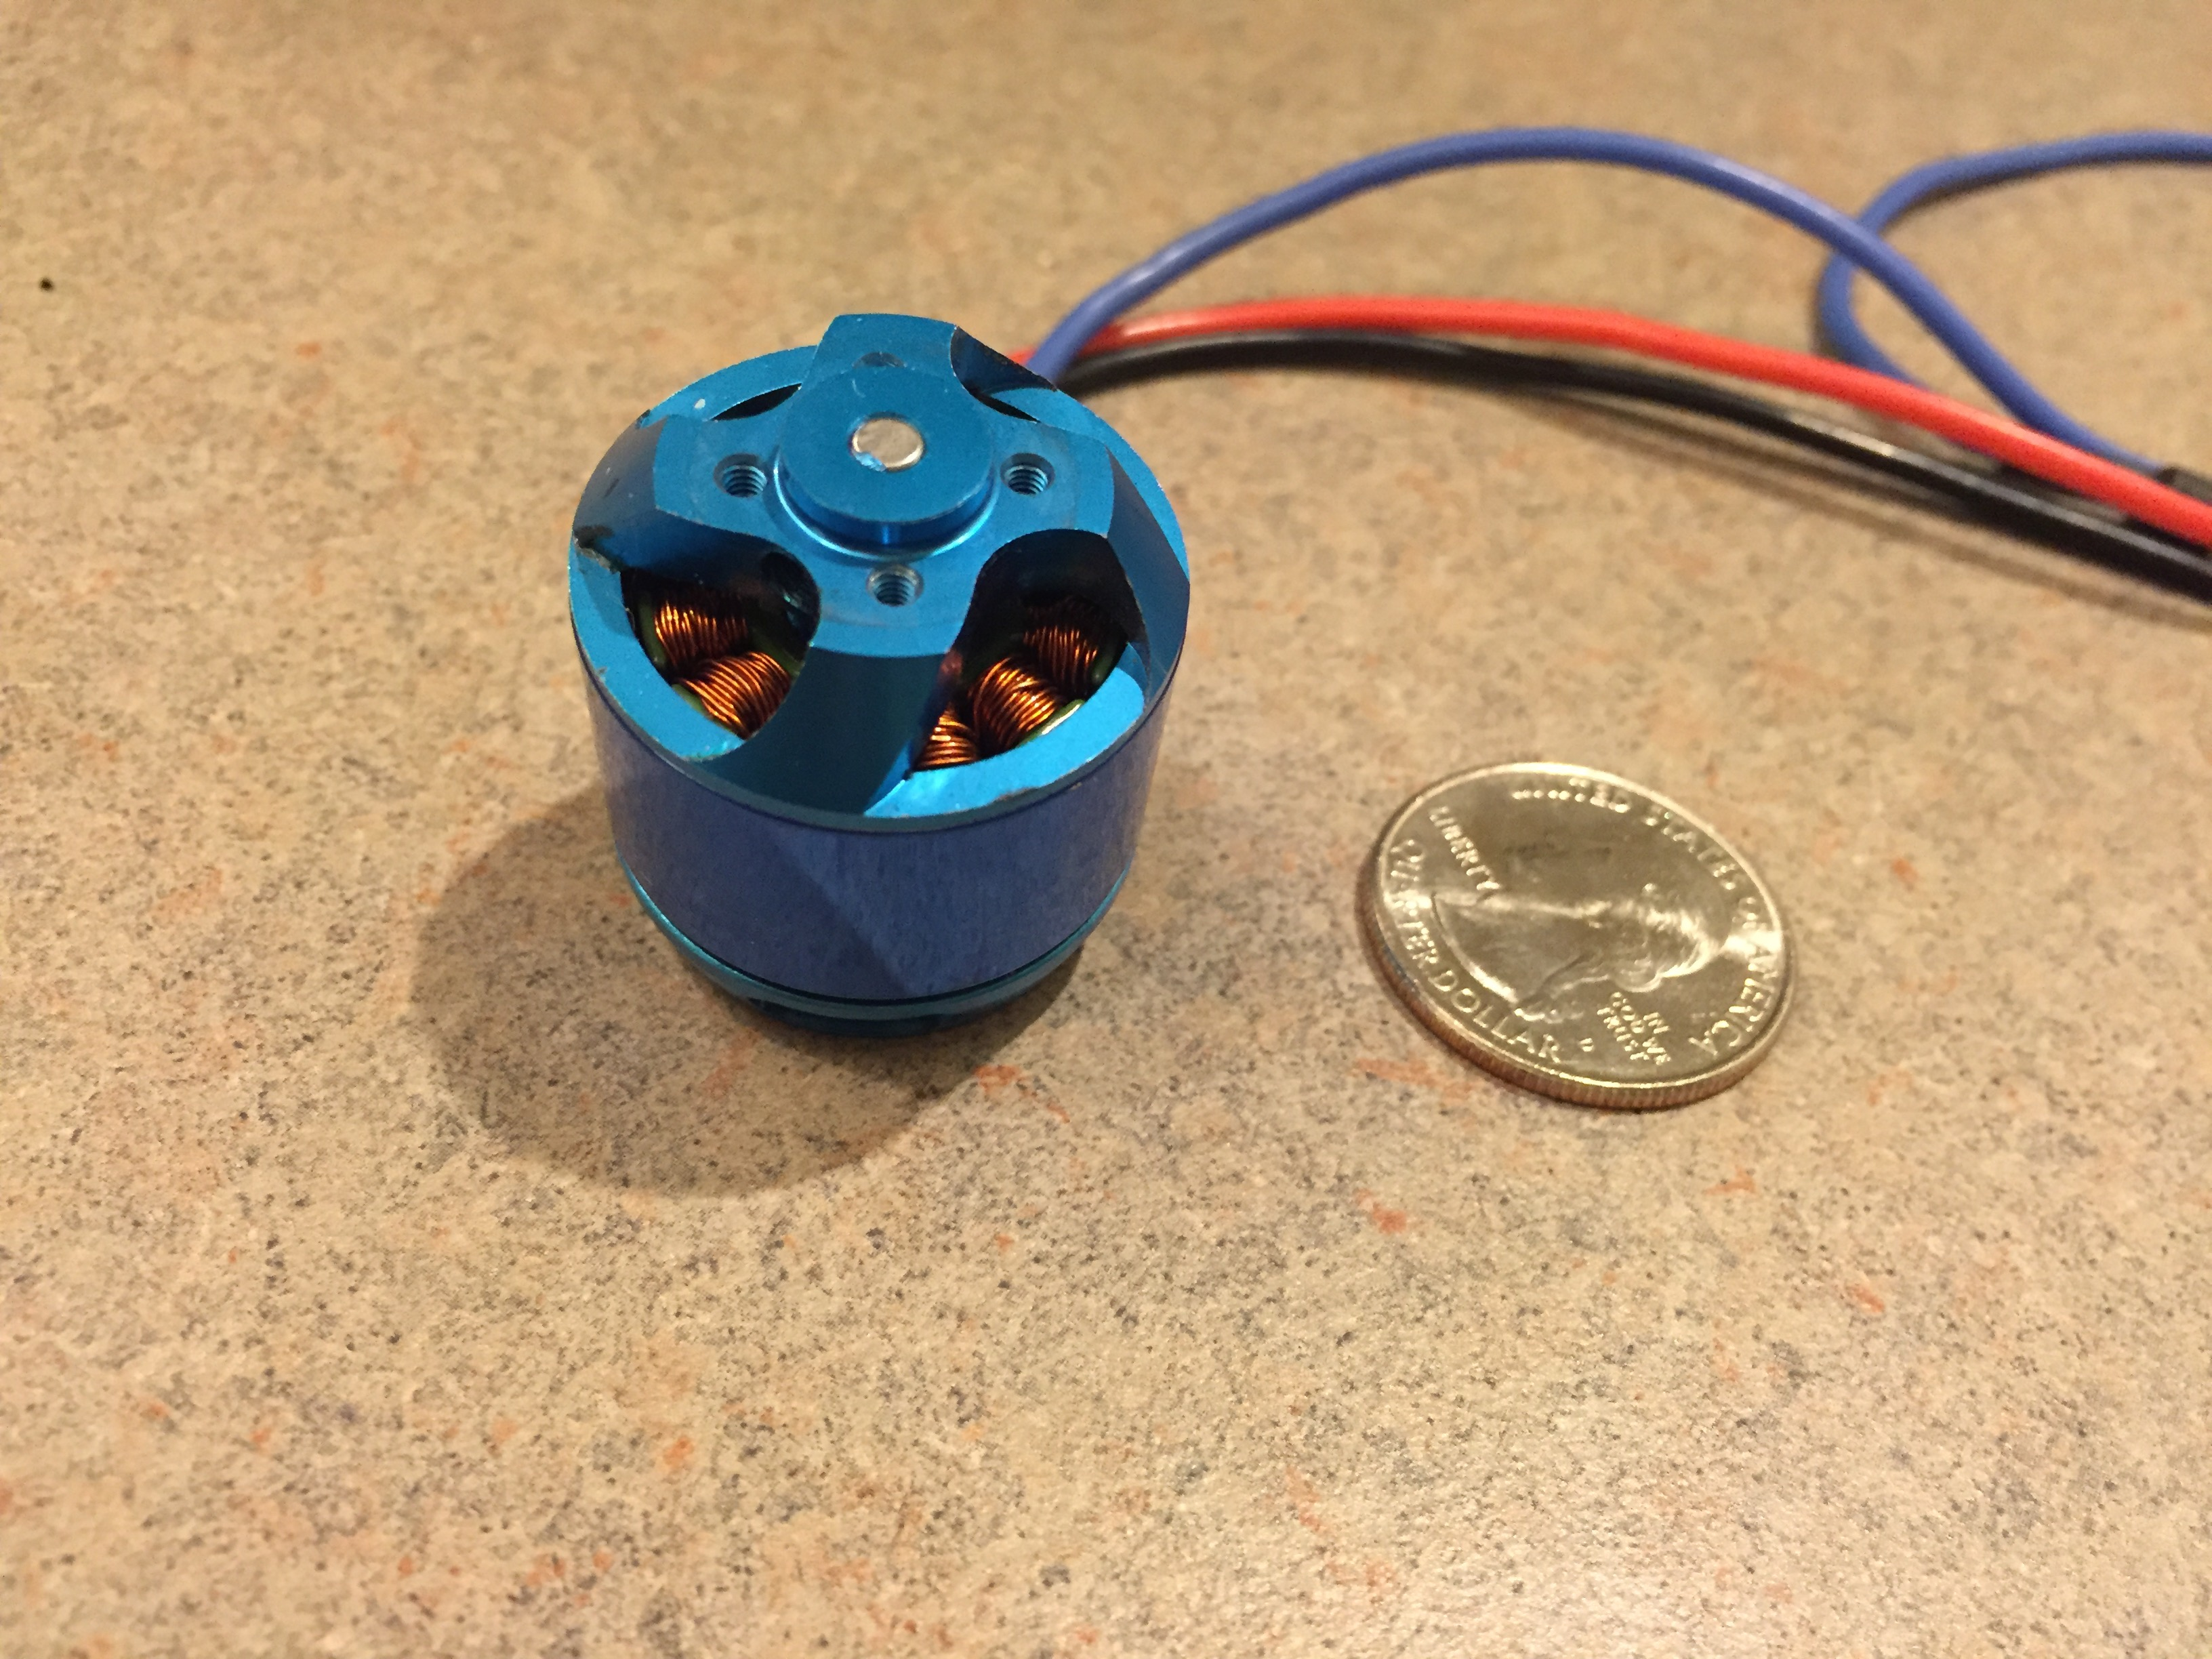
\includegraphics[width=0.5\textwidth]{graphics/motor.jpg}
    \caption{Brushless DC Motor}
    \label{fig:motor}
\end{figure}

\begin{figure}
    \centering
    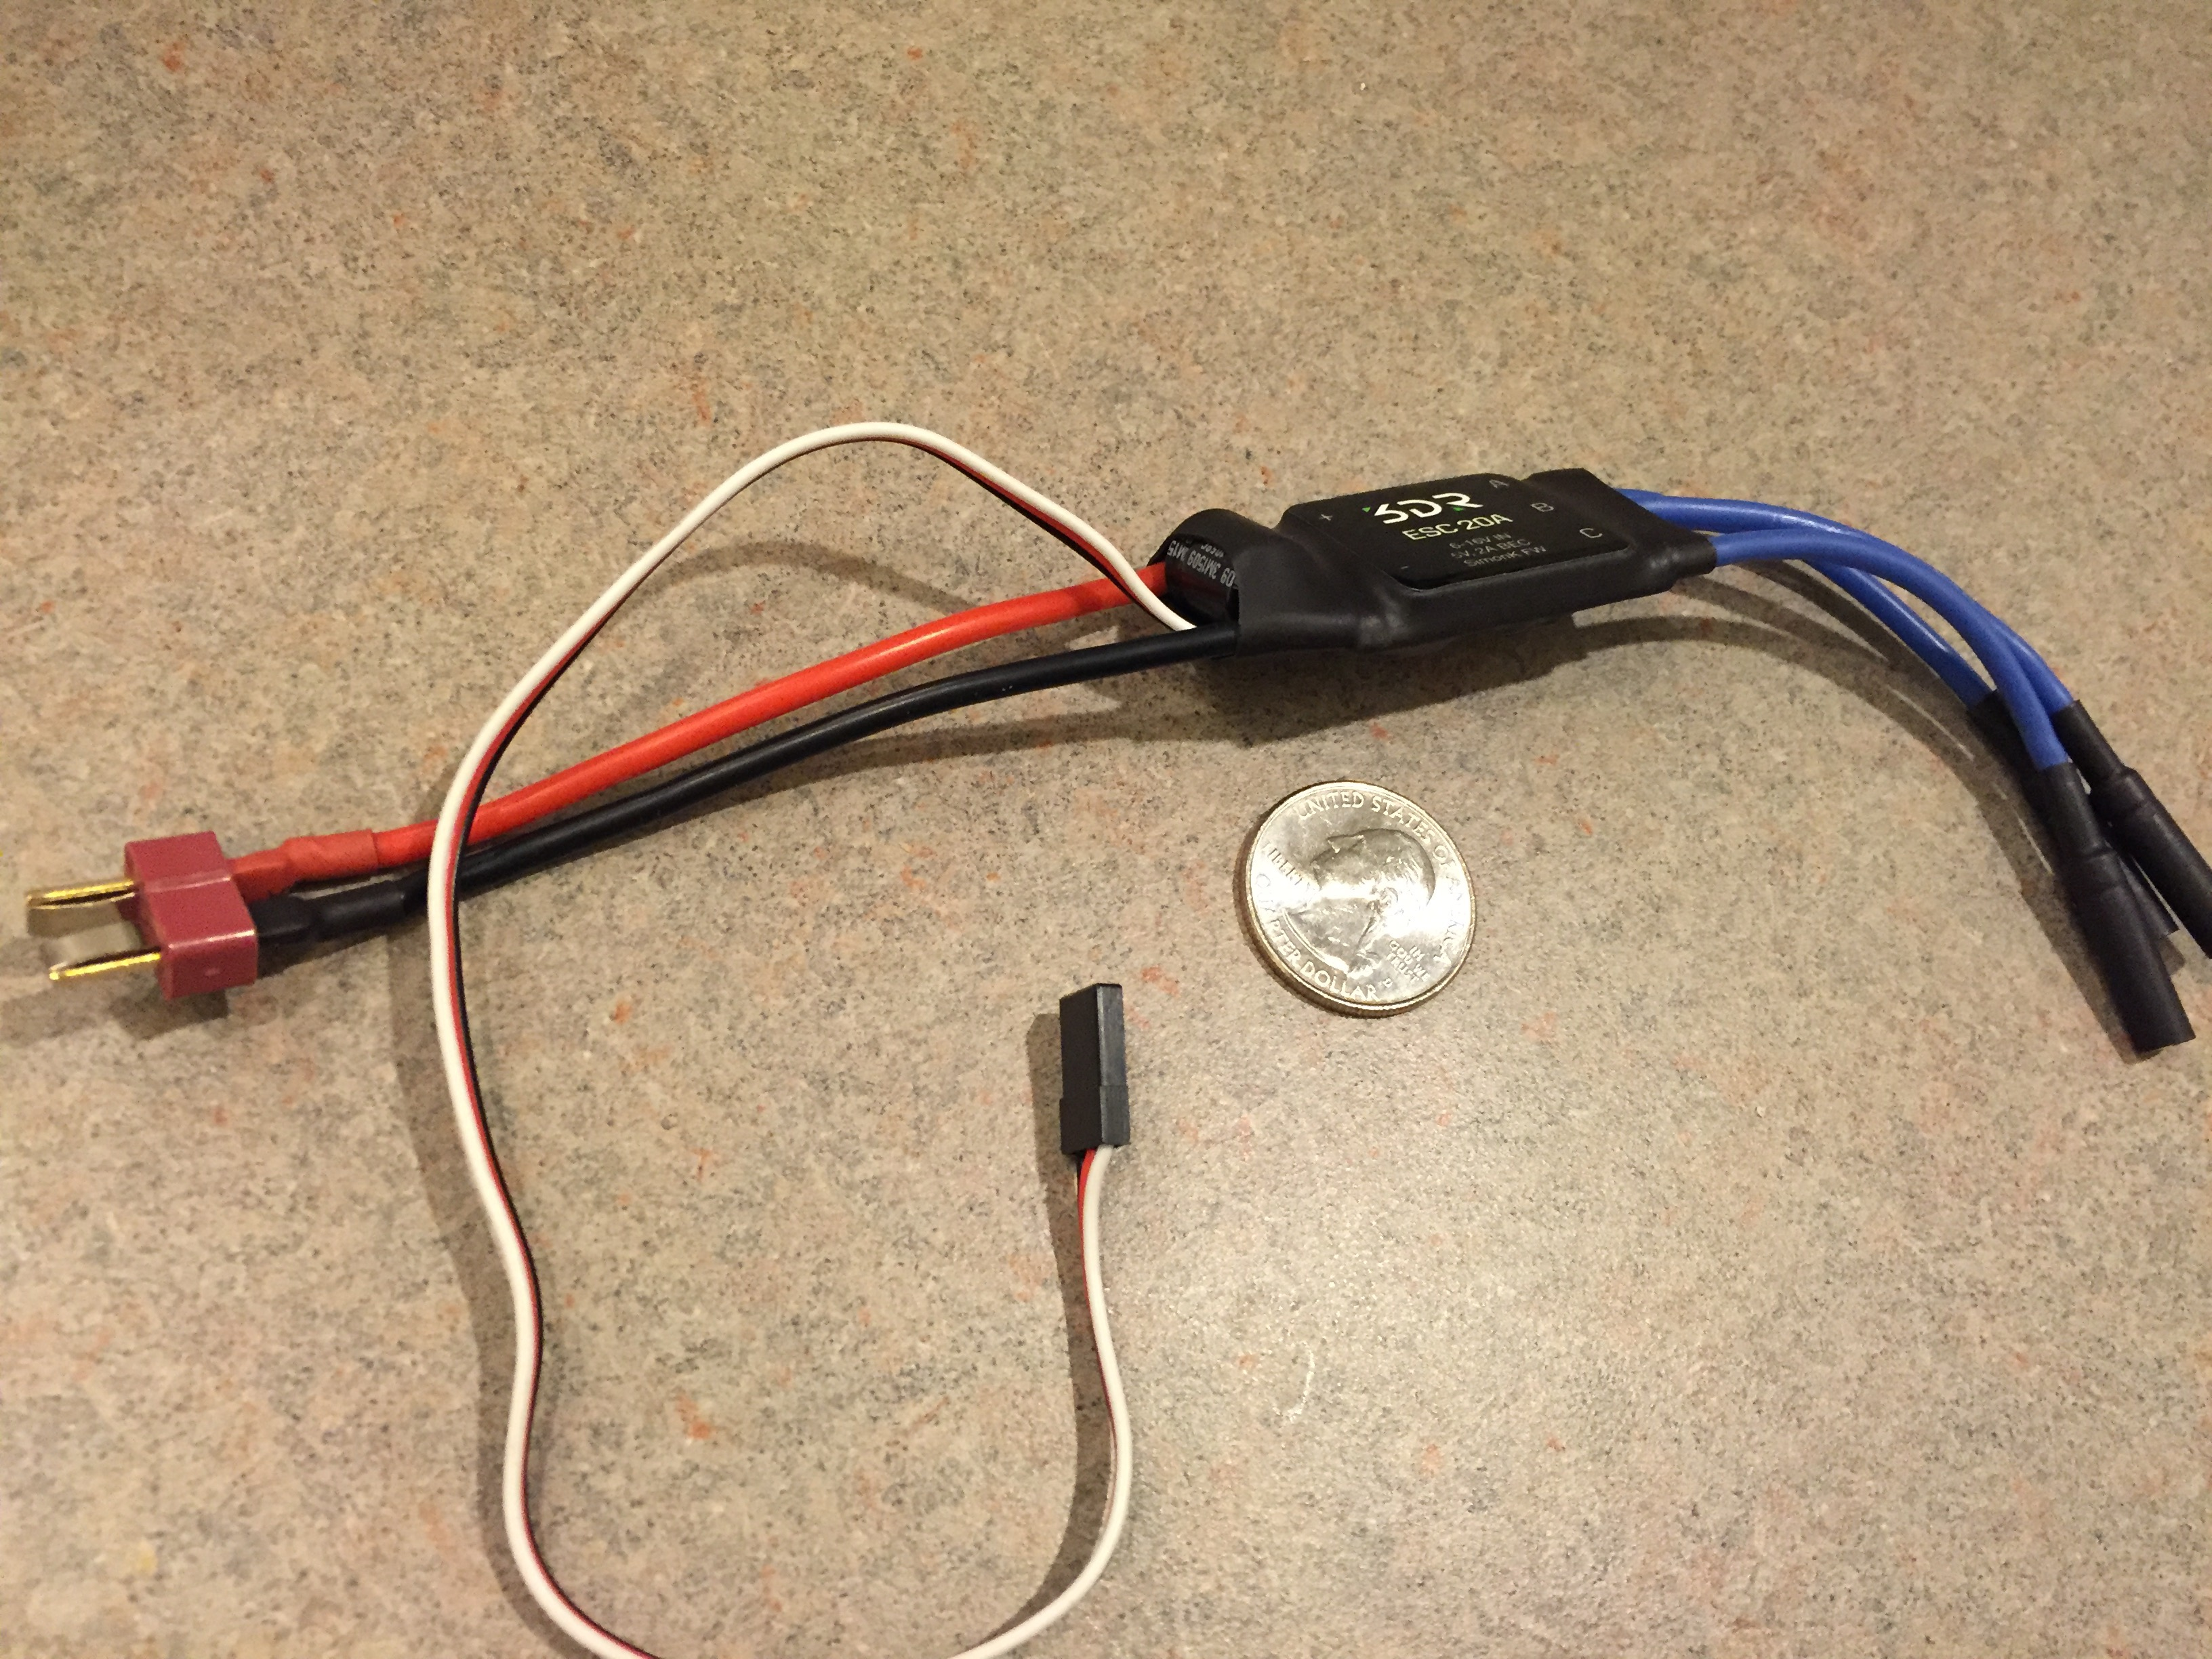
\includegraphics[width=0.5\textwidth]{graphics/esc.jpg}
    \caption{Electric Speed Control (ESC)}
    \label{fig:esc}
  \end{figure}
  
\begin{figure}
    \centering
    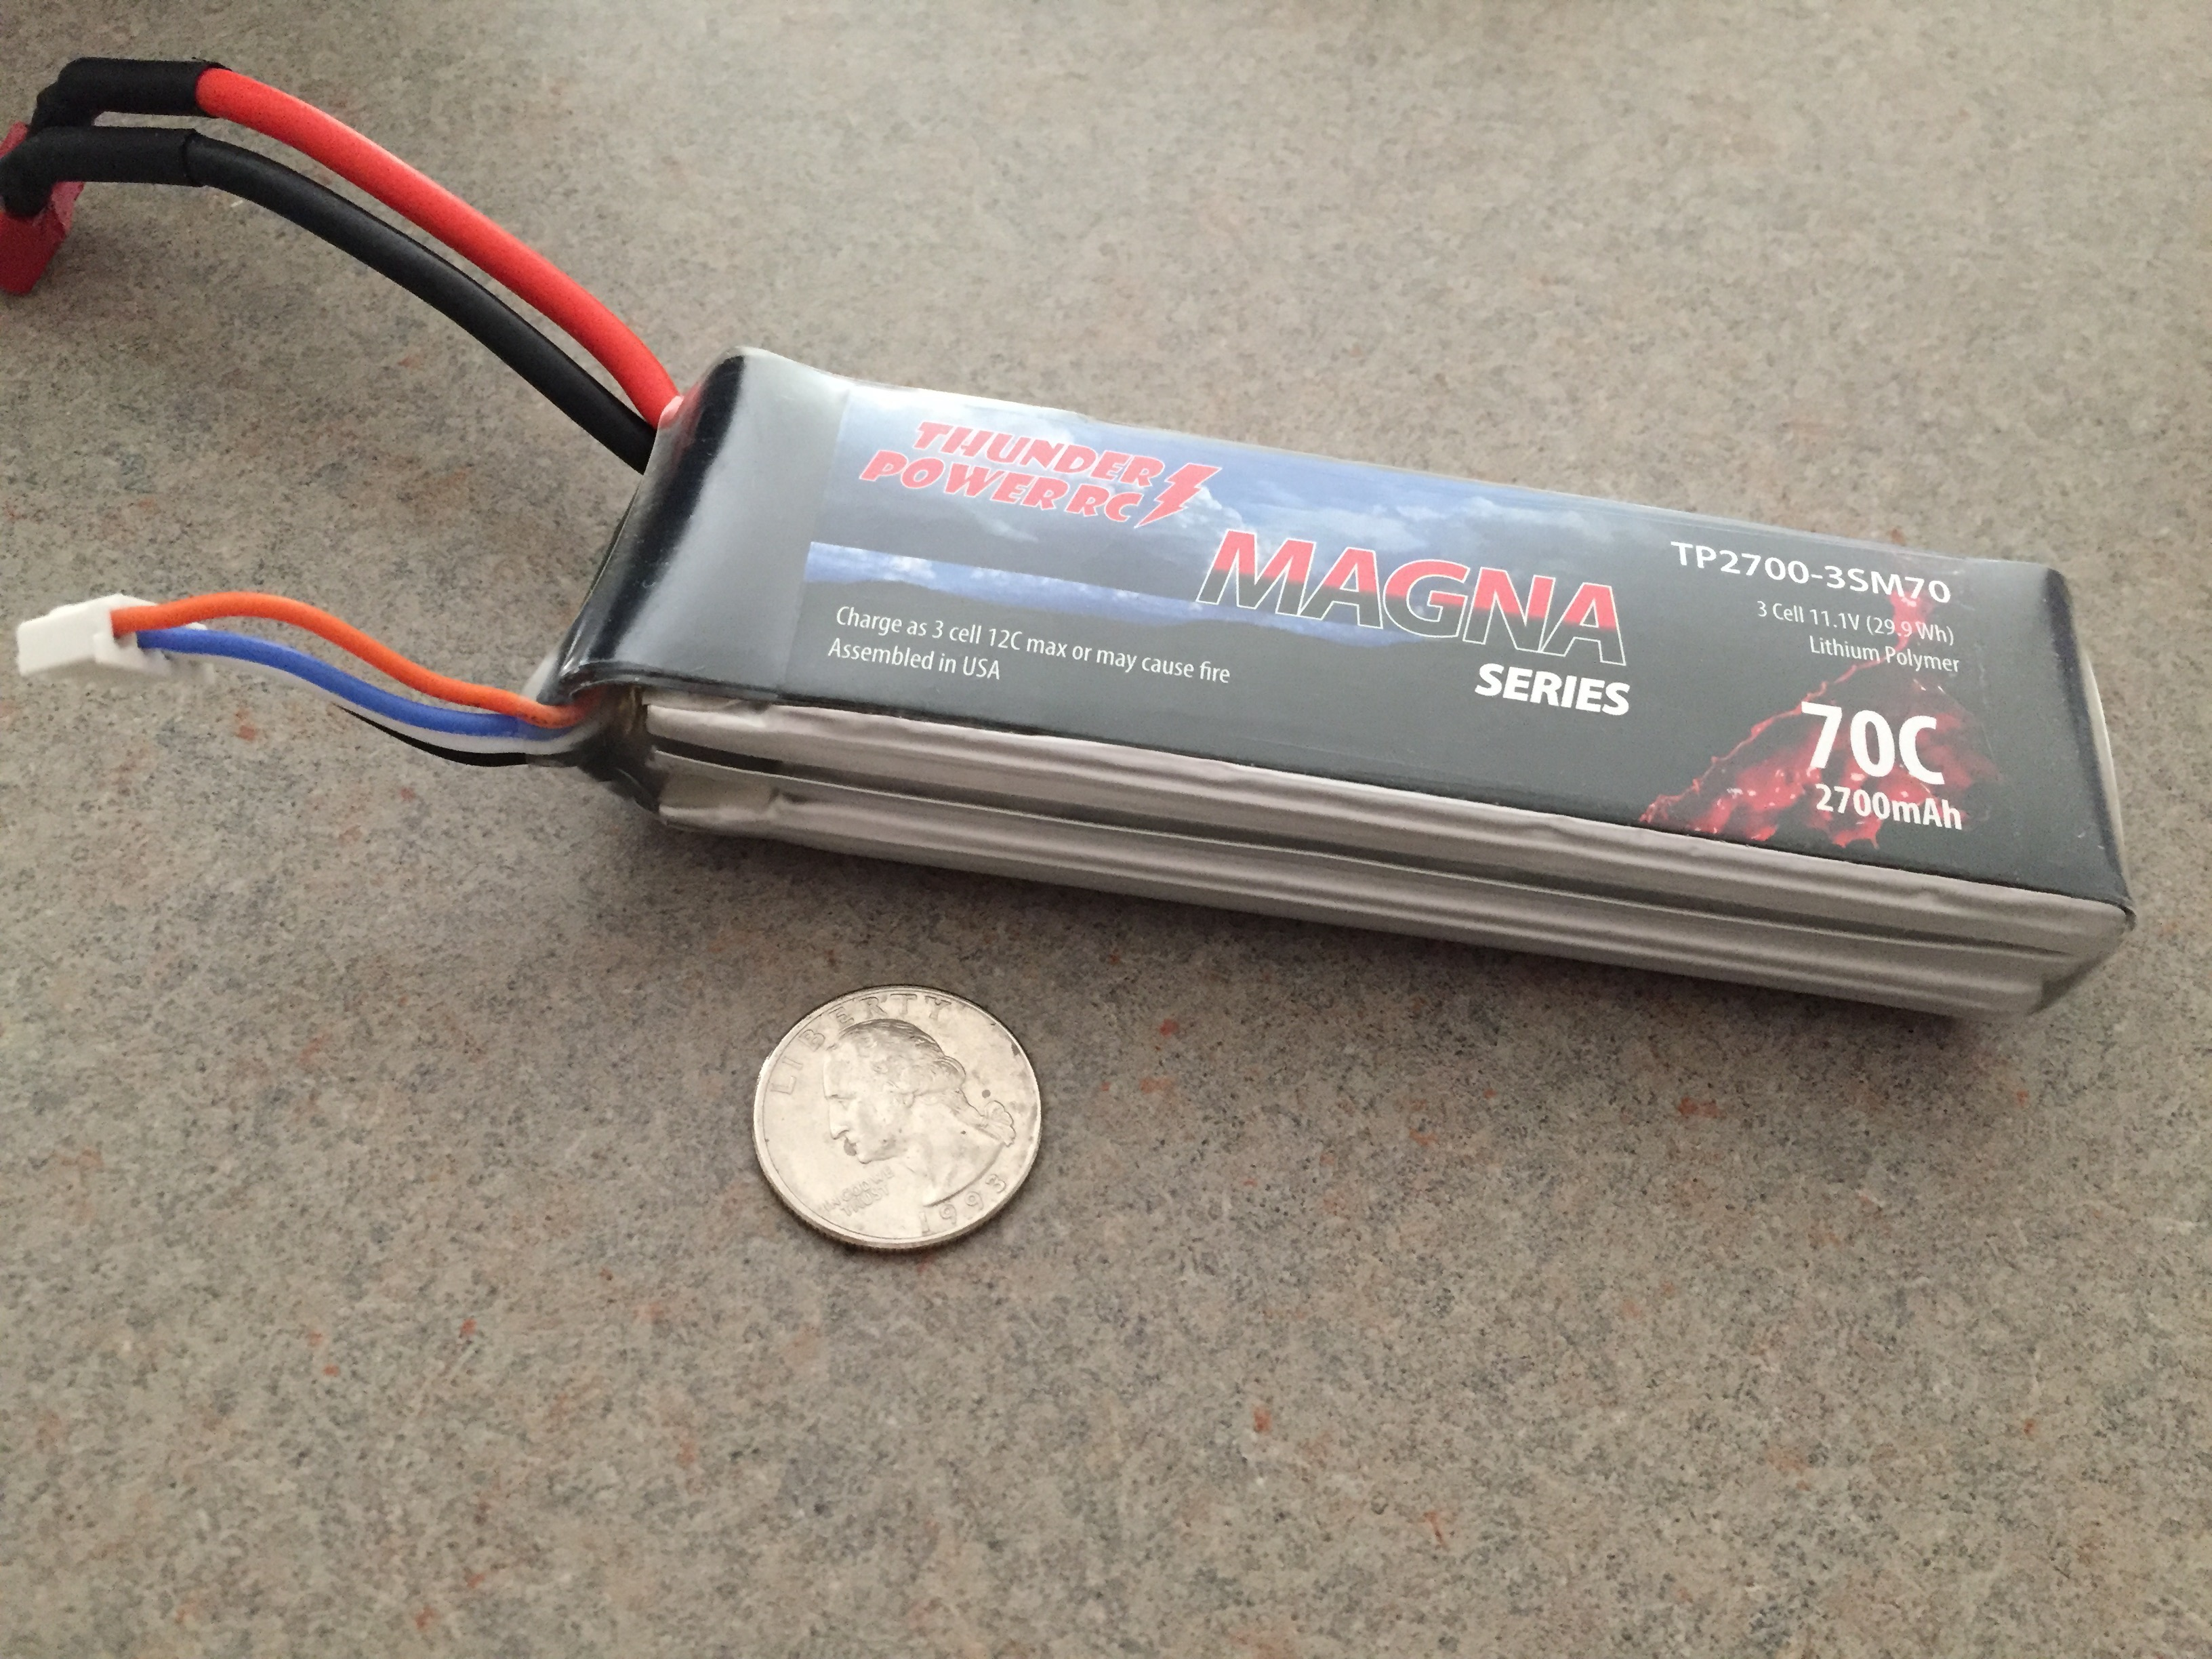
\includegraphics[width=0.5\textwidth]{graphics/battery.jpg}
    \caption{11.1V 2700mAh LiPo Battery}
    \label{fig:battery}
 \end{figure}
 
\subsection{Propeller}

In the quadrotor, two pairs of propellers, APC \(10 \times 4.7\) Slow Flyer (SF) and Slow Flyer Pusher (SFP) propellers, developed by APC Propellers Company, are used \cite{apc}. Both SF and SFP propellers have same geometries as shown at table \ref{table:propeller} but are mirror symmetric to each other. SF propellers are designed to rotate clockwise and SFP propellers are designed to rotate counter-clockwise. As shown in Figure \ref{fig:geometry}, the front-right and rear-left rotors rotate counter-clockwise with SF propellers, and the front-left and rear-right rotors rotate clockwise with SFP propellers. The weight of each propeller is measured as 0.012 kg.

\begin{table}[h]
\begin{center}
\begin{tabular*}{0.85\textwidth}{@{\extracolsep{\fill} } | c | r | r | r | r | }
  \hline
  & 						Entire Diameter &	Hub Diameter &	Hub Thickness &	Shaft Diameter \\
  \hline 
  Length [\(10^{-2} \text{m}\)] & 	{25.4} &		1.27  &			0.74  &			0.64  \\
  \hline
\end{tabular*}
  \caption{Geometry of APC \(10 \times 4.7\) Slow Flyer \cite{airfoil}}
  \label{table:propeller}
\end{center}
\end{table}

\begin{figure}
    \centering
    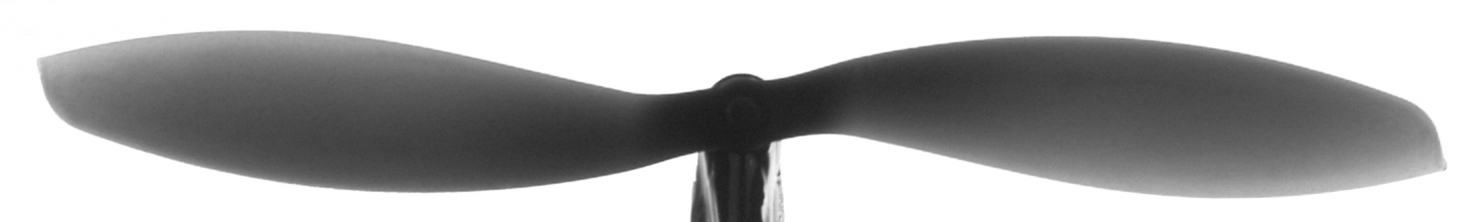
\includegraphics[width=0.8\textwidth]{graphics/apc10x47.jpg}
    \caption{APC  \(10 \times 4.7\) Slow Flyer \cite{airfoil}}
    \label{fig:propeller}
\end{figure}

\subsection{Autopilot}

A quadrotor is typically equipped with a microcontroller autopilot that is controlled by high level commands, such position or attitude setpoints from an RC transmitter. Based on the current state and setpoint commands, the controller computes desired actuation and commands the actuators to respond accordingly. In order to detect the current state, the autopilot requires an accelerometer, gyroscope, and some form of actuator interface in order to function. Since most autopilot systems use a PID controller to control attitude, it is necessary to rewrite the control algorithm. In order to facilitate this, we choose to use the open source PX4 autopilot system \cite{px4}. We used a 3D Robotics Pixhawk microprocessor to run our PX4 code \cite{3dr}. Pixhawk contains all the necessary sensors, computation power, and input/output interfaces. In addition to an accelerometer and a gyroscope, the Pixhawk has a magnetometer and barometer to measure altitude and attitude changes \cite{pixhawk}.

\begin{figure}
    \centering
    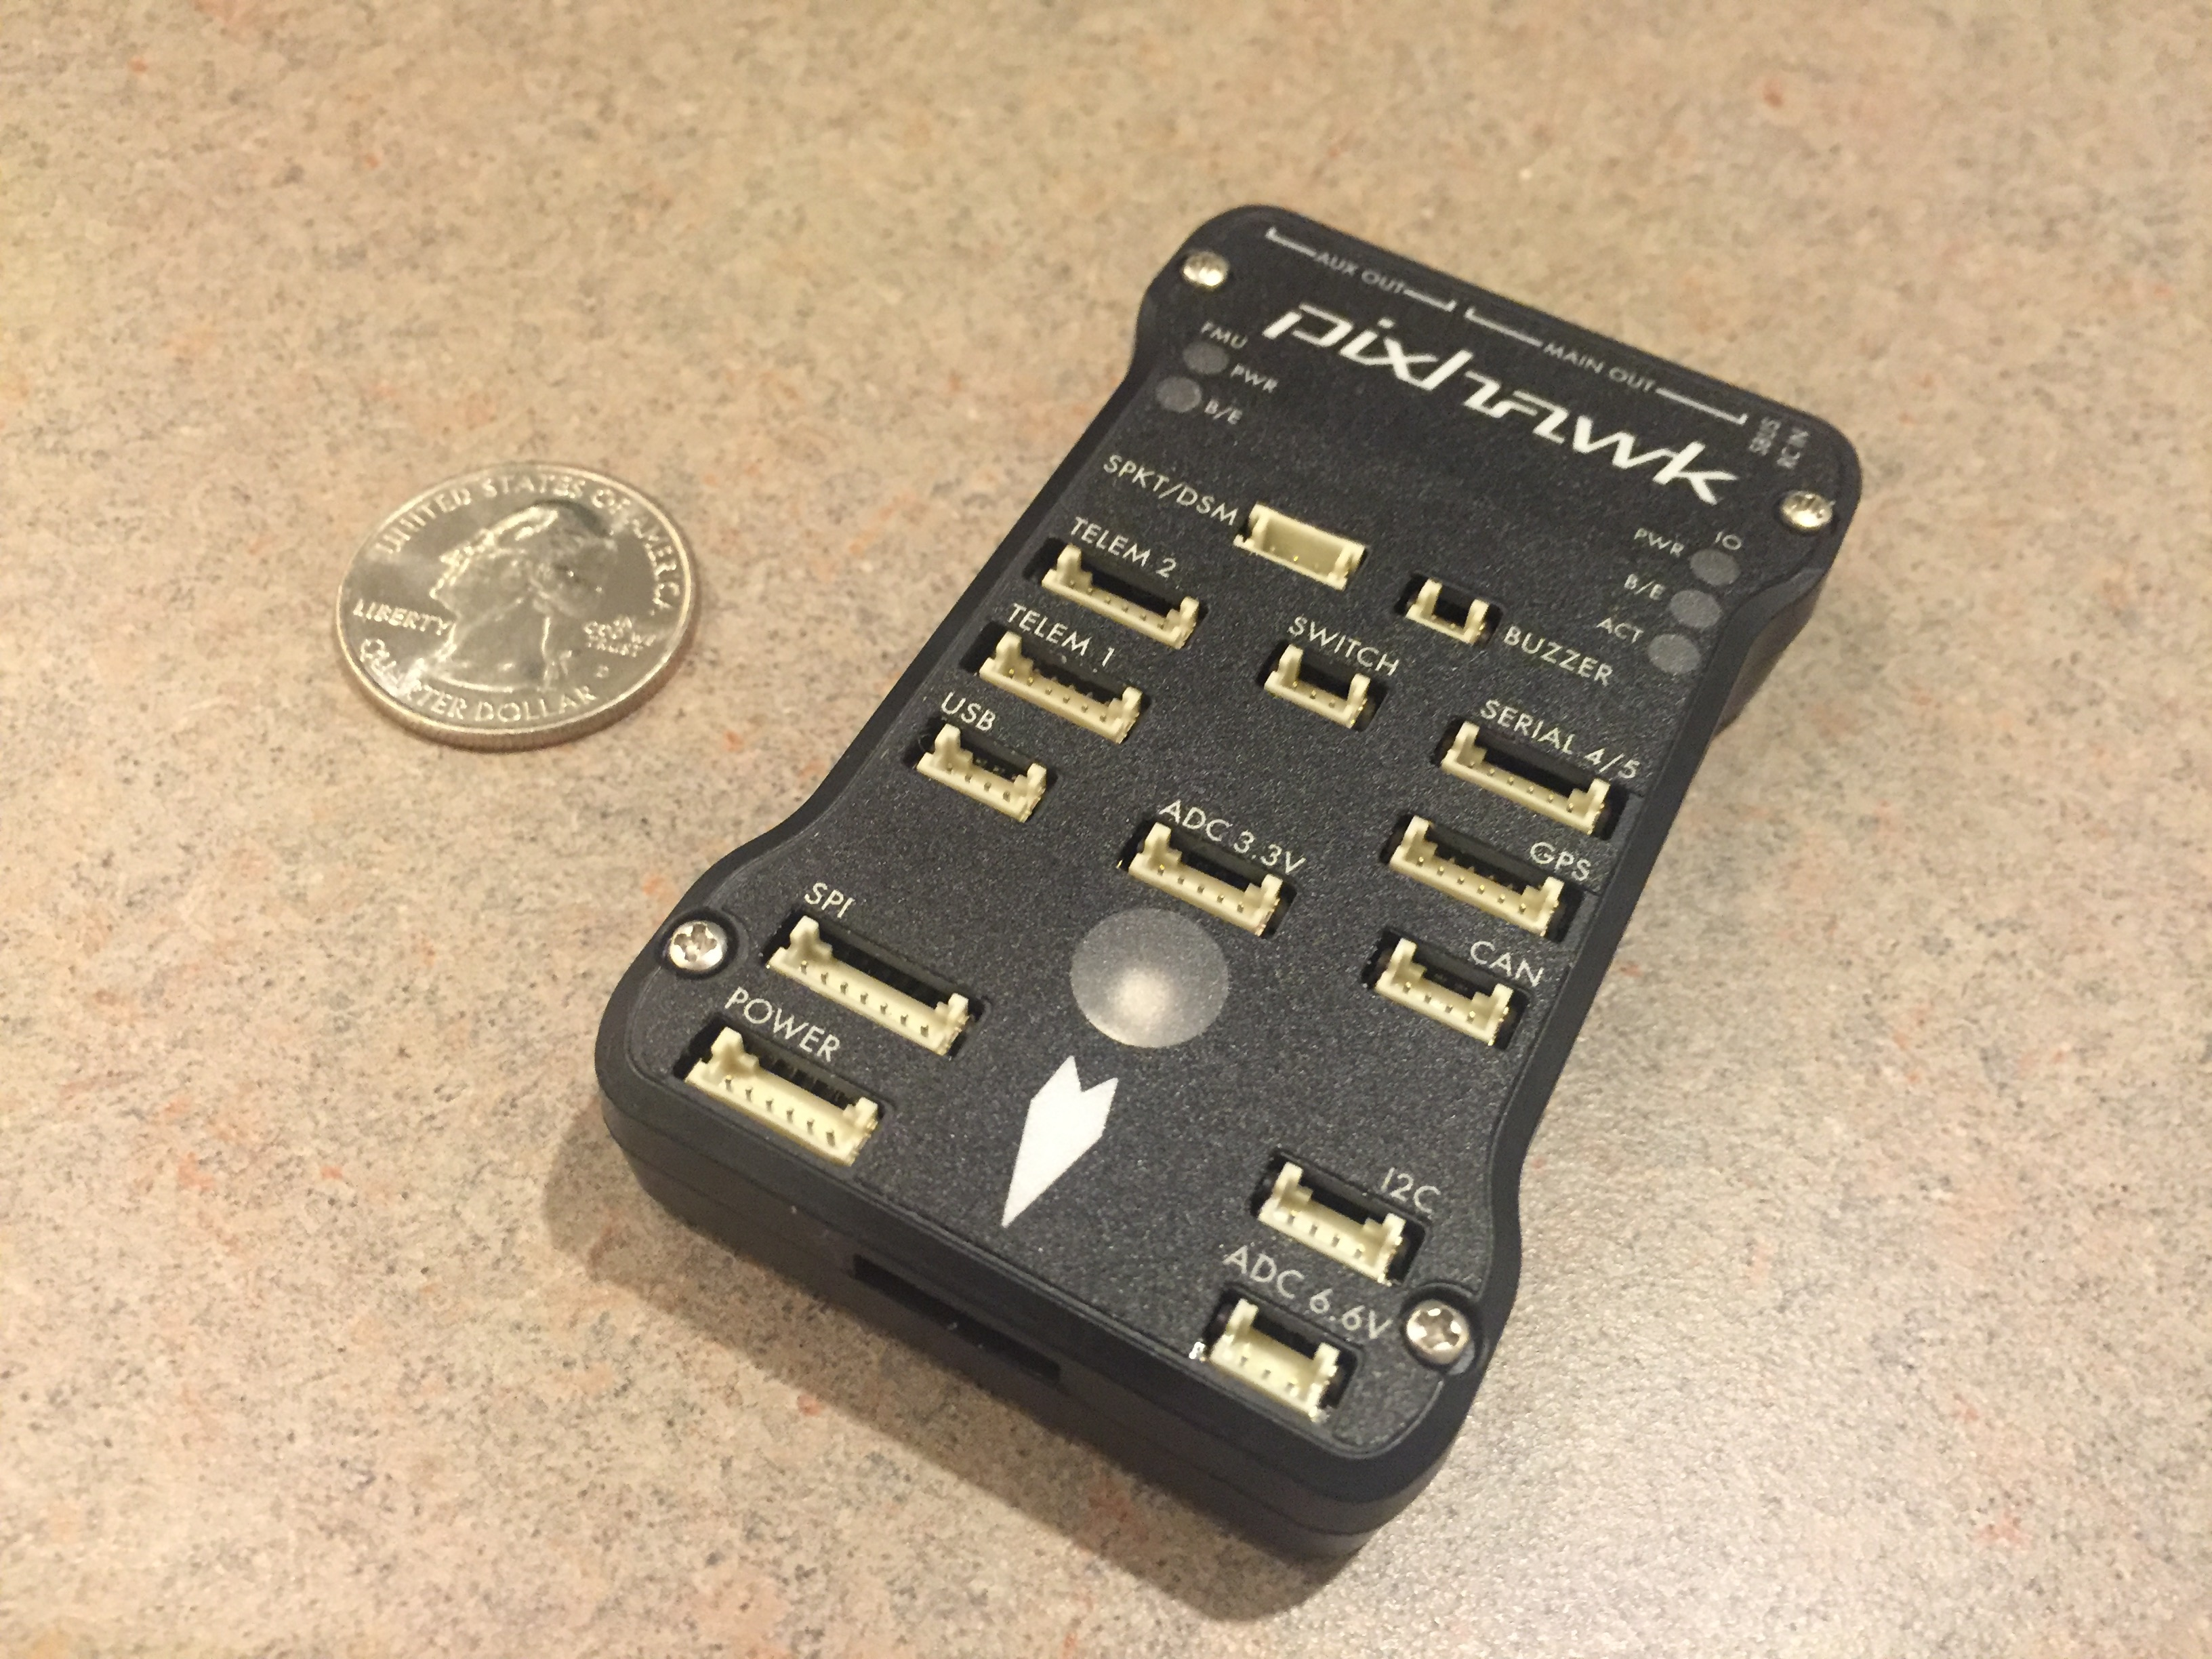
\includegraphics[width=0.5\textwidth]{graphics/pixhawk.jpg}
    \caption{Pixhawk Autopilot}
    \label{fig:pixhawk}
\end{figure}

\subsection{Companion Single-Board Computer}

The companion computer is necessary for estimating the quadrotor position through computer vision. The computer receives image data from a ground facing camera and, using the quadrotor state from the autopilot, computes the position estimation of the quadrotor and sends the estimation data to the autopilot. The quadrotor uses a single Hardkernel Odroid XU4 \cite{hardkernel}. It is a quadcore 1.3 GHz CPU and 2 GB of RAM. The computer runs on a 5 volt 4 amp power supply, which is provided by a voltage converter from the main battery.

\begin{figure}
    \centering
    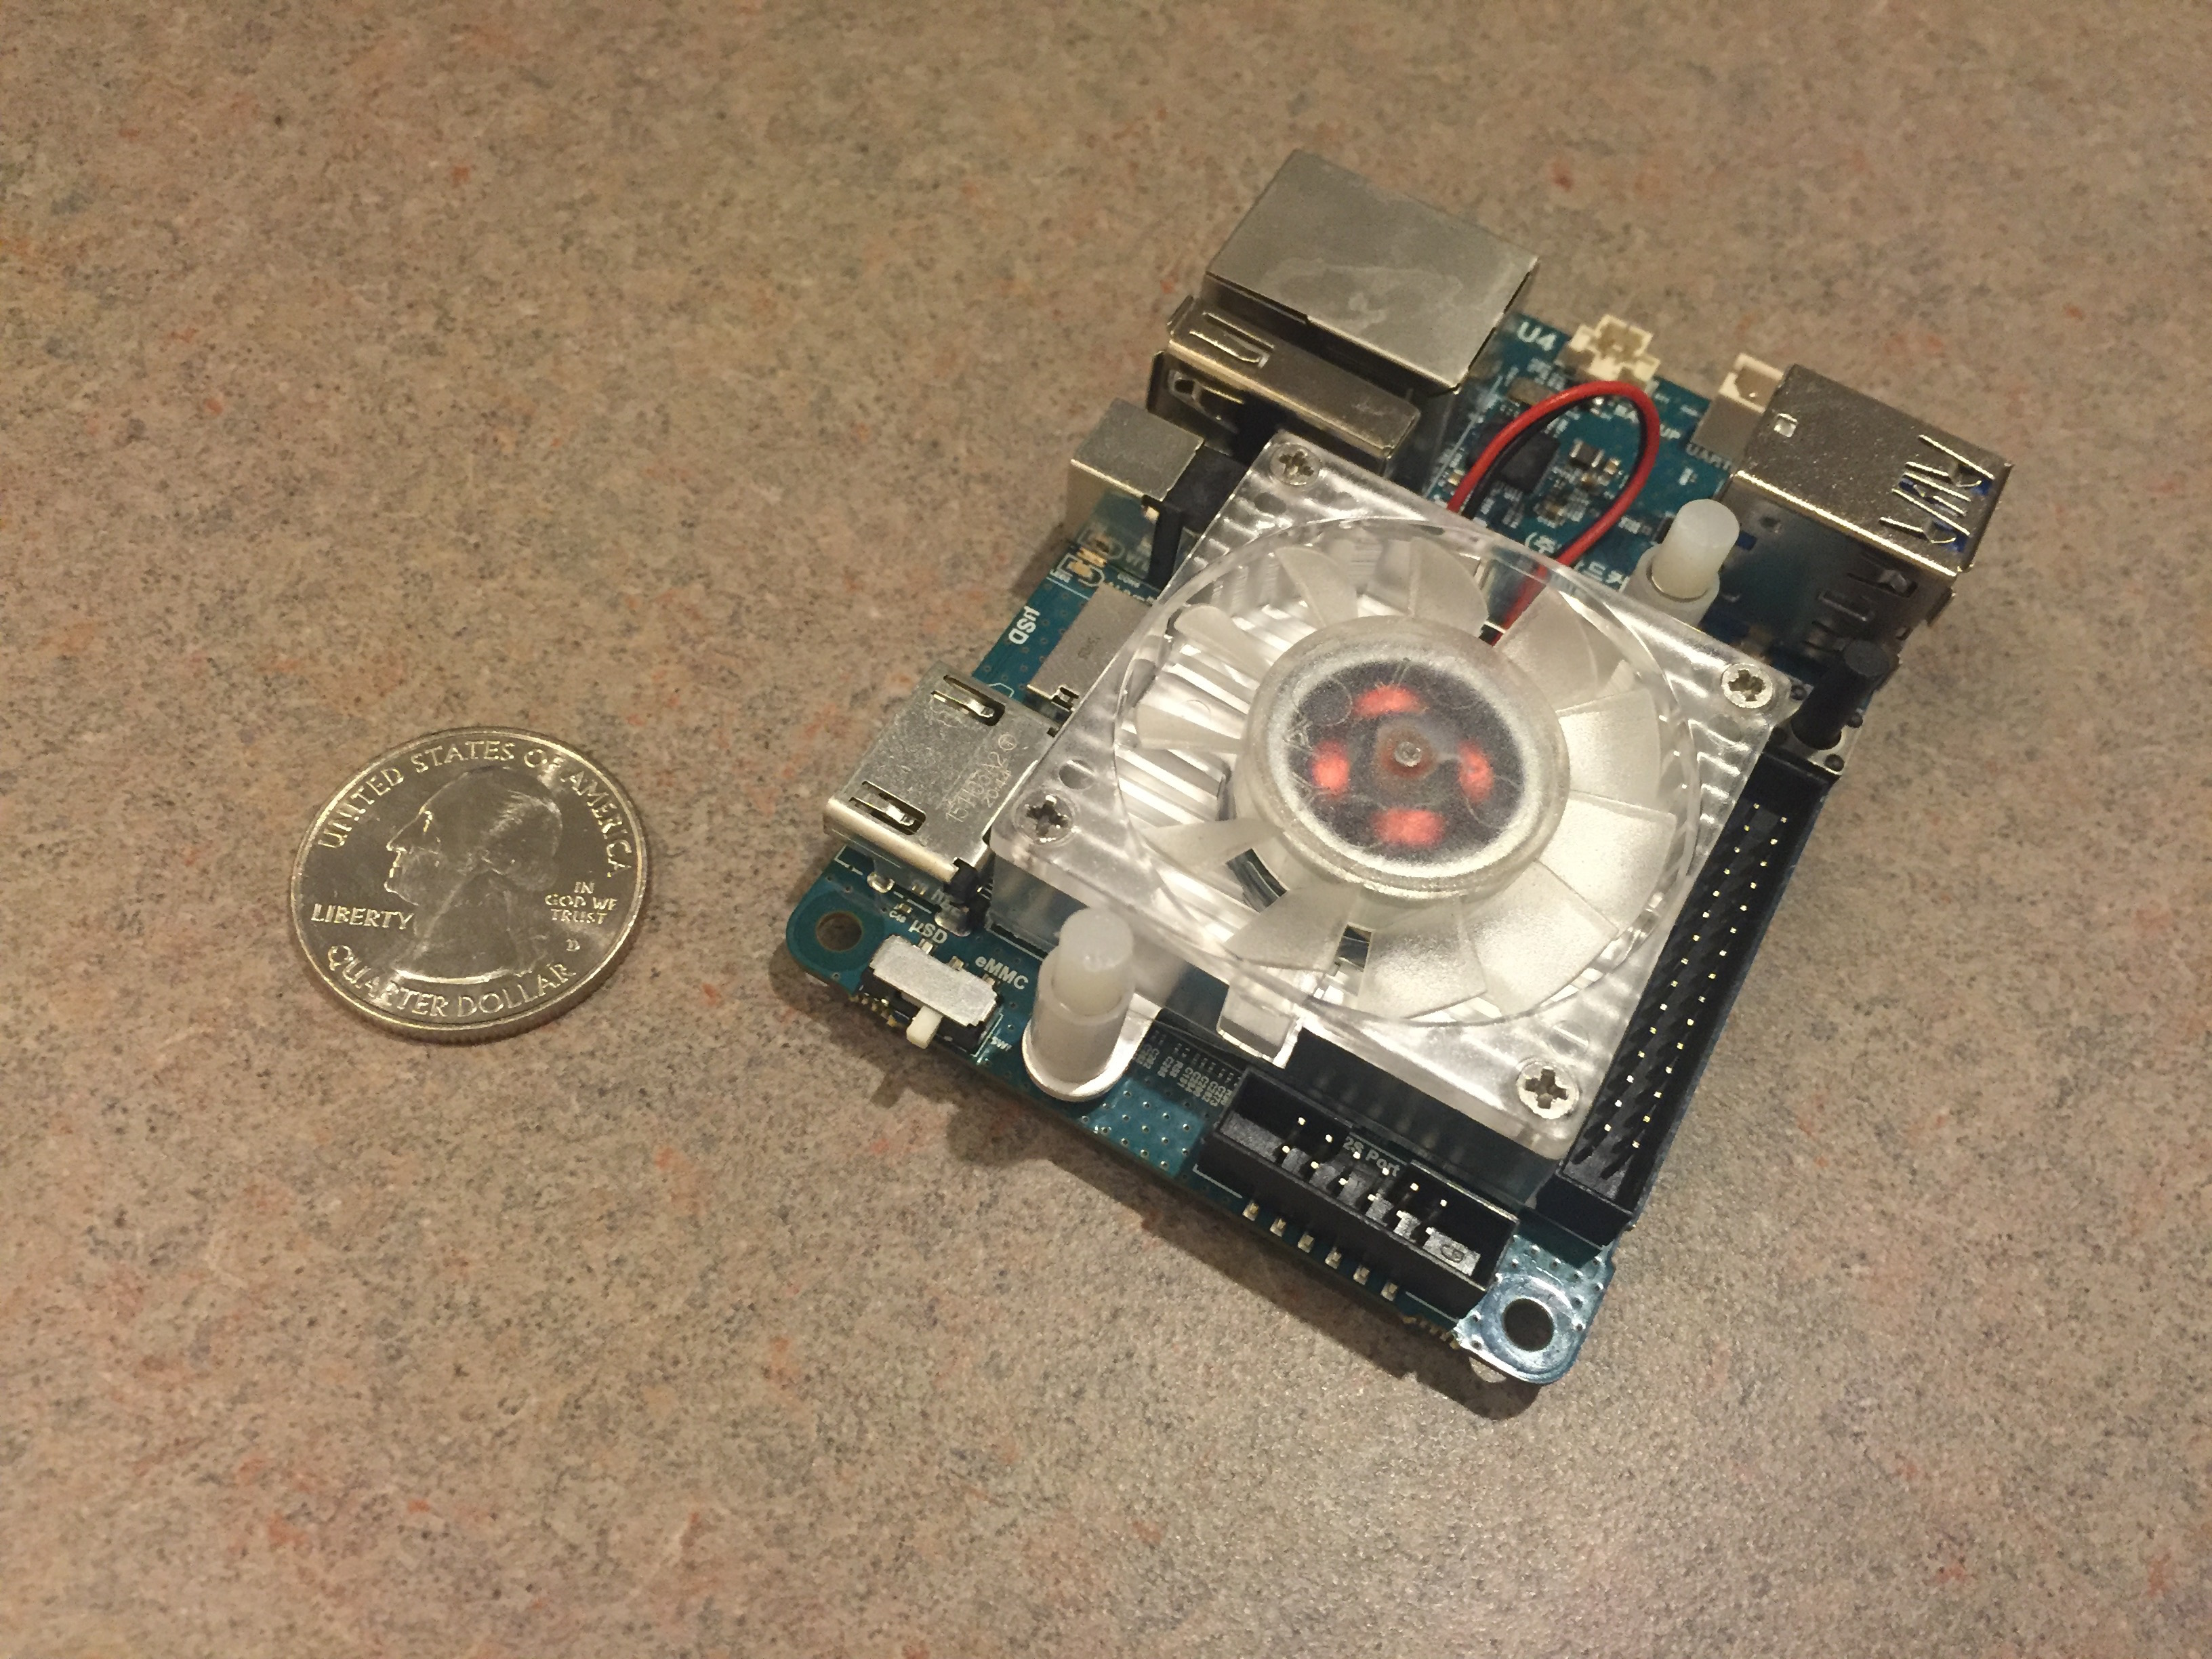
\includegraphics[width=0.5\textwidth]{graphics/odroid.jpg}
    \caption{Odroid XU4 Single-board Computer}
    \label{fig:odroid}
\end{figure}

\subsection{Camera}

The autopilot does not have precise position measurement, so it is necessary to estimate the quadrotor's position precisely using a computer vision system. Four circular markers on the floor are tracked by the quadrotor's camera to provide estimates as to its relative position with respect to the markers. A ground facing camera is used to capture the images of the markers. The USB webcam we use has a focal length of 2.1mm and has about \({120}^{\circ}\) view angle. The camera sends images of \(640 \times 480\) pixels at a rate of 30 frames per second. This sensor is used for vision-based estimation presented in Chapter 5.

\begin{figure}
    \centering
    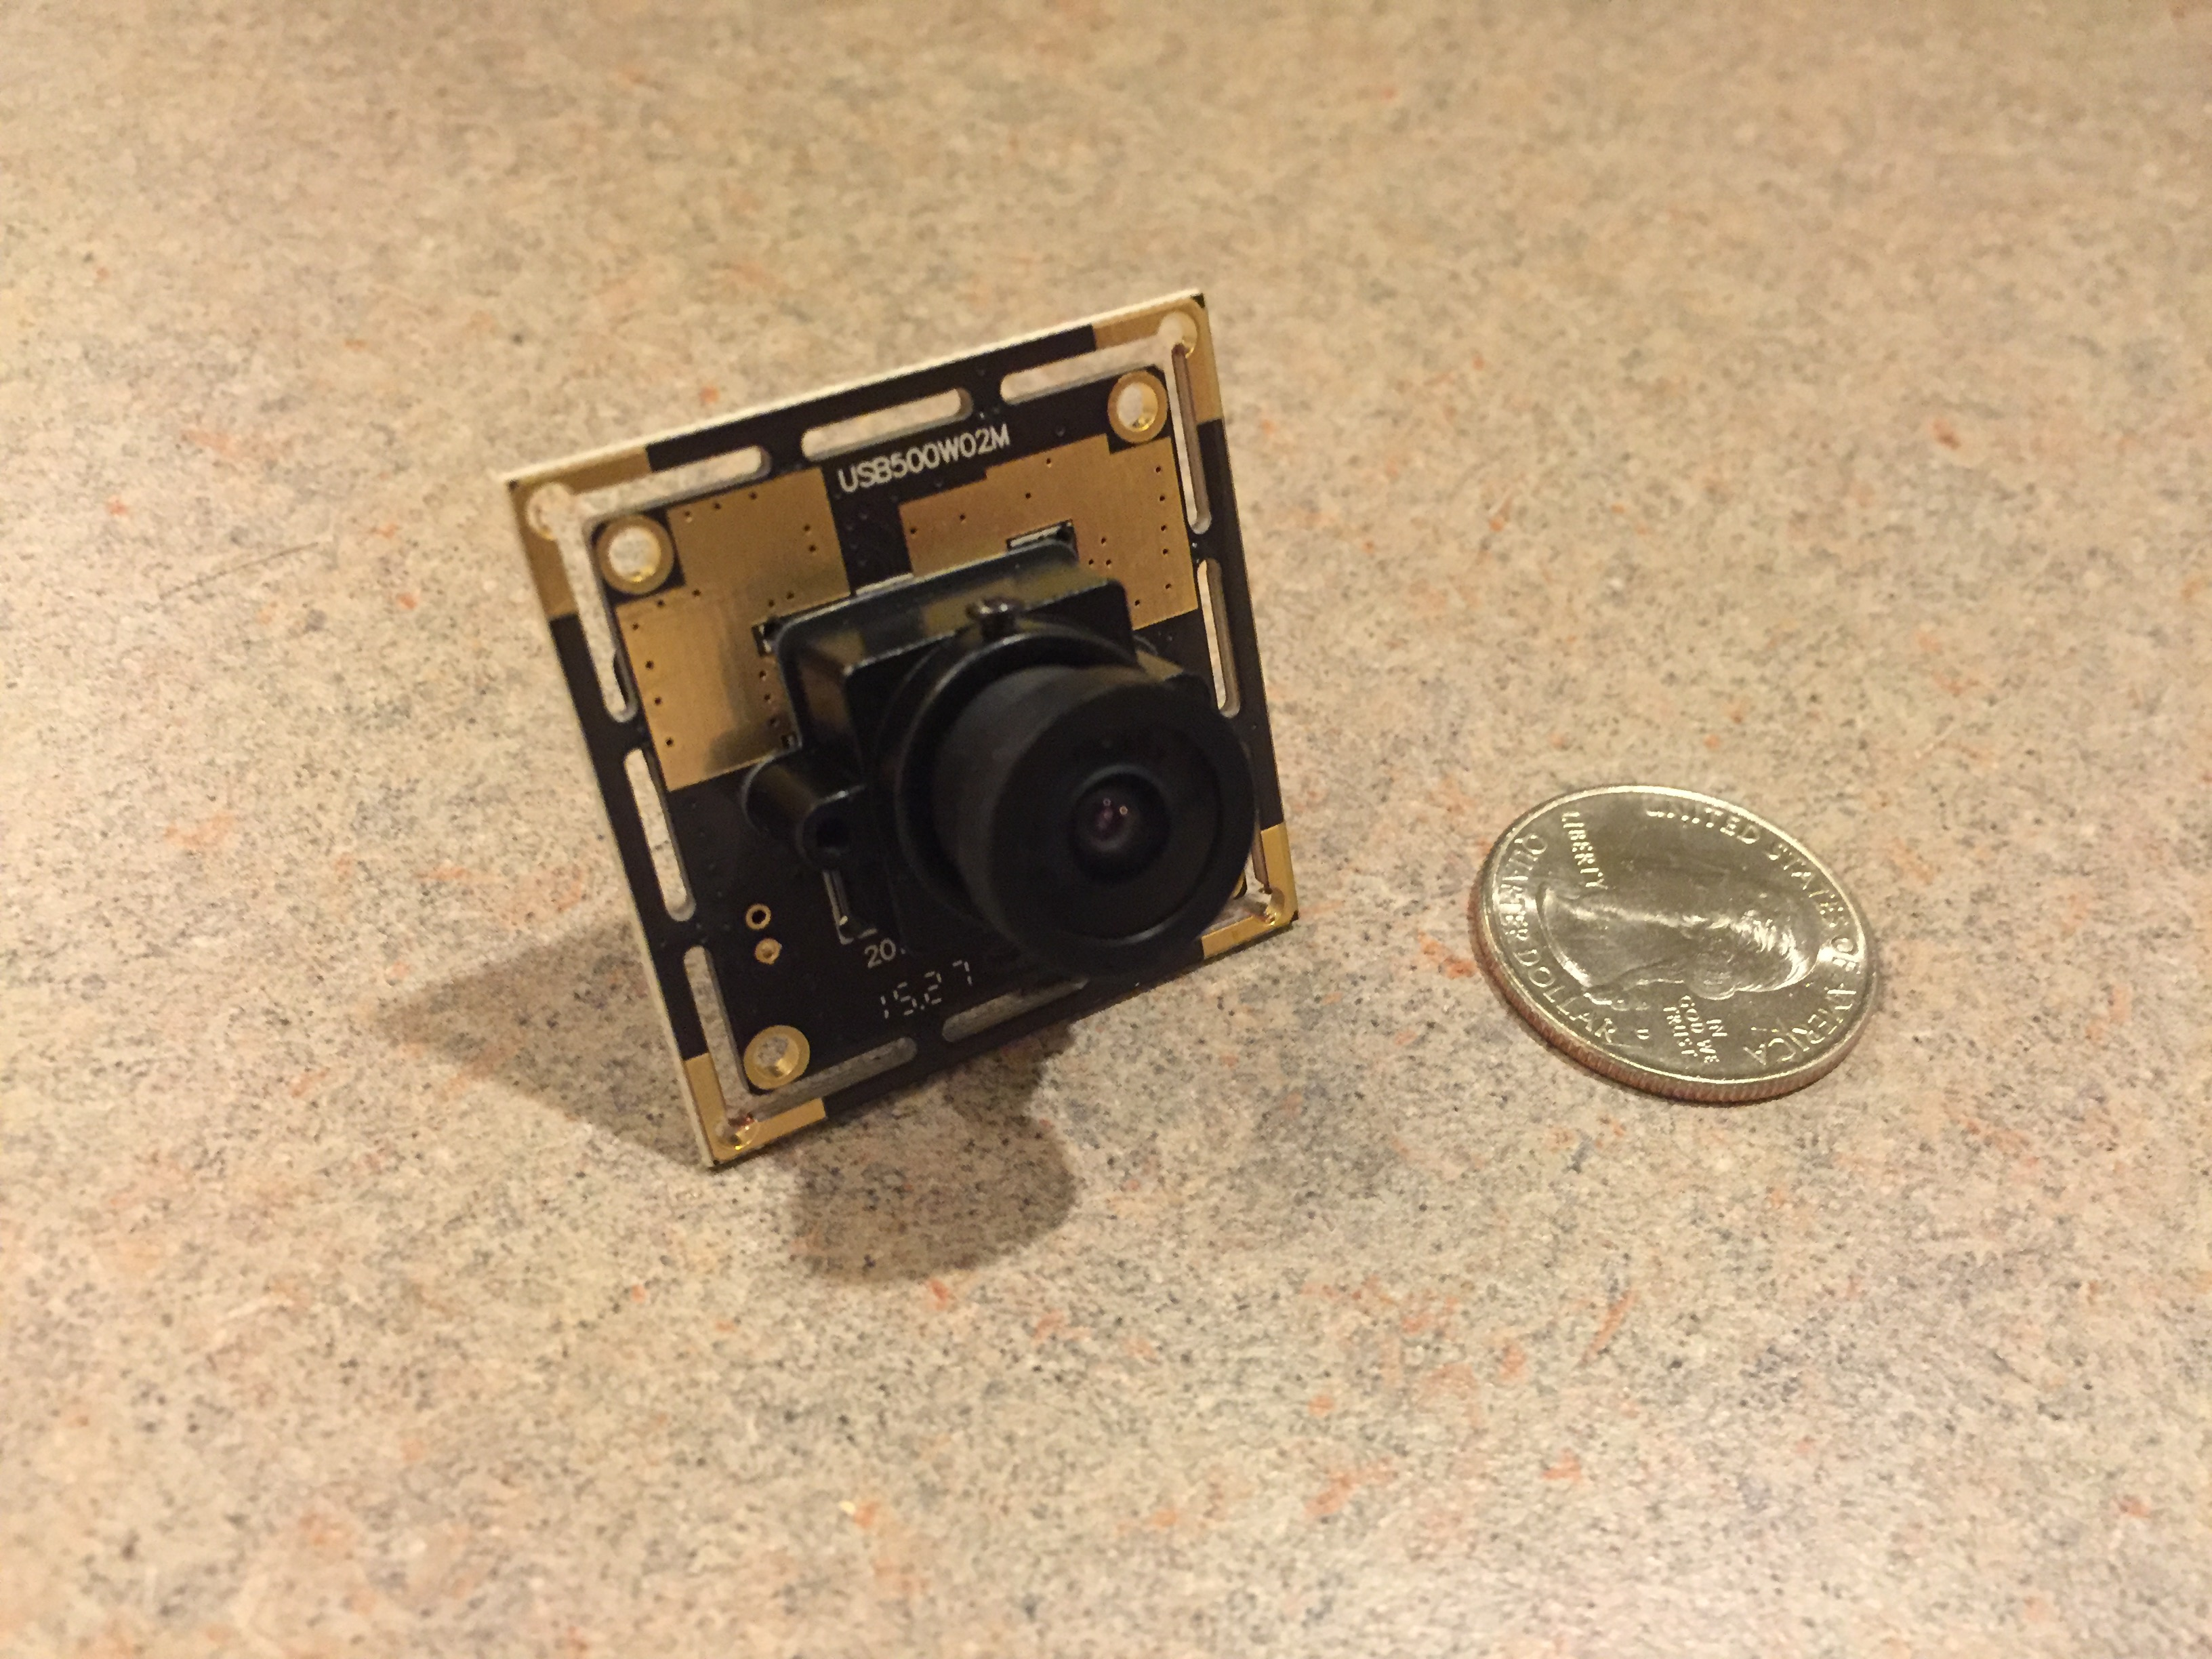
\includegraphics[width=0.5\textwidth]{graphics/camera.jpg}
    \caption{USB Camera}
    \label{fig:camera}
\end{figure}

\subsection{Wireless Communication Interface}

In the quadrotor system, two different communication methods are used. First, in the case of offboard control, bidirectional radio communication is used to exchange messages between a ground control station and the quadrotor, and unidirectional radio communication is used to send inputs from a human user using an RC transmitter. A pair of 3DR Radio V2 kits, developed by 3D Robotics, was used for the bidirectional radio communication, and an AR610 6-channel DSMX Aircraft Receiver, developed by Spektrum, is used for unidirectional communication \cite{radio}\cite{spektrum}. The communication for the ground control station uses 915 MHz frequency and the one for the RC transmitter uses 2.4 GHz frequency.

\begin{figure}
    \centering
    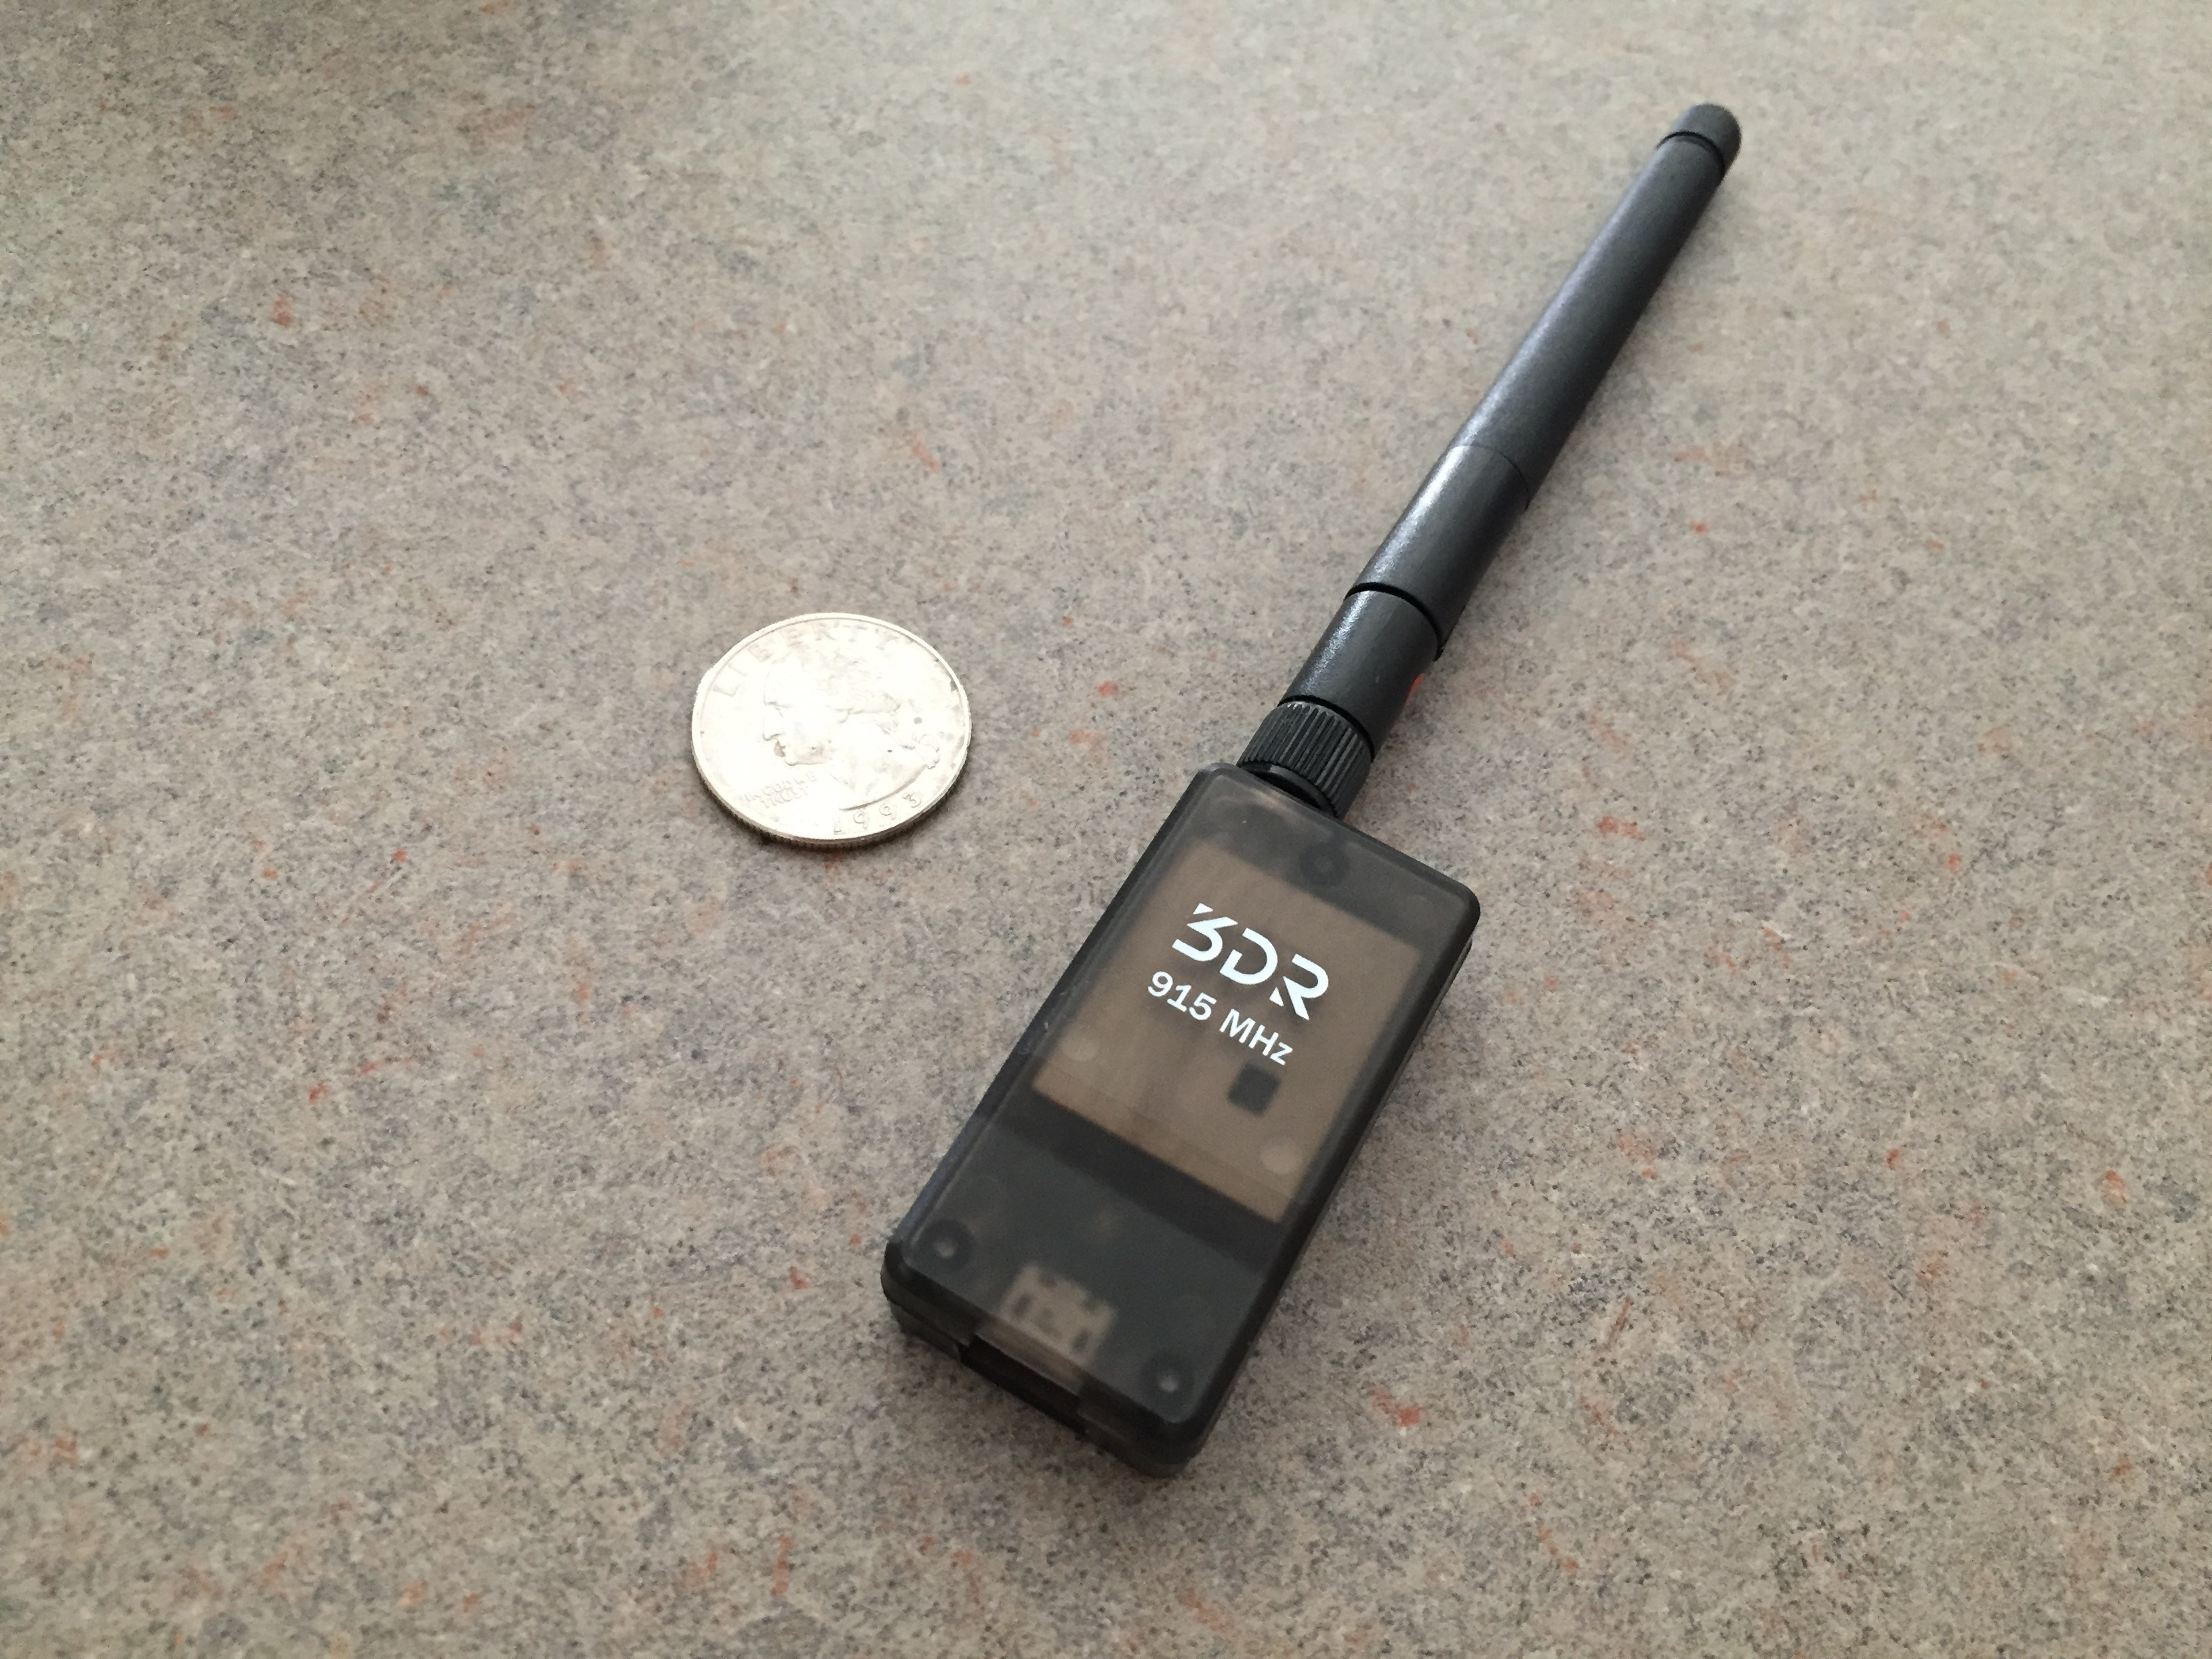
\includegraphics[width=0.5\textwidth]{graphics/telemetry.jpg}
    \caption{3DR radio V2 Telemtery}
    \label{fig:telemetry}
\end{figure}

\begin{figure}
    \centering
    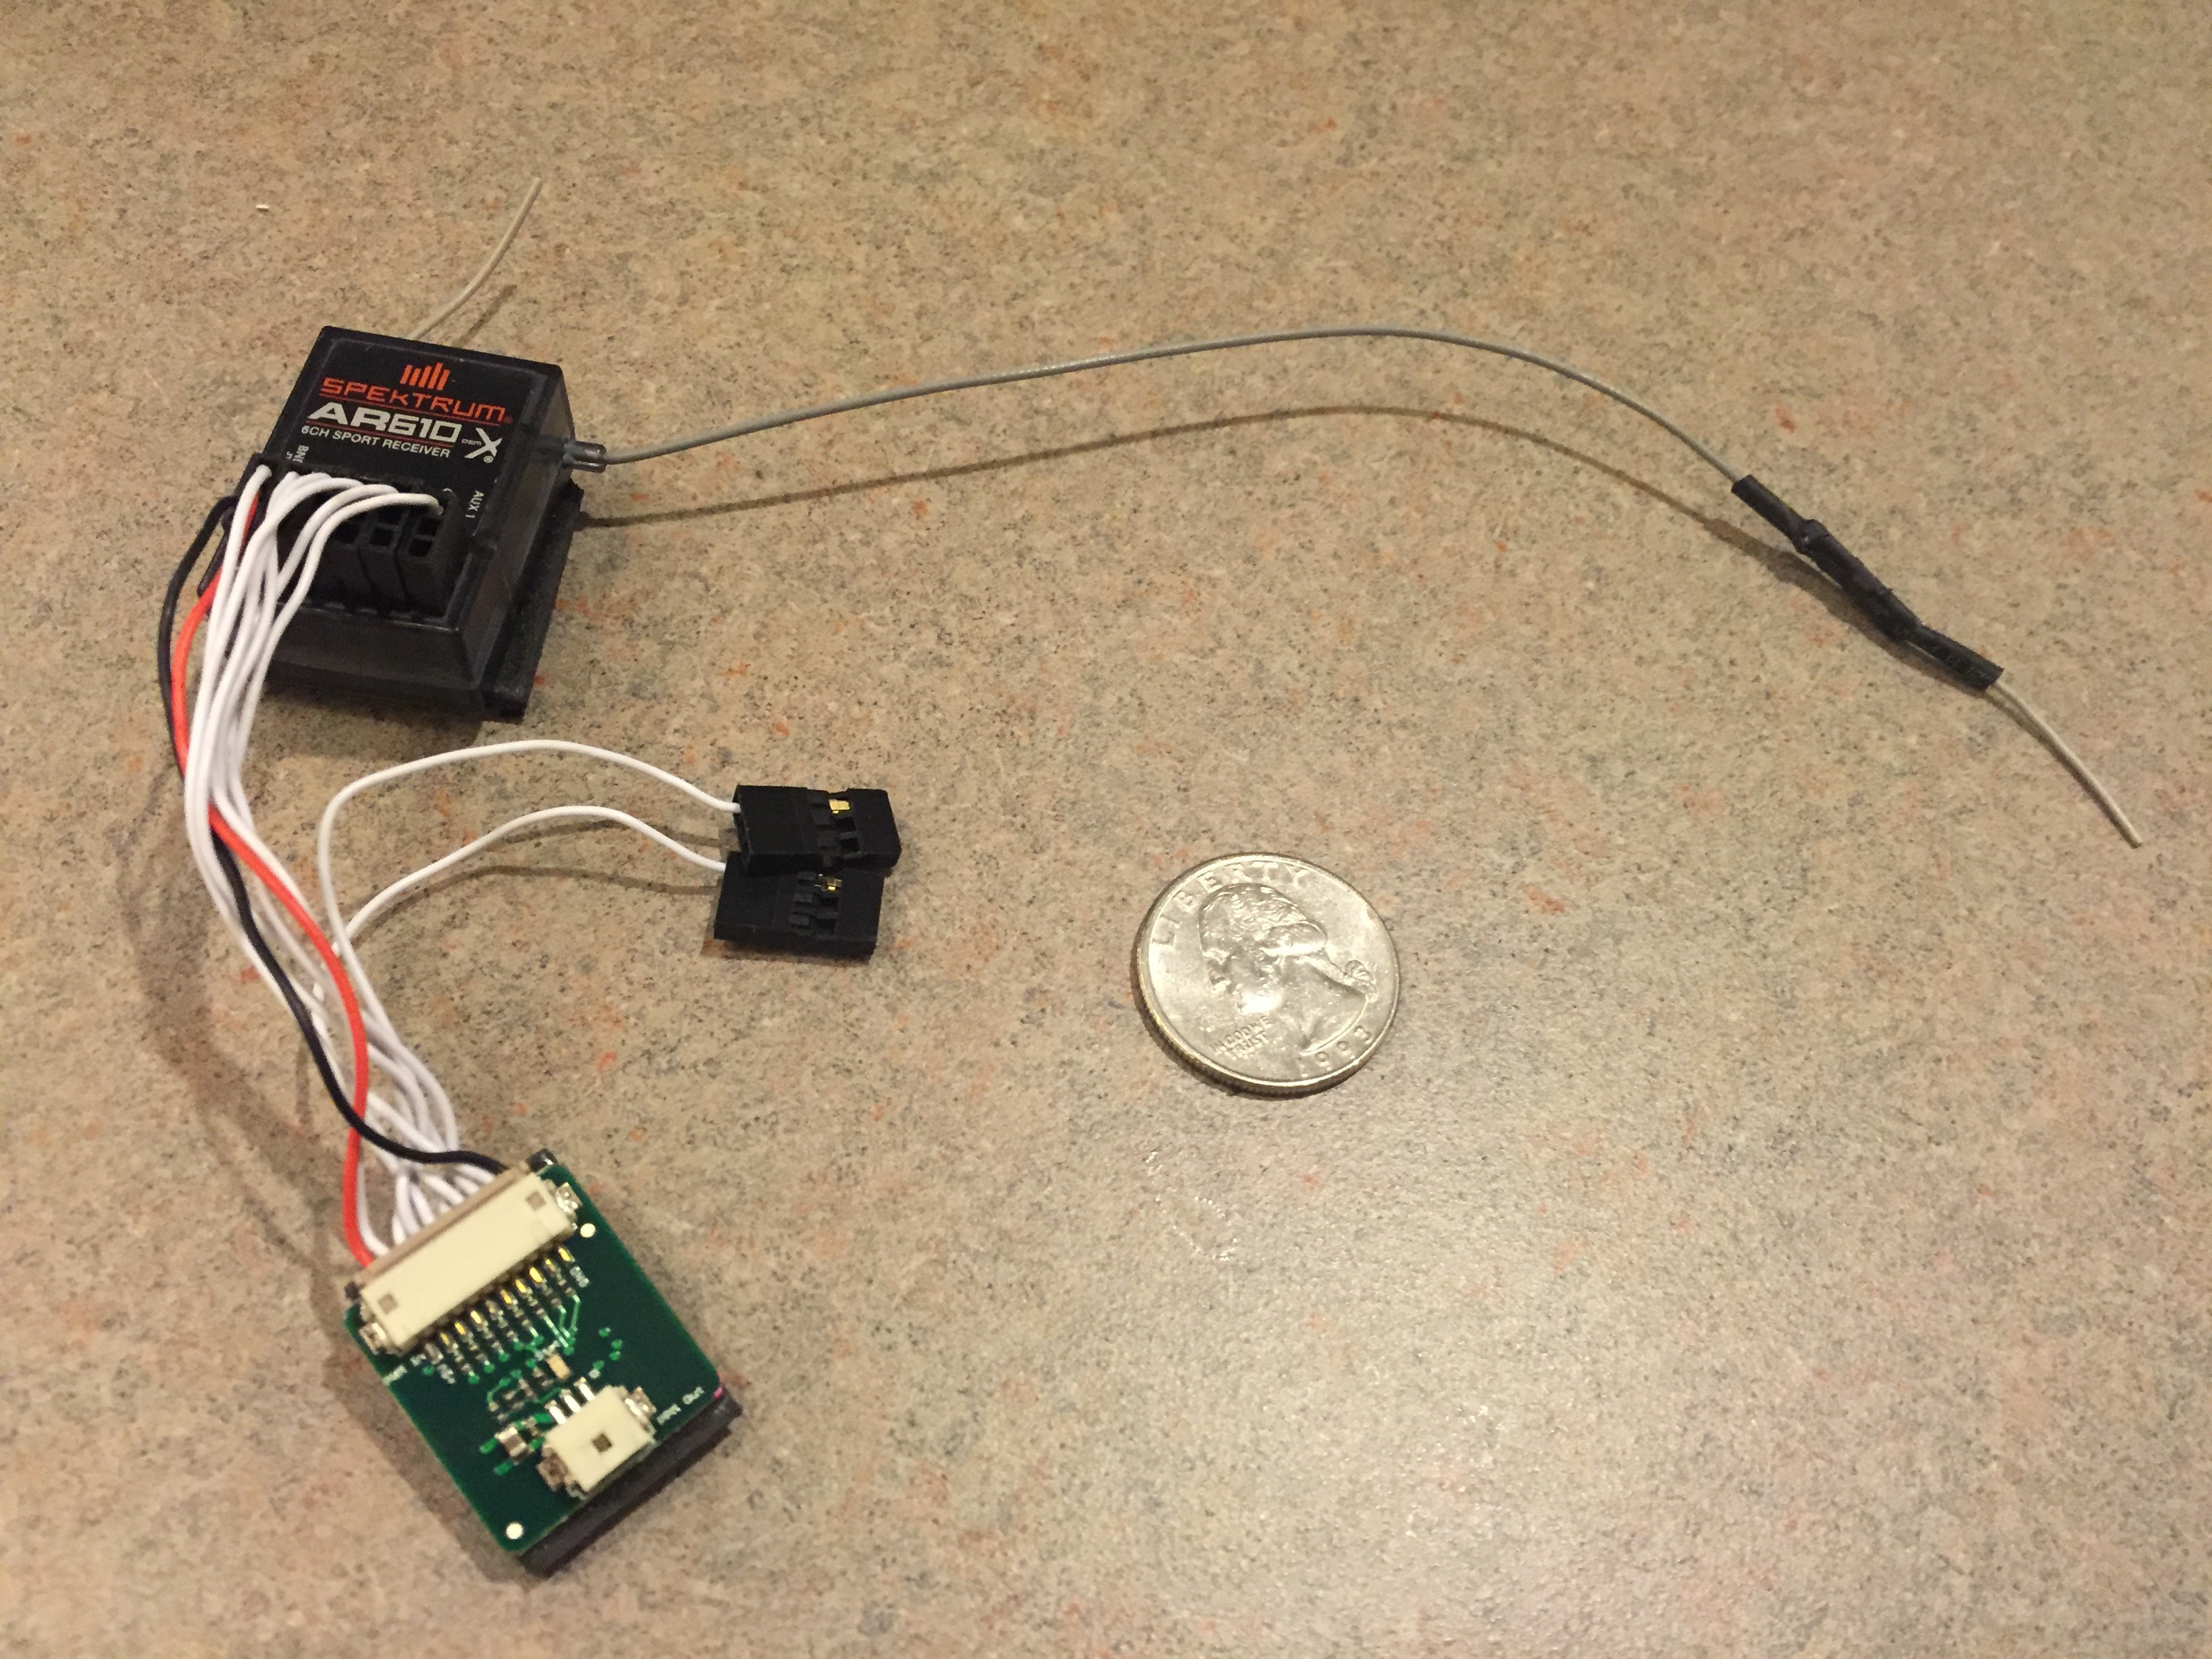
\includegraphics[width=0.5\textwidth]{graphics/rc.jpg}
    \caption{AR610 6-channel DSMX Aircraft Receiver}
    \label{fig:receiver}
\end{figure}

Secondly, in the case of onboard control, messages between the onboard computer and the autopilot are exchanged directly via wired serial communication, and a remote communication interface between the onboard computer and the ground control station is necessary instead. Therefore, a Wi-Fi network is used for communication between the onboard computer and the ground control station. The same communication between the quadrotor and the RC transmitter can be also used as backup. 

\subsection{Ground Control Station}

The ground control station allows us to send commands and receive data remotely. For offboard control, the ground control station must be connected with a radio telemetry with a proper baud rate to receive messages. The telemetry that is connected to the ground station computer must be paired with the one on the quadrotor. 

In the case of onboard control, any computer can be used as a ground control system so long as it is on the same Wi-Fi network since the quadrotor system uses the Wi-Fi network to communicate. The companion computer can be accessed using any wireless interface, such as SSH. Through this interface, a user can use the command console on the onboard companion computer remotely, and the quadrotor's operation can be started.

\section{System Overview}

The complete assembly of the quadrotor is shown in Figure \ref{fig:assemble_01} and \ref{fig:assemble_02}. An overview of the offboard systems of the quadrotor is shown in Figure \ref{fig:overview_01} and one of the onboard system for vision-based estimation is shown in Figure \ref{fig:overview_02}.

\begin{figure}
    \centering
    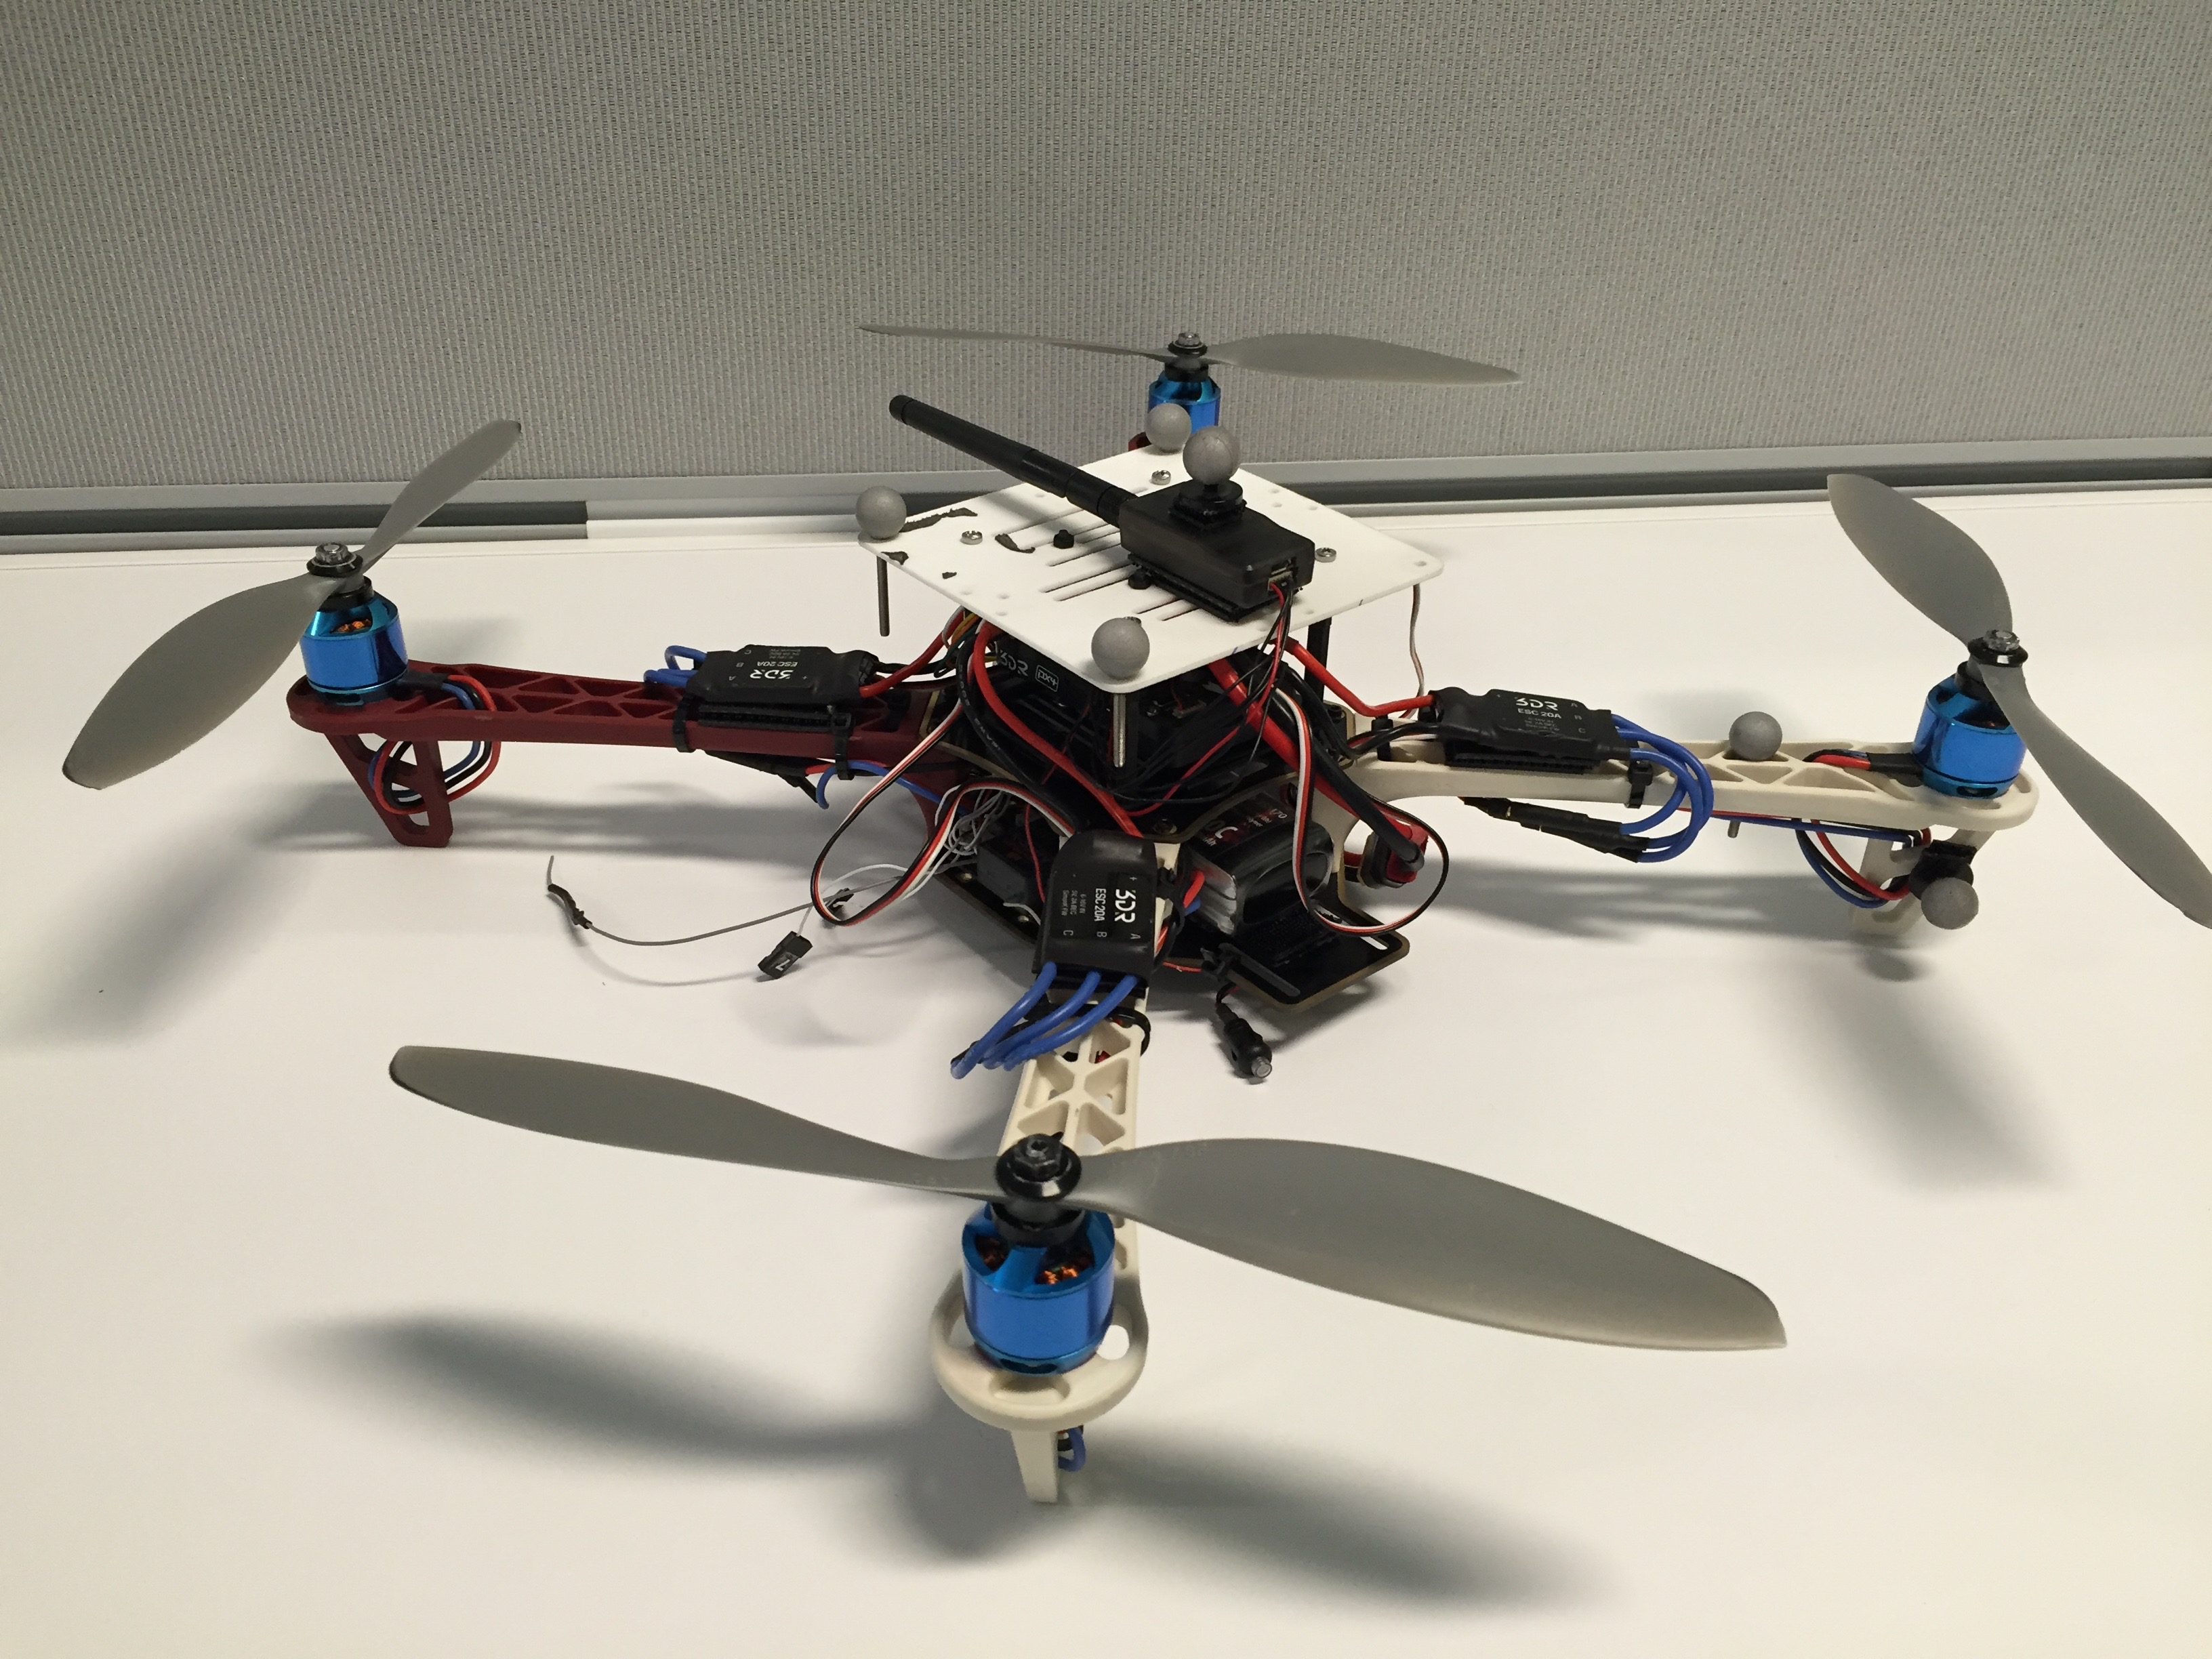
\includegraphics[width=0.8\textwidth]{graphics/quadrotor.jpg}
    \caption{Quadrotor Testbed}
    \label{fig:assemble_01}
\end{figure}

\begin{figure}
    \centering
    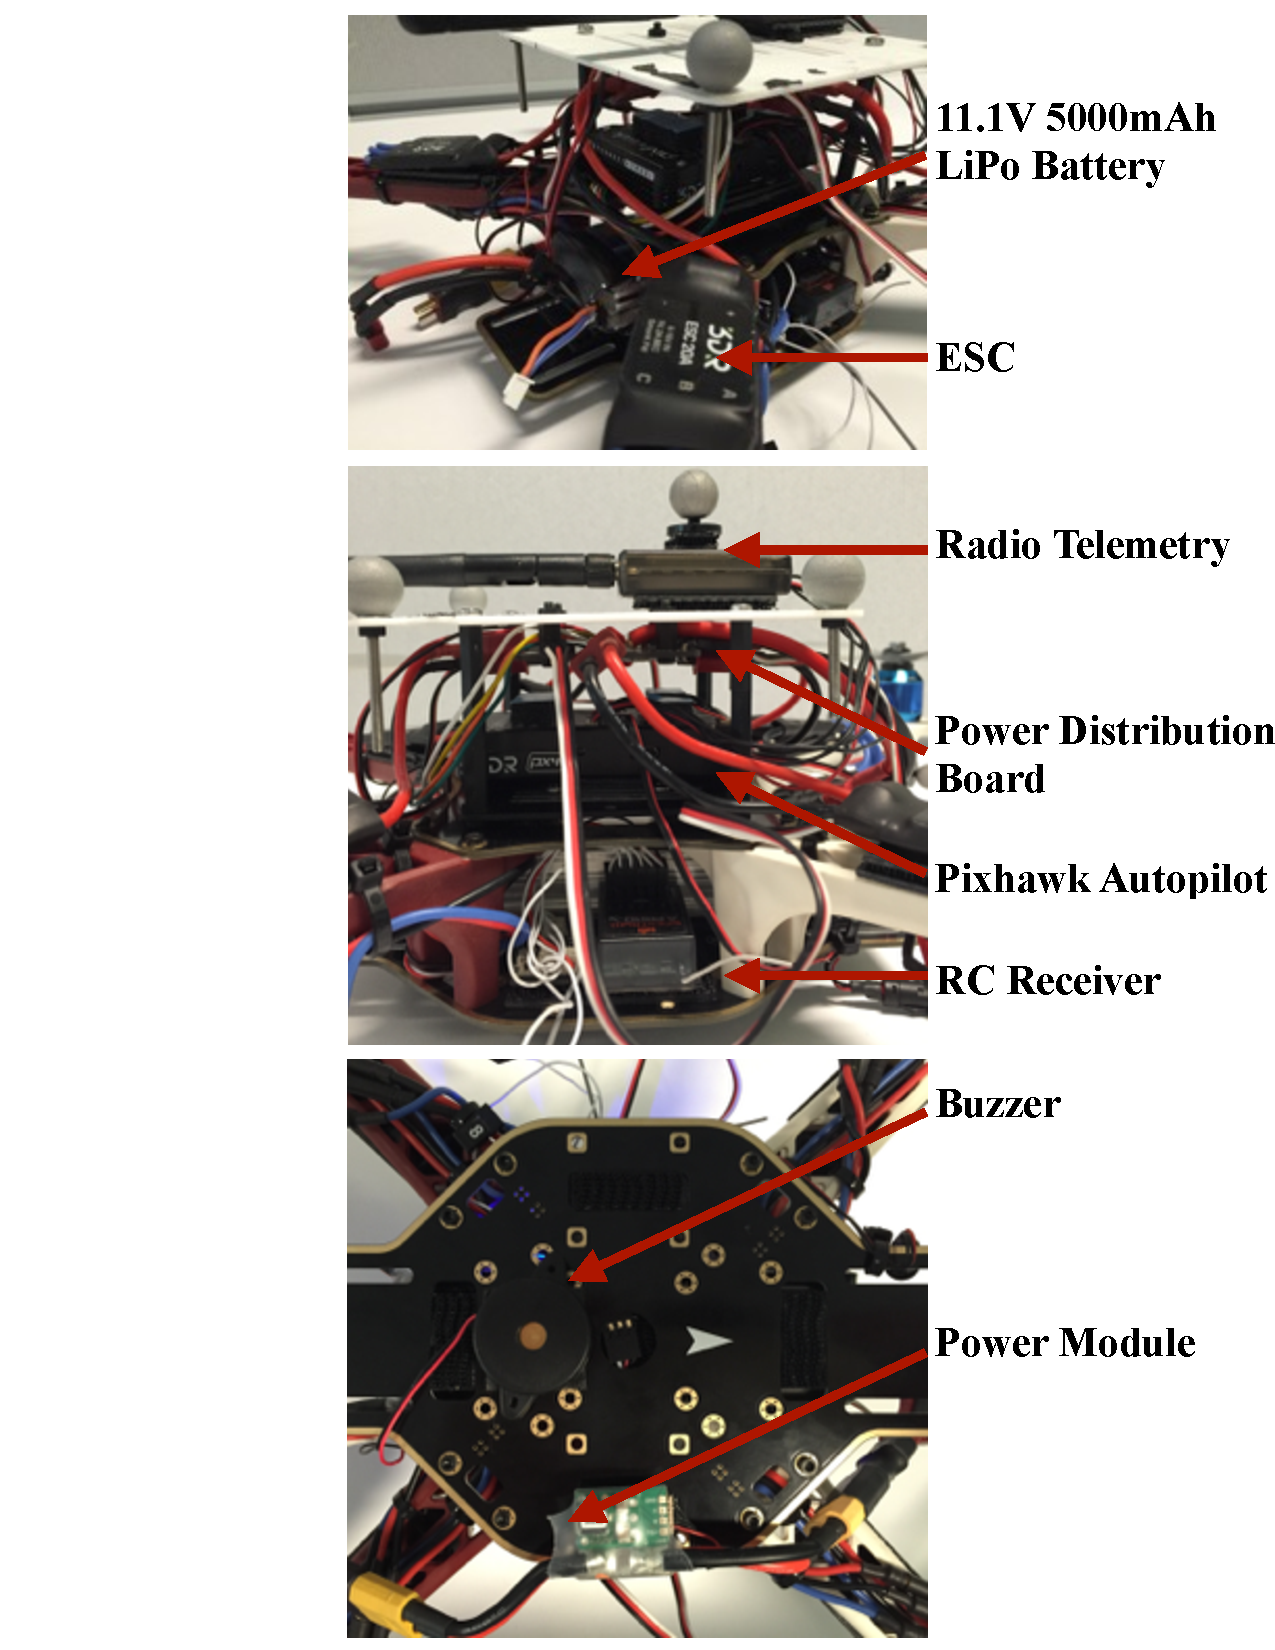
\includegraphics[width=0.9\textwidth]{graphics/hardware.pdf}
    \caption{Description of the Quadrotor Assemble}
    \label{fig:assemble_02}
\end{figure}

\begin{figure}
    \centering
    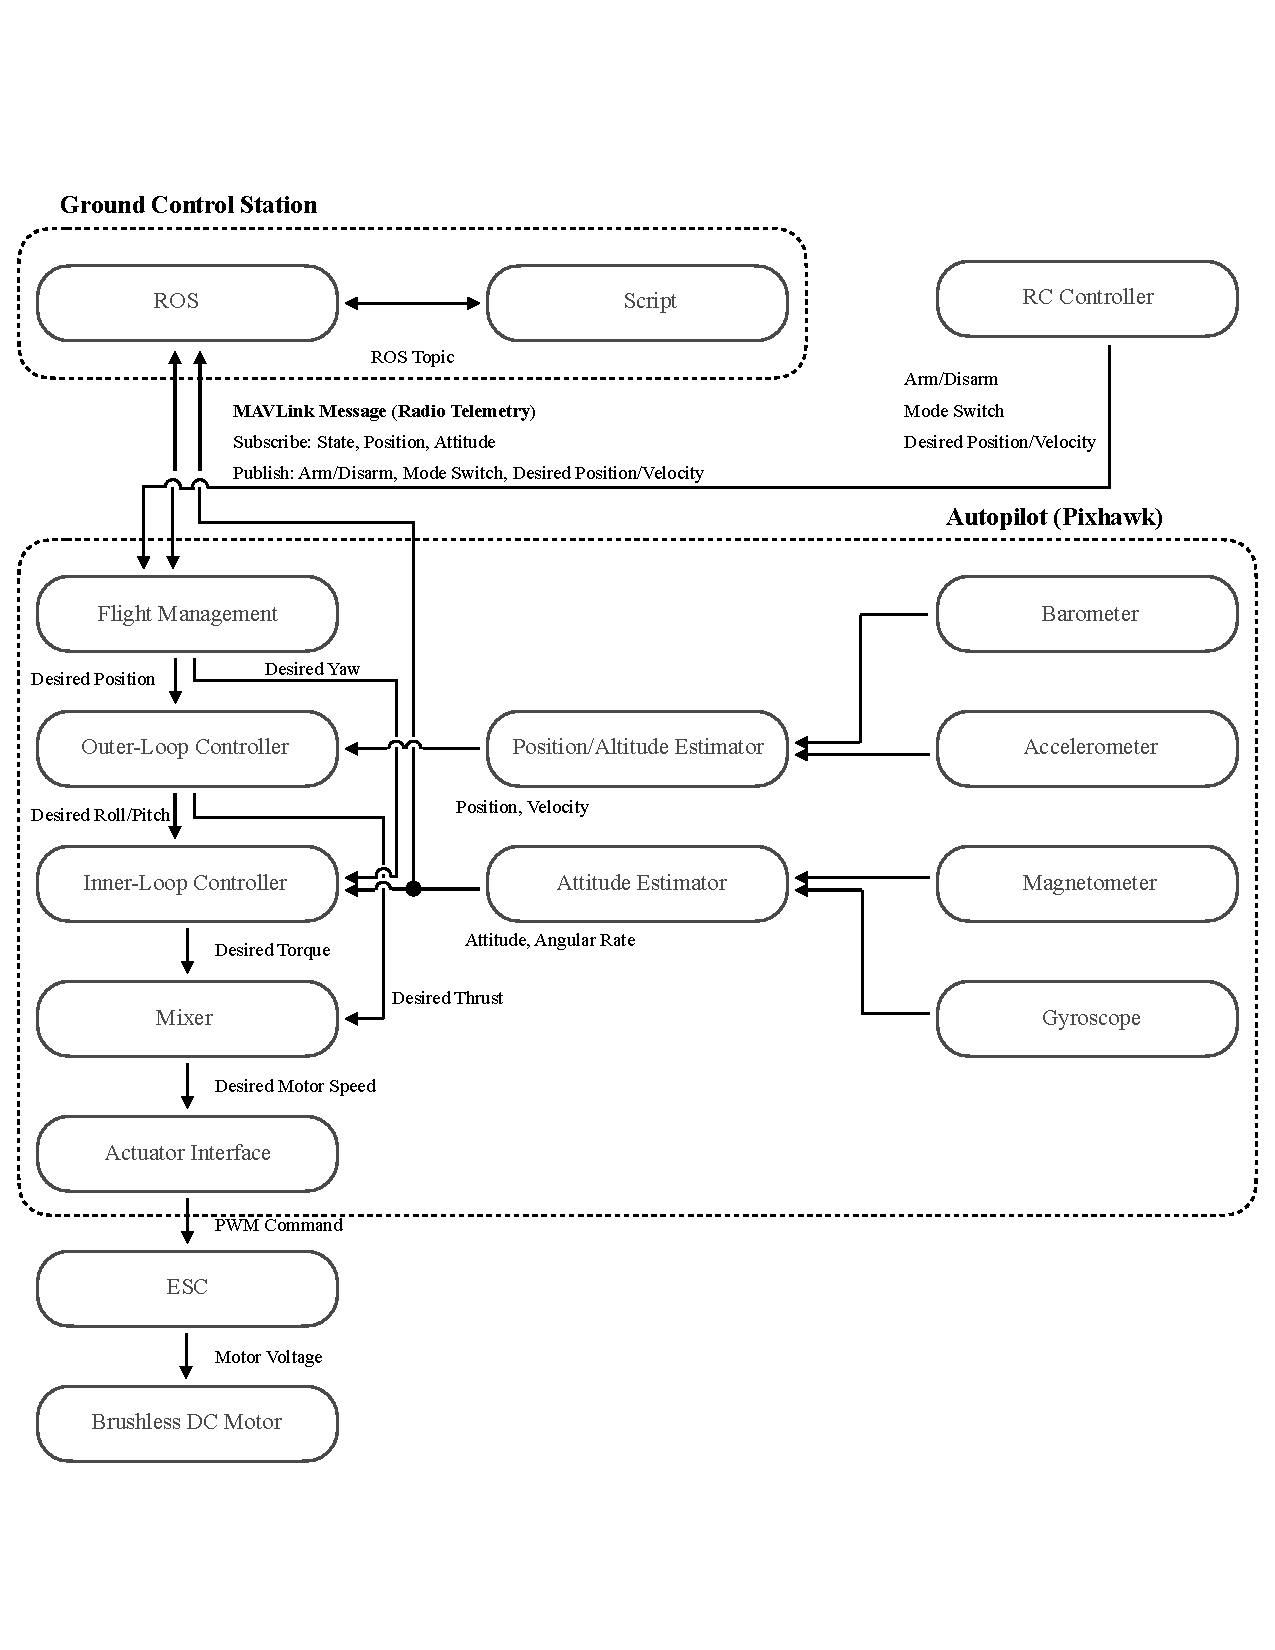
\includegraphics[width=1.0\textwidth]{graphics/architecture_01.pdf}
    \caption{System Architecture of Offboard Control}
    \label{fig:overview_01}
\end{figure}

\begin{figure}
    \centering
    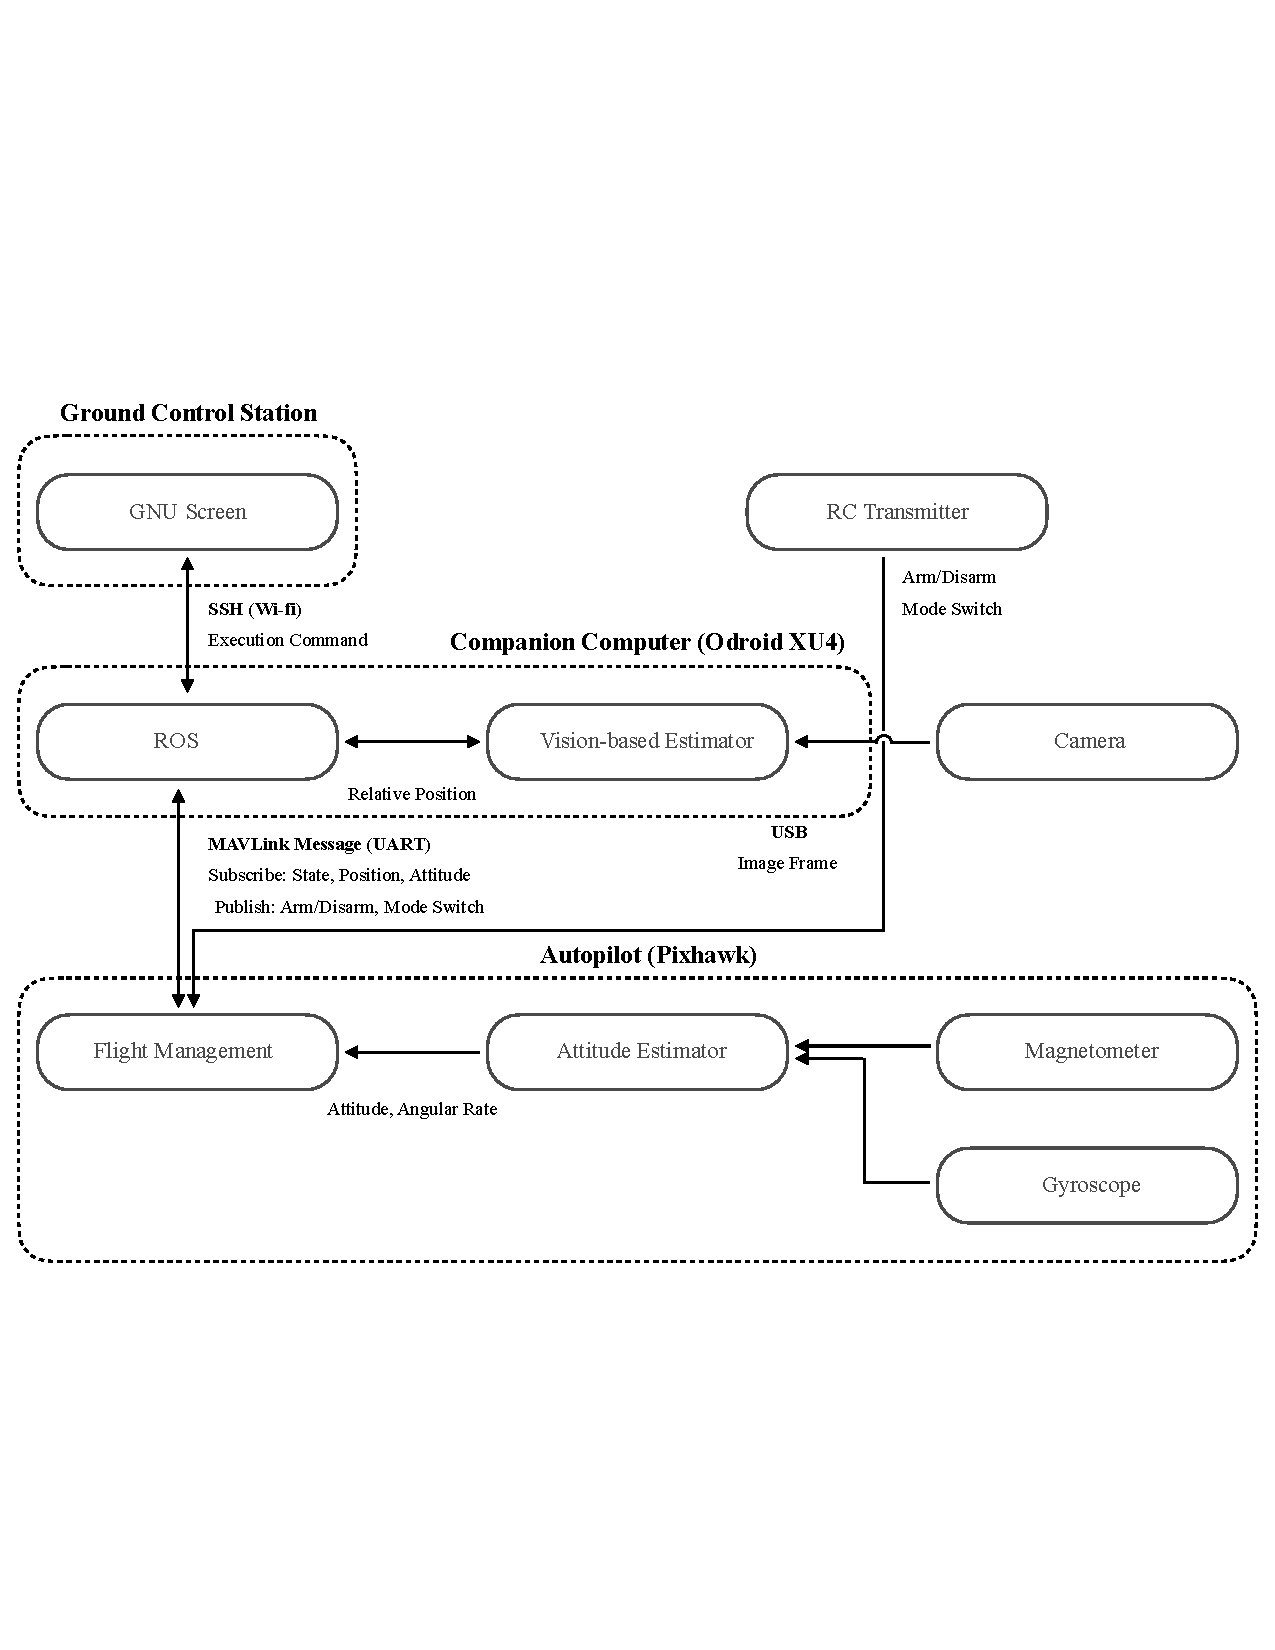
\includegraphics[width=1.0\textwidth]{graphics/architecture_02.pdf}
    \caption{System Architecture of Onboard Control}
    \label{fig:overview_02}
\end{figure}

%%%%%%%%%
In order to operate the quadrotor offboard, the quadrotor must be connected to the ground control station directly through the radio telemetries. A preprogrammed script at the ground control station sends Micro Air Vehicle Link (MAVLink) messages with control commands via radio communication between the radio telemetries stated at Subsection 2.2.8. MAVLink is a protocol that is usually used to communicate UAVs \cite{qgroundcontrol}. MAVROS, a ROS package to deal with MAVLink messages, is used to process MAVLink messages \cite{mavros}. In addition, in order for a human user to send command inputs to the quadrotor, the inputs are sent from the RC transmitter to the RC receiver. The RC receiver is directly connected to the autopilot controller.

On the other hand, the onboard companion computer estimates position information and sends command to the quadrotor, instead of the ground control station. In order to operate the quadrotor onboard, the onboard companion computer must be connected to the ground control station through a Wi-Fi network. Now the companion computer's console is available from the ground control station. Through the GNU SSH interface, the user can start and stop the autonomous operations of the quadrotor. When the autonomous operation starts, the companion computer accesses the autopilot controller and waits until the markers are in view. As soon as the ground facing camera captures the markers, the companion computer starts to estimate the position of the quadrotor. In order to estimate the position, the orientation of the camera must be known. Since the camera is fixed, the quadrotor orientation is same as the orientation of the camera and its information can be measured by the magnetometer of the autopilot. MAVLink messages are used via UART serial communication to communicate between the companion computer and the autopilot. Similar to offboard control, MAVROS is used to deal with MAVLink messages.
%%%%%%%%%
	
Once MAVLink messages are transmitted to the autopilot controller, the remaining tasks are the same in both flight control modes. However, in this research, only offboard control is used for the quadrotor flight, and onboard control is used to evaluate an onboard real-time position measurement. Therefore, the quadrotor both receives maneuver commands and exchanges the quadrotor state information in offboard control, but it only exchanges the state information in onboard control.

	There are multiple modules necessary for quadrotor flight in the autopilot: Inner-loop controller (attitude control), outer-loop controller (position control), position/altitude estimator, attitude control, and mixer. These modules are managed by a flight management system. The quadrotor's orientation, angular, rate, and acceleration are measured by the built in magnetometer, gyroscope, and accelerometer respectively. The quadrotor's position is estimated through the double integration of the acceleration and filters. The estimated altitude is corrected by the built in barometer. However, position in the other two dimensions are not corrected. As the autopilot receives MAVLink messages from the companion computer, the flight management application arms the quadrotor and starts to send setpoint data to the outer-loop controller module. Then, the outer-loop controller computes desired attitude and sends the data to the inner-loop controller module. Continuously, the inner-loop controller module computes desired torques. The mixer module receives the desired torques, computes desired motor speeds, and sends signal to the ESCs to control the motors.
	
	Open loop control is used for motor speed since the DC motors do not have encoders to measure motor speed. Instead, PWM signals are computed according to desired motor speeds to the module of the autopilot. Given PWM signals from the autopilot, each ESC controls the average voltage of its motor, which in turn controls the frequency at which the motor spins.

\section{Physical Properties}
	In order to use the dynamic model of the quadrotor, we need to know the total mass and the moment of inertia. The total mass of the assembled quadrotor is 1.404 kg. The moment of inertia is difficult to measure directly. There are two methods to estimate the moment of inertia: The first is to estimate the moment of inertia from the period of a physical pendulum. The other is to approximate the moment of inertia using a CAD model. Due to the convenience of CAD and the difficulties of installing a precise physical pendulum, we used a CAD model to estimate the moment of inertia. The origin point to compute the moment of inertia is set to be the center of the autopilot controller. The moment of inertia computed by a CAD model is given as below,\\
\begin{equation}
\begin{aligned}
J & = 
\begin{bmatrix}
J_{xx} & J_{xy} & J_{xz} \\
J_{xy} & J_{yy} & J_{yz} \\
J_{xz} & J_{yz} & J_{zz}
\end{bmatrix}\\
& = 
\begin{bmatrix}
1.206 & - 0.003318 & -0.008680 \\
- 0.003318 & 1.285 & -0.001466 \\
-0.008680 & -0.001466 & 2.347
\end{bmatrix}
\times {10}^{-2} [\textstyle{kg} {\textstyle{m}}^2]\\
\end{aligned}
\end{equation}
The diagonal elements \(J_{xx}\), \(J_{yy}\), \(J_{zz}\) are at least 150 times greater than any cross moments of inertia, the moment of inertia \(J\) is approximated as a positive diagonal matrix.\\
\begin{equation}
\begin{aligned}
J & \approx 
\begin{bmatrix}
1.206 & 0 & 0 \\
0 & 1.285 & 0 \\
0 & 0 & 2.347
\end{bmatrix}
\times {10}^{-2} [\textstyle{kg} {\textstyle{m}}^2]\\
\end{aligned}
\end{equation}
This implies that the quadrotor has a nearly symmetric structure about all axises. The components that have comparatively great mass, such as DC motors, are installed symmetrically. Even if the components that have small mass, such as the radio telemetry, are located asymmetrically, they have little effect on the moment of inertia. In addition, the battery is set close to the center of inertia, so its effect on the moment of inertia is expected to be small.

\begin{figure}
    \centering
    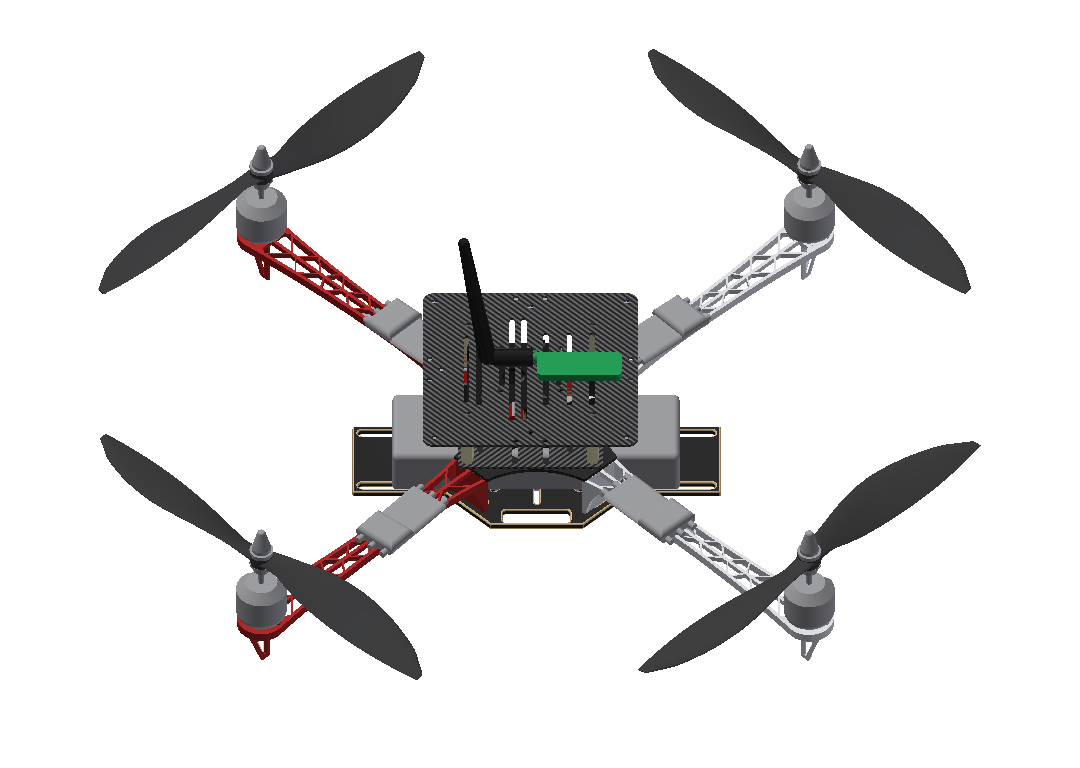
\includegraphics[width=0.6\textwidth]{graphics/cad_upper.png}
    \caption{CAD model of the Quadrotor (upper side)}
    \label{fig:cad_1}

\vspace{1cm}
    \centering
    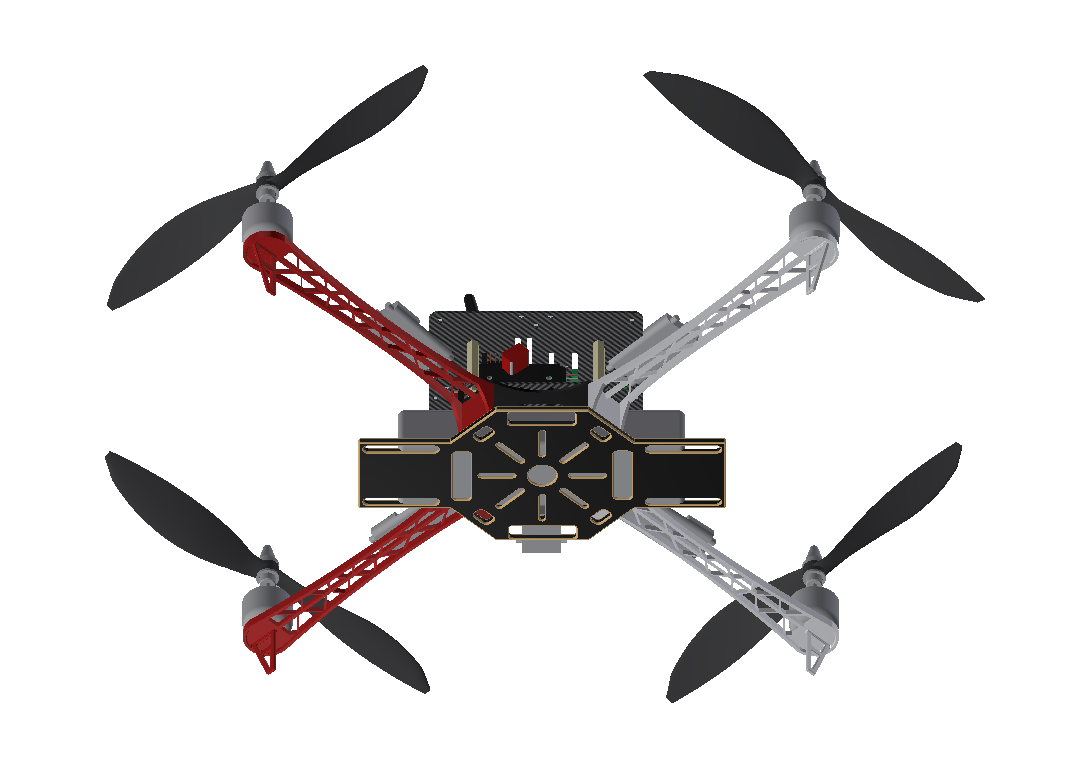
\includegraphics[width=0.6\textwidth]{graphics/cad_under.png}
    \caption{CAD model of the Quadrotor (under side)}
    \label{fig:cad_2}
\end{figure}




\chapter{Control System}
\label{ch:control_system}

The control system is one of the most important parts in the quadrotor's operation. In this research, we implemented a nonlinear attitude control system based on a dynamic model of the quadrotor. In this chapter, coordinate systems for the quadrotor's control are defined, the dynamic model of the quadrotor is introduced, and the control system is described.

\section{Control System Overview}
\label{sec:control_system_system_overview}

The overview of the control system is illustrated in Figure \ref{fig:bode}. First, the outer-loop controller receives desired position and desired attitude. Then, the outer-loop controller receives current state data from the sensors, and computes desired attitude and thrust corresponding to position errors of the quadrotor. The current position is estimated by synchronization of the internal accelerometer and barometer sensors, and other external sensors, such as a camera and a motion capture system. The inner-loop controller receives the quadrotor's attitude and angular velocity from the onboard gyroscope and magnetometer, and computes desired torque to control the attitude. The quadrotor's current attitude is measured by the internal magnetometer and angular velocity is measured by the internal gyroscope. Finally, the mixer, an open-loop motor controller, receives the desired thrust from the outer-loop controller and the desired torque from the inner-loop controller. Then, the mixer maps the desired thrust and torque into desired motor speeds, and estimates desired voltage of each motor.

\begin{figure}
    \centering
    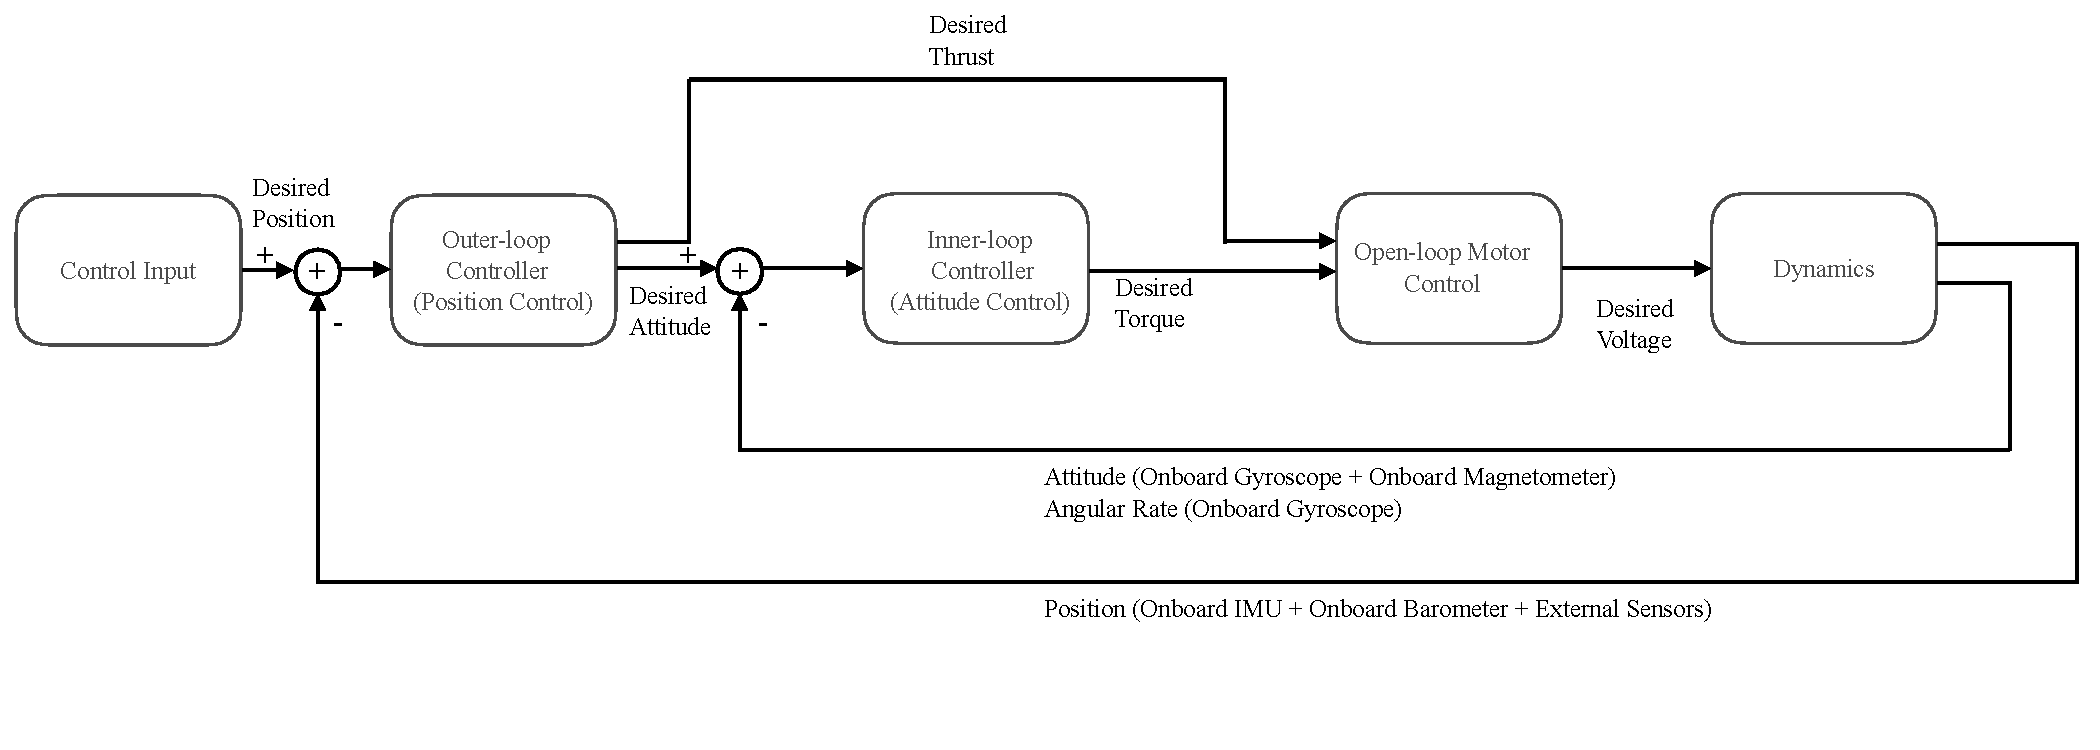
\includegraphics[width=1\textwidth]{graphics/bode_diagram.pdf}
    \caption{Illustration of the Control System.}
    \label{fig:bode}
\end{figure}

\section{Coordinate System}
\label{sec:coordinate_system}

In order to control the motion and state of the quadrotor, coordinate systems must be defined for the state and motion representation.\cite{intro_to_robotics} %john craig
First, a reference coordinate system must be defined to describe the orientation and position of the quadrotor. The reference coordinate system is called an "inertial coordinate system". Commonly, an inertial coordinate system is defined to be a Cartesian coordinate system that has its x, y-plane fixed on the ground. For convenience of control, the z-axis of the quadrotor is defined to face the ground. The origin can be arbitrarily set, but it is defined to be the initial position of the quadrotor in this research. 

In addition, it helps description of the quadrotor's motion to define a body-attached coordinate system since the onboard sensors of the quadrotor are fixed on the quadrotor's frame. In the quadrotor system, the body coordinate system follows the convention; the x, y-axises are defined to be parallel to the quadrotor's frame, and the z-axis is defined to be downward. The origin is set to be at the center of the autopilot controller, approximately at the center of mass.

\begin{figure}
    \centering
    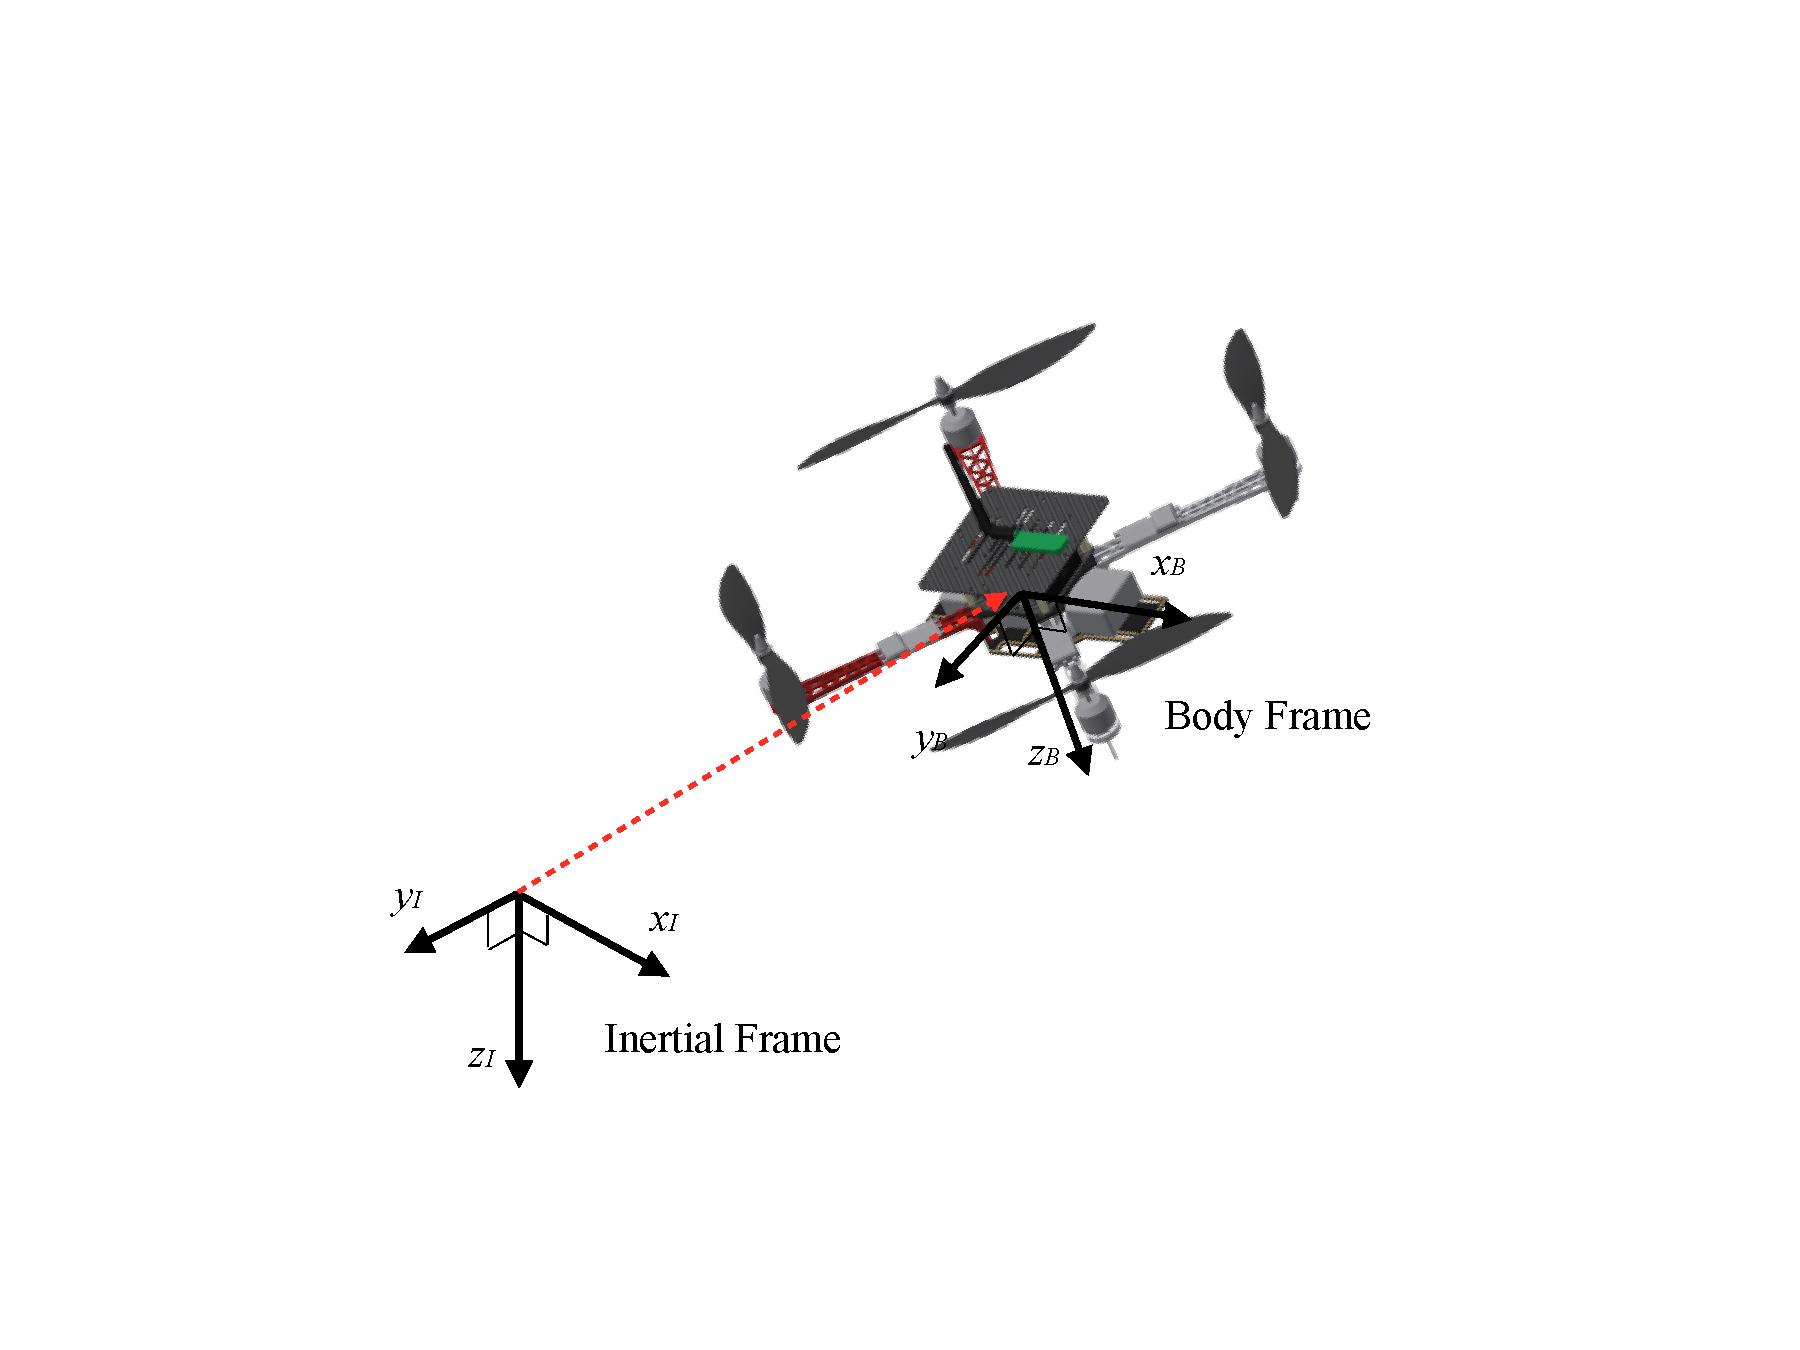
\includegraphics[width=0.8\textwidth]{graphics/coordinate.pdf}
    \caption{Illustration of the Inertial and Body Frames.}
    \label{fig:frame}
\end{figure}

Using the above coordinate systems, the quadrotor motion is represented completely. The mapping of the origin in the body frame into the inertial frame represents the quadrotor position. The orientation of the body frame is represented by multiple methods, such as the X-Y-Z fixed angles convention and the Z-Y-X Euler angles convention. In this research, the Z-Y-X Euler angles convention, also known as the Tait-Bryan angles convention, is used \cite{Diebel06}. In the Z-Y-X Euler angle convention, the mapping into the body frame starts with rotating about the z-axis by a yaw angle \(\psi\). Rotation of the y-axis by a pitch angle \(\theta\), and the z-axis by a roll angle \(\phi\) are followed in order. The transformation matrix of an orientation from the body frame into the inertial frame is given as,\\
\begin{equation}
\label{eq:transform_matrix}
\begin{aligned}
{^I _B}R
& = {R_{z, \psi}}  {R_{y, \theta}} {R_{x, \phi}}\\
& =
\begin{bmatrix}
\cos{\psi} & -\sin{\psi} & 0 \\
\sin{\psi} & \cos{\psi} & 0\\
0 & 0 & 1
\end{bmatrix}
\begin{bmatrix}
\cos{\theta} & 0& \sin{\theta} \\
0 & 1 & 0 \\
-\sin{\theta} & 0 & \cos{\theta}
\end{bmatrix}
\begin{bmatrix}
1 & 0 & 0\\
0& \cos{\phi} & -\sin{\phi} \\
0 & \sin{\phi} & \cos{\phi} \\
\end{bmatrix}\\
& =
\begin{bmatrix}
\cos{\theta} \cos{\psi} & \sin{\phi} \sin{\theta} \cos{\psi} - \cos{\phi}\sin{\psi} & \cos{\phi} \sin{\theta} \cos{\psi} + \sin{\phi} \sin{\psi}\\
\cos{\theta} \sin{\psi} & \sin{\phi} \sin{\theta} \sin{\psi} + \cos{\phi}\cos{\psi} & \cos{\phi} \sin{\theta} \sin{\psi} - \sin{\phi} \cos{\psi}\\
-\sin{\theta} &  \sin{\phi} \cos{\theta} & \cos{\phi} \cos{\theta}
\end{bmatrix}\\
\end{aligned}
\end{equation}
and the inverse transformation is given as,\\
\begin{equation}
\begin{aligned}
{^B _I}R
& = {{^B _I}R}^{-1}\\
& = {R_{x, \phi}}^{T}  {R_{y, \theta}}^{T} {R_{z, \psi}}^{T}\\
&=
\begin{bmatrix}
1 & 0 & 0\\
0& \cos{\phi} & \sin{\phi} \\
0 & - \sin{\phi} & \cos{\phi} \\
\end{bmatrix}
\begin{bmatrix}
\cos{\theta} & 0& - \sin{\theta} \\
0 & 1 & 0 \\
\sin{\theta} & 0 & \cos{\theta}
\end{bmatrix}
\begin{bmatrix}
\cos{\psi} & \sin{\psi} & 0 \\
-\sin{\psi} & \cos{\psi} & 0\\
0 & 0 & 1
\end{bmatrix}\\
& =
\begin{bmatrix}
  \cos{\theta} \cos{\psi}  &  \cos{\theta} \sin{\psi} & - \sin{\theta}  \\
\sin{\phi} \sin{\theta} \cos{\psi} - \cos{\phi} \sin{\psi} & \sin{\phi} \sin{\theta} \sin{\psi} + \cos{\phi} \cos{\psi} & \sin{\phi} \cos{\theta} \\
\cos{\phi} \sin{\theta} \cos{\psi}  +  \sin{\phi} \sin{\psi} & \cos{\phi} \sin{\theta} \sin{\psi}- \sin{\phi} \cos{\psi} & \cos{\phi}\cos{\theta}
\end{bmatrix}\\
\end{aligned}
\end{equation}

\section{Outer-Loop Controller}
\label{sec:outer_loop}

The outer-loop controller calculates desired attitude of the quadrotor, based on a given desired position and the quadrotor's current position. As a method of controlling the position of the quadrotor, PID control is applied. In this section, the outer-loop controller will be introduced. First, dynamics with respect to the quadrotor's position is described. Then, the position control of the quadrotor is stated.

\subsection{Dynamics Description}

A quadrotor is accelerated by thrust generated by its four rotors. Let \( {\boldsymbol F} = (\overline{X}, \overline{Y}, \overline{Z})\) be the quadrotor's thrust specified in the inertial frame. Then, the equation of motion is given as,
\begin{equation}
\label{eq:newton}
\begin{aligned}
m \ddot{{\boldsymbol{r}}} = \boldsymbol{F} + m \boldsymbol{g}\\
\end{aligned}
\end{equation}
where \(m\) is the mass of the quadrotor, \({\boldsymbol r} = (x, y, z)\) is the position of the quadrotor in the inertial frame, and \(\boldsymbol{g} = (0, 0, -g)\) is the gravitational acceleration.

Since the rotation axis of each rotor is fixed perpendicularly to the body, thrust can be generated only in the perpendicular direction of the body frame. Therefore, thrust can be computed by a rotation transformation from the body frame into the inertial frame. From equation (\ref{eq:transform_matrix}), thrust vector in the inertial frame is given as,
\begin{equation}
\begin{aligned}
{\boldsymbol F}
& = {^I_B}{R} 
\begin{bmatrix}
0\\
0\\
F
\end{bmatrix}\\
& =
\begin{bmatrix}
\cos{\theta} \cos{\psi} & \sin{\phi} \sin{\theta} \cos{\psi} - \cos{\phi}\sin{\psi} & \cos{\phi} \sin{\theta} \cos{\psi} + \sin{\phi} \sin{\psi}\\
\cos{\theta} \sin{\psi} & \sin{\phi} \sin{\theta} \sin{\psi} + \cos{\phi}\cos{\psi} & \cos{\phi} \sin{\theta} \sin{\psi} - \sin{\phi} \cos{\psi}\\
-\sin{\theta} &  \sin{\phi} \cos{\theta} & \cos{\phi} \cos{\theta}
\end{bmatrix}
\begin{bmatrix}
0\\
0\\
F
\end{bmatrix}\\
& =
F
\begin{bmatrix}
\cos{\phi} \sin{\theta} \cos{\psi} + \sin{\phi} \sin{\psi}\\
\cos{\phi} \sin{\theta} \sin{\psi} - \sin{\phi} \cos{\psi}\\
\cos{\phi} \cos{\theta}\\
\end{bmatrix}
\end{aligned}
\end{equation}
where \( F = \sqrt{{\overline{X}}^2 + {\overline{Y}}^2 + {\overline{Z}}^2}\) is the magnitude of the thrust, and \( {\boldsymbol \eta} = (\phi, \theta, \psi) \) is the attitude (roll, pitch, and yaw, respectively) of the quadrotor. Then, the thrust along each axis of the inertial frame is given as,
\begin{equation}
\label{eq:thrust_vector}
\begin{aligned}
{\overline X} &=  F (\cos{\phi} \sin{\theta} \cos{\psi} + \sin{\phi} \sin{\psi})\\
{\overline Y} &= F (\cos{\phi} \sin{\theta} \sin{\psi} - \sin{\phi} \cos{\psi})\\
{\overline Z} &=  F \cos{\phi} \cos{\theta}\\
\end{aligned}
\end{equation}
Therefore, from Equations (\ref{eq:newton}) and (\ref{eq:thrust_vector}), the acceleration of the quadrotor \({(\ddot{x}}, {\ddot{y}}, {\ddot{z}})\) is computed as,
\begin{equation}
\begin{aligned}
{{\ddot x} } & =  {F \over m} (\cos{\phi} \sin{\theta} \cos{\psi} + \sin{\phi} \sin{\psi})\\
{{\ddot y} } & =  {F \over m} (\cos{\phi} \sin{\theta} \sin{\psi} - \sin{\phi} \cos{\psi})\\
{{\ddot z} } & =  {F \over m} \cos{\phi} \cos{\theta} -g\\
\end{aligned}
\end{equation}

The sensors are fixed on the quadrotor, and therefore, it is necessary to formulate the relation of the quadrotor motion in the body frame and the inertial frame. Let \({\boldsymbol v}_B = (u, v, w)\) be the quadrotor's velocity in the body frame and \({\boldsymbol \omega} = (p, q, r)\) be the quadrotor's angular velocity. From the Coriolis effect, the equation of motion is given with respect to \( {\boldsymbol v}_B \) as the below equation \cite{randal08}.
\begin{equation}
\label{eq:newton_gravity}
\begin{aligned}
m \ddot{{\boldsymbol{r}}} = m (\dot{{\boldsymbol v}}_B + {\boldsymbol \omega} \times {\boldsymbol v}_B)\\
\end{aligned}
\end{equation}
Hence, from Equation (\ref{eq:newton}) the equation of the quadrotor's thrust \({\boldsymbol F}\) is written as,
\begin{equation}
\begin{aligned}
\boldsymbol{F} = m (\dot{{\boldsymbol v}}_B + {\boldsymbol \omega} \times {\boldsymbol v}_B- \boldsymbol{g})\\
\end{aligned}
\end{equation}

\subsection{Computation of Desired Velocity}
In order to control the quadrotor's position, the position controller sets desired velocity \({\boldsymbol v}_d = ({v_x}_d, {v_y}_d, {v_z}_d) \) in the inertial frame, with respect to the error of desired position \( {\boldsymbol{r}}_d = ({x_d} , {y_d} , {z_d} ) \) and observed position \( {{\boldsymbol{r}}}  = ({{x}} , {{y}} , {{z}} )\). The desired velocity is generated by P control. Desired control along each axis of the inertial frame is given as,
\begin{equation}
\begin{aligned}
{\boldsymbol v}_d = K_{pos} ( {\boldsymbol r}_d - {\boldsymbol r})\\
\end{aligned}
\end{equation}
where \( K_{pos} \) is a diagonal gain matrix of the controller. In order to prevent abnormal performance of the quadrotor, we set an upper limits of desired velocity. 

\subsection{Computation of Desired Thrust and Attitude}

In order to control the quadrotor's velocity, PID control can be applied to the motion of each axis in the inertial frame. A PID position control is given as the below equation \cite{Morgan16}\cite{giri}.
\begin{equation}
\label{eq:original_pid}
\begin{aligned}
{\overline X}_d & = m \left( \ddot{x}_d + {{K_P}_x}({x_d} - { x} ) + {{K_D}_x}({\dot {x}_d} -\dot{ x} ) + {{K }_I}_x \int_{t_0}^{t}({{x_d} - { x} }) dt \right) \\
{\overline Y}_d & = m \left( \ddot{y}_d + {{K_P}_y}({y_d} - { y} ) + {{K_D}_y}({\dot {y}_d} -\dot{ y} ) + {{K }_I}_y \int_{t_0}^{t}({{y_d} - { y} }) dt \right) \\
{\overline Z}_d & = m \left( g + \ddot{z}_d  + {{K_P}_z}({z_d} - { z} ) + {{K_D}_z}({\dot {z}_d} -\dot{ z} ) + {{K }_I}_z \int_{t_0}^{t}({{z_d} - { z} }) dt \right)\\
\end{aligned}
\end{equation}
\({{K_{P}}_x}\), \({{K_{P}}_y}\), \({{K_{P}}_z}\) are the gains of the proportional terms, \({{K_{D}}_x}\), \({{K_{D}}_y}\), \({{K_{D}}_z}\) are gains of the differential terms, and \({{K_{I}}_x}\), \({{K_{I}}_y}\), \({{K_{I}}_z}\) are gains of the integral terms.

The Pixhawk autopilot has been developed to support both indoor and outdoor flight. However, outdoor flight puts priority on velocity control, and considering outdoor environments, the control law of Equation (\ref{eq:original_pid}) may not work properly without precise position measurement. Therefore, a PID controller in terms of the quadrotor velocity is used alternatively in the autopilot system. The desired thrust of the alternative PID controller is given as,\\
\begin{equation}
\begin{aligned}
\ddot{x}  & = {1 \over m} \left( {{k_P}_x}({v_x}_d - \dot{ x} ) + {{k_D}_x}({\dot {v}_{x,d}} -\ddot{ x} ) + {{k_I }_x} \int_{t_0}^{t}({{v_x}_d - \dot{ x} }) dt \right)\\
\ddot{y}  & = {1 \over m} \left( {{k_P}_y}({v_y}_d - \dot{ y} ) + {{k_D}_y}({\dot {v}_{y,d}} -\ddot{ y} ) + {{k_I }_y} \int_{t_0}^{t}({{v_y}_d - \dot{ y} }) dt \right)\\
\ddot{z}  & = {1 \over m} \left( {{k_P}_z}({v_z}_d - \dot{ z} ) + {{k_D}_z}({\dot {v}_{z,d}} -\ddot{ z} ) + {{k_I }_z} \int_{t_0}^{t}({{v_z}_d - \dot{ z} }) dt \right)\\
\end{aligned}
\end{equation}
where \({{k_{P}}_x}\), \({{k_{P}}_y}\), \({{k_{P}}_z}\) are gains of the proportional terms, \({{k_{D}}_x}\), \({{k_{D}}_y}\), \({{k_{D}}_z}\) are gains of the differential terms, and \({{k_{I}}_x}\), \({{k_{I}}_y}\), \({{k_{I}}_z}\) are gains of the integral terms. Then, from Equation (\ref{eq:newton}), the desired thrust \({\overline X}_d, {\overline Y}_d, {\overline Z}_d \) can be computed as,
\begin{equation}
\label{eq:desired_thrust_vector}
\begin{aligned}
{\overline X}_d & = {{k_P}_x}({v_x}_d - \dot{ x} ) + {{k_D}_x}({\dot {v_x}_d} -\ddot{ x} ) + {{k_I }_x} \int_{t_0}^{t}({{v_x}_d - \dot{ x} }) dt\\
{\overline Y}_d & = {{k_P}_y}({v_y}_d - \dot{ y} ) + {{k_D}_y}({\dot {v_y}_d} -\ddot{ y} ) + {{k_I }_y} \int_{t_0}^{t}({{v_y}_d - \dot{ y} }) dt\\
{\overline Z}_d & = m g + {{k_P}_z}({v_z}_d - \dot{ z} ) + {{k_D}_z}({\dot {v_z}_d} -\ddot{ z} ) + {{k_I }_z} \int_{t_0}^{t}({{v_z}_d - \dot{ z} }) dt\\
\end{aligned}
\end{equation}

In this research, Equation (\ref{eq:desired_thrust_vector}) is used for outer-loop control, but the control law of Equation of (\ref{eq:original_pid}) is more appropriate for indoor flight with the values of \((\dot{x}_d, \dot{ y}_d, \dot{z}_d)\) and \((\ddot{x}_d, \ddot{ y}_d, \ddot{z}_d)\). In the control of Equation (\ref{eq:desired_thrust_vector}), the gains of differential terms are set small so that the effect of the differential terms is comparatively ignorable. Since the desired velocity is set proportionally with the error of the quadrotor position, the control law becomes similar to PD control in terms of the quadrotor position.

As described above, the direction of the thrust is defined by the orientation of the quadrotor. From Equations (\ref{eq:thrust_vector}), desired roll \(\phi_d\), pitch \(\theta_d\), and yaw \(\psi_d\) are computed as,
\begin{equation}
\label{eq:desired_attitude}
\begin{aligned}
\phi_d = \arcsin {{{{\overline X}_d} \sin{\psi_d} - {{\overline Y}_d} \cos{\psi_d}} \over {F_d}}\\
\theta_d = \arctan {{{{\overline X}_d} \cos{\psi_d} + {{\overline Y}_d} \sin{\psi_d}} \over {{\overline Z}_d}}\\
\end{aligned}
\end{equation}
Also, the magnitude of desired thrust \(F_d\) is given as,\\
\begin{equation}
\begin{aligned}
F_d & = | {\boldsymbol F}_d | \\
& =  \sqrt{{{\overline X}_d}^2 + {{\overline Y}_d}^2 + {{\overline Z}_d}^2}\\
\end{aligned}
\end{equation}
%This implies that with any given yaw angle, the position of the quadrotor is controllable. Therefore, yaw angle is also controllable while holding the quadrotor's position.
\( {{\overline X}_d} \), \({{\overline Y}_d}\), and \({{\overline Z}_d}\) are computed from Equation (\ref{eq:desired_thrust_vector}). Therefore, we can find that the desired roll \(\phi_d\) and pitch \(\theta_d\) are determined by the given desired yaw \(\psi_d\). 


\section{Inner-Loop Controller}
\label{sec:inner_loop}

The outer-loop controller computes desired attitude of the quadrotor based on position control. The inner-loop controller computes the torque required to control the quadrotor's attitude. PID control is often used as a method of attitude control. However, in this research, a more advanced control is applied for the inner-loop. In this section, a nonlinear inner-loop controller will be introduced. Firstly, dynamics with regard to the quadrotor's attitude is described. Then, a process of computing desired angular rate and torque of the quadrotor is explained. Finally, a proof of the controller's stability is stated.

\subsection{Dynamics Description}
Let \(\boldsymbol u = (u_p, u_q, u_r)\) be the torque in the body frame. Then, from the effect of rotation, the equation of moment is given with respect with the quadrotor angular velocity \({\boldsymbol \omega} = (p, q, r)\) as,\\
\begin{equation}
\label{eq:rotation}
\begin{aligned}
\boldsymbol{u} = {d \over dt}({J {\boldsymbol \omega}}) = J {\dot {\boldsymbol \omega}} -\text{Skew} (J {\boldsymbol \omega}) {\boldsymbol \omega}\\
\end{aligned}
\end{equation}
where \(J\) is the inertia matrix of the quadrotor \cite{Bolandi13}. \(\text{Skew} ({\boldsymbol a}) \) is a skew-symmetric matrix, defined as, \\
\begin{equation}
\begin{aligned}
\text{Skew} ({\boldsymbol a}) = 
\begin{bmatrix}
0 & - a_3 & a_2\\
a_3 & 0 & - a_1\\
-a_2 & a_1 & 0
\end{bmatrix}\\
\end{aligned}
\end{equation}
By considering the symmetry of the quadrotor along each axis of body frame, the diagonal elements \(J_{xx}\), \(J_{yy}\), \(J_{zz}\) are much greater than the other elements and, the non-diagonal elements are negligible. Therefore, the inertia matrix \(J\) is approximated as a positive diagonal matrix. \\
\begin{equation}
\begin{aligned}
J & \approx 
\begin{bmatrix}
J_{xx} & 0 & 0 \\
0 & J_{yy} & 0 \\
0 & 0 & J_{zz}
\end{bmatrix}
\end{aligned}
\end{equation}

Since the quadrotor attitude \({\boldsymbol \eta} = (\phi, \theta, \psi) \) is on the body frame, there is a relation between the angular velocity \({\boldsymbol \omega} = (p, q, r) \) and the derivative \( \dot{{\boldsymbol \eta}} = (\dot\phi, \dot\theta, \dot\psi)\) of the attitude, given by, \\
\begin{equation}
\begin{aligned}
\begin{bmatrix}
p\\
q\\
r
\end{bmatrix}
& =
\begin{bmatrix}
{\dot \phi} \\
0 \\
0
\end{bmatrix}
+ {R_{x, \phi}}^{T} \left(
\begin{bmatrix}
0 \\
{\dot \theta} \\
0
\end{bmatrix}
+ {R_{y, \theta}}^{T}
\begin{bmatrix}
0 \\
0 \\
{\dot \psi} 
\end{bmatrix}
\right) \\
& =
\begin{bmatrix}
{\dot \phi} \\
0 \\
0
\end{bmatrix}
+ 
\begin{bmatrix}
1 & 0    & 0 \\
0 & \cos{\phi}	& \sin{\phi} \\
0 & - \sin{\phi} 	& \cos{\phi}
\end{bmatrix}
\left(
\begin{bmatrix}
0 \\
{\dot \theta} \\
0
\end{bmatrix}
+
\begin{bmatrix}
\cos{\theta}	& 0    & - \sin{\theta}\\
0			& 1    & 0 \\
\sin{\theta}	&0	 & \cos{\theta}
\end{bmatrix}
\begin{bmatrix}
0 \\
0 \\
{\dot \psi} 
\end{bmatrix}
\right) \\
& = 
\begin{bmatrix}
1 	& 0    		& -\sin{\theta}\\
0 	& \cos{\phi}	& \sin{\phi} \cos{\theta} \\
0	& - \sin{\phi}	& \cos{\phi} \cos{\theta}
\end{bmatrix}
\begin{bmatrix}
{\dot \phi}\\
{\dot \theta} \\
{\dot \psi}
\end{bmatrix}\\
\end{aligned}
\end{equation}
Define a transform matrix \(Z\) from the body frame into the inertial frame with respect to the quadrotor attitude \({\boldsymbol \eta}\) as,\\
\begin{equation}
\begin{aligned}
Z = Z({\boldsymbol \eta}) = 
\begin{bmatrix}
1 	& 0    		& - \sin{\theta}\\
0 	& \cos{\phi}	& \sin{\phi} \cos{\theta} \\
0	& - \sin{\phi}	& \cos{\phi} \cos{\theta}
\end{bmatrix} ^{-1}
=
\begin{bmatrix}
1 & \sin{\phi} \tan{\theta}    & \cos{\phi} \tan{\theta}\\
0 & \cos{\phi}                     & - \sin{\phi} \\
0 & \sin{\phi} \sec{\theta} & \cos{\phi} \sec{\theta}
\end{bmatrix}\\
\end{aligned}
\end{equation}
Then, from the transformation of coordinate systems, the derivative of the attitude \(\dot{\boldsymbol \eta}\) can be written with respect to \({\boldsymbol \eta}\) and \(\dot{\boldsymbol \omega}\) as, \\
\begin{equation}
\label{eq:z_omega}
\begin{aligned}
{\dot {\boldsymbol \eta}} = Z {\boldsymbol \omega}\\
\end{aligned}
\end{equation}
Since the transformation matrix \(Z\) always has an inverse matrix regardless of the quadrotor attitude \({\boldsymbol \eta}\), the inverse form of the above equation is also satisfied. Therefore, the angular velocity is represented with the derivative of the attitude \(\dot{\boldsymbol \eta}\) and the transform matrix \(Z\), as the below equation.\\
\begin{equation}
\begin{aligned}
\label{eq:z_inv_eta}
{\boldsymbol \omega} = Z^{-1}{\dot {\boldsymbol \eta}} \\
\end{aligned}
\end{equation}


\subsection{Computation of Derivative of the Desired Attitude}
\label{subsec:desired_attitude}
The inner-loop controller receives desired attitude \( {\boldsymbol \eta}_d = (\phi_d, \theta_d, \psi_d) \) from the outer-loop controller, and desired angular velocity \({\boldsymbol \omega}_d\) is computed from it. From Equation (\ref{eq:z_omega}), the desired angular velocity is given from the controller as, \\
\begin{equation}
\begin{aligned}
{\boldsymbol \omega}_d = Z^{-1}{\dot {\boldsymbol \eta}_d} \\
\end{aligned}
\end{equation}
With the value of the desired attitude \( {\boldsymbol \eta}_d  \), there are multiple methods to compute the derivative of the desired attitude \({\dot {\boldsymbol \eta}_d}\).

First, \({\dot {\boldsymbol \eta}_d} = (\dot{\phi_d},\dot{ \theta_d}, \dot{\psi_d})\) is computed by direct differentiation of the desired attitude \({\dot {\boldsymbol \eta}}\) defined in Equation (\ref{eq:desired_attitude}). From Equation (\ref{eq:desired_attitude}), \({\dot {\boldsymbol \eta}_d}\) is computed as,
\begin{equation}
\begin{aligned}
\dot{\phi}_d & = {1 \over {\sqrt{1 - {c_1}^2}}} \left( c_2 \dot{\psi} + {\sin{\psi} \over F_d} \dot{{\overline X}}_d - {\cos{\psi} \over F_d} \dot{{\overline X}}_d  - {{c_1 \dot{F}_d} \over {{F_d}^2}} \right)\\
\dot{\theta}_d & = {1 \over {1 + {c_2}^2}} \left( - c_1 \dot{\psi} + {\cos{\psi} \over {{\overline Z}_d}} \dot{{\overline X}}_d + {\sin{\psi} \over {{\overline Z}}_d} \dot{{\overline X}}_d  +
- {{c_2 \dot{{\overline Z}}_d } \over {{{\overline Z}_d}^2}} \right)\\
\end{aligned}
\end{equation}
where \(c_1\) and \(c_2\) are defines as,
\begin{equation}
\begin{aligned}
c_1  = & {{{\overline X}_d} \sin{\psi} - {{\overline Y}_d} \cos{\psi}} \over {F_d}\\
c_2  = & {{{\overline X}_d} \cos{\psi} + {{\overline Y}_d} \sin{\psi}} \over {{\overline Z}_d}\\
\end{aligned}
\end{equation}
From geometric relation, the magnitude of the thrust, \(F_d = | {\boldsymbol F}_d | \), is written as,
\begin{equation}
\begin{aligned}
F_d = {{\overline Z}_d} \sec{\theta} \sec{\psi}
\end{aligned}
\end{equation}
Therefore, the roll rate \(\dot {\phi}_d\) is decoupled with \(F_d\), and represented with respect only with the attitude \(\boldsymbol \eta\) and the desired thrust \(({{\overline X}_d}, {{\overline Y}_d}, {{\overline Z}_d})\), as the below equation.
\begin{equation}
\begin{aligned}
\dot{\phi}_d & = {1 \over {\sqrt{1 - {c_1}^2}}} \left( c_2 \dot{\psi} + {\sin{\psi} \over F_d} \dot{{\overline X}}_d - {{\cos{\psi}} \over {F_d}} \dot{{{\overline X}}}_d  + {{c_1} \over {{F_d}^2}} \left({{\overline Z}_d} ( \dot{\phi} \sec{\phi} \tan{\phi}  + \dot{\theta} \sec{\theta} \tan{\theta} ) - \dot{{\overline Z}}_d \right) \right)\\
\end{aligned}
\end{equation}
Usually, yaw is controlled as constant, or yaw rate \(\dot{\psi}_d\) is given.

However, in the case that the quadrotor does not have precise measurement of its position, or the quadrotor's attitude is controlled manually, the above formulation may not be available. Therefore, an alternative computation method of desired angular velocity that uses a backward differentiation approximation can be applied. Numerically differentiated values usually have noise, and therefore, a low-pass filter is used to reduce noise. In discrete-time, let \(t_k\) be a discrete time and \({\Delta t}_k = t_k - t_{k-1}\) be a time step. Let \(u(t_k)\) be a raw value, and \(y(t_k)\) be a filtered value at time \(t_k\). Then, a first-order low-pass filter, also known as an exponentially weighted moving average filter, is given as the below equation, 
\begin{equation}
\label{eq:filter}
\begin{aligned}
y (t_{k}) = (1- a_k) u (t_{k}) - a_k y (t_{k-1})
\end{aligned}
\end{equation}
where the filter parameter \(a\) is defined with respect to the filter constant \(T_f\) as,
\begin{equation}
\begin{aligned}
a_k = {{{\Delta t}_k}\over{T_f + {\Delta t}_k}}
\end{aligned}
\end{equation}
In the above equation, the contribution of new input \(u (t_{k}) \) decreases and becomes less noisy as the filter constant \(T_f\) becomes greater. From the first-order differentiation approximation for the time derivative, raw derivative of the desired attitude is computed as the below equation.\\
\begin{equation}
\label{eq:numerical_desired_derivative}
\begin{aligned}
{\dot {\boldsymbol \eta}_{d,raw}}  (t_{k}) = {{{\boldsymbol \eta}_d (t_{k}) - {\boldsymbol \eta}_d (t_{k-1}) }\over {{\Delta t}_k}}
\end{aligned}
\end{equation}
From Equations (\ref{eq:filter}) and (\ref{eq:numerical_desired_derivative}), filtered derivative of the desired attitude is computed as the below equation.\\
\begin{equation}
\label{eq:filtered_desired_derivative}
\begin{aligned}
{\dot {\boldsymbol \eta}_d} (t_{k}) = (1- a_k ){\dot {\boldsymbol \eta}_{d,raw}} (t_{k})  - a_k {\dot {\boldsymbol \eta}_d} (t_{k-1})\\
\end{aligned}
\end{equation}
In the control system, Equation (\ref{eq:filtered_desired_derivative}) is used as derivative of the desired attitude.


\subsection{Computation of Desired Torque}

In this research, the nonlinear attitude control developed by Bandyopadhyay and Chung is used \cite{Bandyopadhyay16}. In the control law, previous to the computation of desired torque, it is necessary to define reference angular velocity. Let \( {\boldsymbol \eta} = (\phi, \theta, \psi) \) be actual attitude of the quadrotor. Define reference attitude \( {\dot {\boldsymbol \eta}_r}\) as, \\
\begin{equation}
\label{eq:eta_r}
\begin{aligned}
{\dot {\boldsymbol \eta}_r} & =  {\dot {\boldsymbol \eta}_d} + \Lambda( {\boldsymbol \eta}_d - {\boldsymbol \eta}) \\
\end{aligned}
\end{equation}
where \(\Lambda\) is a positive gain matrix as, \\
\begin{equation}
\begin{aligned}
\Lambda = 
\begin{bmatrix}
\lambda_{\phi}		& 0				& 0 \\
0				& \lambda_{\theta}	& 0 \\
0				& 0				& \lambda_{\psi}
\end{bmatrix}
> 0
\end{aligned}
\end{equation}
Reference angular velocity \({\boldsymbol \omega}_r \), and its derivative \( \dot{{\boldsymbol \omega}_r } \) are set as,\\
\begin{equation}
\begin{aligned}
{\boldsymbol \omega}_r & = Z^{-1} {\dot {\boldsymbol \eta}_d} + Z^{-1} \Lambda ({\boldsymbol \eta}_d - {\boldsymbol \eta})  \\
& = {\boldsymbol \omega}_d + Z^{-1} \Lambda ({\boldsymbol \eta}_d - {\boldsymbol \eta})\\
\end{aligned}
\end{equation}
\begin{equation}
\begin{aligned}
{\dot {\boldsymbol \omega}_r} & = {\dot {\boldsymbol \omega}_d} +  Z^{-1} \Lambda ({\dot {\boldsymbol \eta}_d} - \dot{\boldsymbol \eta}) -  Z^{-1} {\dot Z} Z^{-1}\Lambda ({{\boldsymbol \eta}_d} - {\boldsymbol \eta})\\
& = {\dot {\boldsymbol \omega}_d} + \Lambda \left( ({\boldsymbol \omega}_d - {\boldsymbol \omega}) -  Z^{-1} {\dot Z} Z^{-1} ({{\boldsymbol \eta}_d} - {\boldsymbol \eta}) \right)\\
\end{aligned}
\end{equation}
The reference angular velocity defined above includes both the desired angular velocity and a position error term. Therefore, it becomes a proportional feedback term to stabilize the quadrotor attitude when the error of the angular velocity is small. Since the matrix \(Z\) is an unitary matrix, \({\dot {\boldsymbol \omega}_r} \) can be simplified as,\\
\begin{equation}
\begin{aligned}
{\dot {\boldsymbol \omega}_r} = {\dot {\boldsymbol \omega}_d} + \Lambda ({\boldsymbol \omega}_d - {\boldsymbol \omega}) - Z^{-1} {\dot Z} Z^{-1} \Lambda ({{\boldsymbol \eta}_d} - {\boldsymbol \eta})
\end{aligned}
\end{equation}
For the implementation of the attitude control, we assume that \( \ddot{\boldsymbol \eta}_d = 0\), and this is equivalent to \({\dot {\boldsymbol \omega}_d} = 0\). The current attitude of the quadrotor \( {\boldsymbol \eta} \) and its derivative \({\dot {\boldsymbol \eta}}\) are estimated by filtered values of the internal magnetometer and the internal gyroscope.

According to the nonlinear attitude controller developed by Bandyopadhyay and Chung, the control law is given by the below equation \cite{Bandyopadhyay16}. \\
\begin{equation}
\label{eq:control_law}
\begin{aligned}
\boldsymbol{u} = J {\dot {\boldsymbol \omega}_r} - \text{Skew} (J {\boldsymbol \omega}) {\boldsymbol \omega}_r + K_{\omega} ({\boldsymbol \omega}_r - {\boldsymbol \omega}) 
\end{aligned}
\end{equation}
where is \(K_{\omega}\) a positive gain matrix, \\
\begin{equation}
\begin{aligned}
K_{\omega} = 
\begin{bmatrix}
{k_{\omega}}_p& 0	 			& 0 \\
0			& {k_{\omega}}_q	& 0 \\
0			& 0				& {k_{\omega}}_r
\end{bmatrix}
>0
\end{aligned}
\end{equation}

In order to prove stability of the nonlinear attitude controller, the Lyapunov method is used. From Equations (\ref{eq:z_omega}) and (\ref{eq:control_law}), the below equations are obtained.\\
\begin{equation}
\begin{aligned}
{\boldsymbol \omega}_r - {\boldsymbol \omega} & = {\boldsymbol \omega}_d -  {\boldsymbol \omega} + Z^{-1} \Lambda  ({\boldsymbol \eta}_d - {\boldsymbol \eta}) \\
\end{aligned}
\end{equation}
\begin{equation}
\begin{aligned}
(\dot{{\boldsymbol \eta}_d} - \dot{\boldsymbol \eta}) - Z({\boldsymbol \omega}_r - {\boldsymbol \omega}) + \Lambda  ({\boldsymbol \eta}_d - {\boldsymbol \eta}) = 0 \\
\end{aligned}
\end{equation}
From equations (\ref{eq:rotation}) and (\ref{eq:control_law}), the below equations can be obtained.\\
\begin{equation}
\begin{aligned}
 J {\dot {\boldsymbol \omega}} -\text{Skew} (J {\boldsymbol \omega}) {\boldsymbol \omega} = J {\dot {\boldsymbol \omega}_r} - {\text {Skew}}(J {\boldsymbol \omega}) {\boldsymbol \omega}_r + K_{\omega}  ({\boldsymbol \omega}_r - {\boldsymbol \omega})
\end{aligned}
\end{equation}
\begin{equation}
\begin{aligned}
J ({\dot {\boldsymbol \omega}_r} - {\dot {\boldsymbol \omega}}) + (K_{\omega} - {\text {Skew}}(J {\boldsymbol \omega})) ({\boldsymbol \omega}_r - {\boldsymbol \omega})
 = 0 \\
\end{aligned}
\end{equation}
Let \( {{\boldsymbol s}_1} = {\boldsymbol \omega}_r  - {\boldsymbol \omega} \) and \( {{\boldsymbol s}_2} = Z^{-1} ({\boldsymbol \eta}_d - {\boldsymbol \eta}) \). Then, the above equations can be written as, \\
% \begin{equation}
% \begin{aligned}
% \begin{bmatrix}
% J & 0 \\
% 0 & I
% \end{bmatrix}
% \begin{bmatrix}
% \dot{{\boldsymbol s}_1} \\
% \dot{{\boldsymbol s}_2}
% \end{bmatrix}
% +
% \begin{bmatrix}
% \text{Skew} (J {\boldsymbol \omega}) +  K_{\omega} & 0 \\
% -Z & \Lambda
% \end{bmatrix}
% \begin{bmatrix}
% {\boldsymbol s}_1 \\
% {\boldsymbol s}_2
% \end{bmatrix}
% =
% \begin{bmatrix}
% 0 \\
% 0
% \end{bmatrix}
% \end{aligned}
% \end{equation}
\color{blue} %%%%%%%%%%
\begin{equation}
\begin{aligned}
\begin{bmatrix}
J & 0 \\
0 & I
\end{bmatrix}
\begin{bmatrix}
\dot{{\boldsymbol s}_1} \\
\dot{{\boldsymbol s}_2}
\end{bmatrix}
+
\begin{bmatrix}
- \text{Skew} (J {\boldsymbol \omega}) +  K_{\omega} & 0 \\
-Z & \Lambda
\end{bmatrix}
\begin{bmatrix}
{\boldsymbol s}_1 \\
{\boldsymbol s}_2
\end{bmatrix}
=
\begin{bmatrix}
0 \\
0
\end{bmatrix}
\end{aligned}
\end{equation}
\color{black} %%%%%%%%%%
where \(I\) is the \(3 \times 3\) identity matrix. Define a Lyapunov function \( V\) as below, \\
\begin{equation}
\begin{aligned}
V({\boldsymbol s}_1, {\boldsymbol s}_2) = 
\begin{bmatrix}
{\boldsymbol s}_1 \\
{\boldsymbol s}_2
\end{bmatrix} ^{T}
\begin{bmatrix}
J & 0 \\
0 & I
\end{bmatrix}
\begin{bmatrix}
{{\boldsymbol s}_1} \\
{{\boldsymbol s}_2}
\end{bmatrix}
\end{aligned}
\end{equation}\\
Since the inertia matrix \(J\), and the identity matrix \( I\) are positive definite, the Lyapunov function \(V({\boldsymbol s}_1, {\boldsymbol s}_2) \) is positive, if \({\boldsymbol s}_1\), \({\boldsymbol s}_2\) are not zeros.
\begin{equation}
\begin{aligned}
V({\boldsymbol s}_1, {\boldsymbol s}_2) & =  {{\boldsymbol s}_1}^{T} J {\boldsymbol s}_1 + {{\boldsymbol s}_2}^{T} I {\boldsymbol s}_2  > 0 \\
\end{aligned} 
\end{equation}
Derivative \({\dot{V}({\boldsymbol s}_1, {\boldsymbol s}_2)}\) of the Lyapunov function is given below, and from the definition of \(K_{\omega}\) and \(\Lambda\), the derivative of the Lypunov function is negative definite, if \({\boldsymbol s}_1\), \({\boldsymbol s}_2\) are not zeros. \\ 
% \begin{equation}
% \begin{aligned}
% \dot{V}({\boldsymbol s}_1, {\boldsymbol s}_2) & = 
% \begin{bmatrix}
% {\boldsymbol s}_1 \\
% {\boldsymbol s}_2
% \end{bmatrix} ^{T}
% \begin{bmatrix}
% \dot{J} & 0 \\
% 0 & \dot{I}
% \end{bmatrix}
% \begin{bmatrix}
% {\boldsymbol s}_1 \\
% {\boldsymbol s}_2
% \end{bmatrix}
% + 2
% \begin{bmatrix}
% {\boldsymbol s}_1 \\
% {\boldsymbol s}_2
% \end{bmatrix} ^{T}
% \begin{bmatrix}
% J & 0 \\
% 0 & I
% \end{bmatrix}
% \begin{bmatrix}
% \dot{{\boldsymbol s}_1} \\
% \dot{{\boldsymbol s}_2}
% \end{bmatrix} \\
% & = 2
% \begin{bmatrix}
% {\boldsymbol s}_1 \\
% {\boldsymbol s}_2
% \end{bmatrix} ^{T}
% \begin{bmatrix}
% J & 0 \\
% 0 & I
% \end{bmatrix}
% \begin{bmatrix}
% {\boldsymbol s}_1 \\
% {\boldsymbol s}_2
% \end{bmatrix} \\
% & = 
% \begin{bmatrix}
% {\boldsymbol s}_1 \\
% {\boldsymbol s}_2
% \end{bmatrix} ^{T}
% \begin{bmatrix}
% 2 {\text {Skew}}(J {\boldsymbol \omega}) - 2K_{\omega} & 0 \\
% 2Z &  -2 \Lambda
% \end{bmatrix}
% \begin{bmatrix}
% {\boldsymbol s}_1 \\
% {\boldsymbol s}_2
% \end{bmatrix} \\
% & = 2  {{\boldsymbol{s}}_1}^{T} \text{Skew} (J {\boldsymbol \omega}) {\boldsymbol{s}}_1 - 2 {{\boldsymbol{s}}_1}^{T} K_{\omega} {\boldsymbol{s}}_1 -  2 {{\boldsymbol{s}}_2}^{T} \Lambda {\boldsymbol{s}}_2\\
% & =  - 2 {{\boldsymbol{s}}_1}^{T} K_{\omega} {\boldsymbol{s}}_1 -  2 {{\boldsymbol{s}}_2}^{T} \Lambda {\boldsymbol{s}}_2\\
% & < 0 \\
% \end{aligned}
% \end{equation} \\
% From the definition of \(K_{\omega}\) and \(\Lambda\), \(\dot{V} ({\boldsymbol s}_1, {\boldsymbol s}_2)\) is negative, if \({\boldsymbol s}_1\), \({\boldsymbol s}_2\) are not zeros.
% \begin{equation}
% \begin{aligned}
% \dot{V} ({\boldsymbol s}_1, {\boldsymbol s}_2) & =
% \begin{bmatrix}
% {\boldsymbol s}_1 \\
% {\boldsymbol s}_2
% \end{bmatrix} ^{T}
% \begin{bmatrix}
%  2 \text{Skew} (I Z^{-1} \dot{\boldsymbol \eta}) - 2K_{\omega} & 0 \\
% 2I &  -2 \Lambda
% \end{bmatrix}
% \begin{bmatrix}
% {\boldsymbol s}_1 \\
% {\boldsymbol s}_2
% \end{bmatrix} \\
% & = 2 {{\boldsymbol{s}}_1}^{T} \text{Skew} (I Z^{-1} \dot{\boldsymbol \eta}) {\boldsymbol{s}}_1 - 2 {{\boldsymbol{s}}_1}^{T} K_{\omega} {\boldsymbol{s}}_1 -  2 {{\boldsymbol{s}}_2}^{T} \Lambda {\boldsymbol{s}}_2 \\
% & =  - 2 {{\boldsymbol{s}}_1}^{T} K_{\omega} {\boldsymbol{s}}_1 -  2 {{\boldsymbol{s}}_2}^{T} \Lambda {\boldsymbol{s}}_2\\
% & < 0 \\
% \end{aligned}
% \end{equation}
\color{blue} %%%%%%%%%%
\begin{equation}
\begin{aligned}
\dot{V}({\boldsymbol s}_1, {\boldsymbol s}_2) & = 
\begin{bmatrix}
{\boldsymbol s}_1 \\
{\boldsymbol s}_2
\end{bmatrix} ^{T}
\begin{bmatrix}
\dot{J} & 0 \\
0 & \dot{I}
\end{bmatrix}
\begin{bmatrix}
{\boldsymbol s}_1 \\
{\boldsymbol s}_2
\end{bmatrix}
+ 2
\begin{bmatrix}
{\boldsymbol s}_1 \\
{\boldsymbol s}_2
\end{bmatrix} ^{T}
\begin{bmatrix}
J & 0 \\
0 & I
\end{bmatrix}
\begin{bmatrix}
\dot{\boldsymbol s}_1 \\
\dot{\boldsymbol s}_2
\end{bmatrix} \\
& = 
2
\begin{bmatrix}
{\boldsymbol s}_1 \\
{\boldsymbol s}_2
\end{bmatrix} ^{T}
\begin{bmatrix}
J & 0 \\
0 & I
\end{bmatrix}
\begin{bmatrix}
\dot{\boldsymbol s}_1 \\
\dot{\boldsymbol s}_2
\end{bmatrix} \\
& =
\begin{bmatrix}
{\boldsymbol s}_1 \\
{\boldsymbol s}_2
\end{bmatrix} ^{T}
\begin{bmatrix}
2 {\text {Skew}}(J {\boldsymbol \omega}) - 2K_{\omega} & 0 \\
2Z &  -2 \Lambda
\end{bmatrix}
\begin{bmatrix}
{\boldsymbol s}_1 \\
{\boldsymbol s}_2
\end{bmatrix}\\
& = 
\begin{bmatrix}
{\boldsymbol s}_1 \\
{\boldsymbol s}_2
\end{bmatrix} ^{T}
\begin{bmatrix}
- 2K_{\omega} & 0 \\
2Z &  -2 \Lambda
\end{bmatrix}
\begin{bmatrix}
{\boldsymbol s}_1 \\
{\boldsymbol s}_2
\end{bmatrix}\\
& =  - 2 {{\boldsymbol{s}'}_1}^{T} K_{\omega} {\boldsymbol{s}'}_1 - 2 {{\boldsymbol{s}'}_2}^{T} \Lambda {\boldsymbol{s}'}_2\\
& < 0 \\
\end{aligned}
\end{equation} \\
where \({\boldsymbol s'}_1 = U {\boldsymbol s}_1 \), \({\boldsymbol s'}_2 = U {\boldsymbol s}_2 \), and \(U\) is the unitary matrix such that
\begin{equation}
\begin{aligned}
U^{T}
\begin{bmatrix}
- 2K_{\omega} & 0 \\
2Z &  -2 \Lambda
\end{bmatrix}
U
=
\begin{bmatrix}
- 2K_{\omega} & 0 \\
0 &  -2 \Lambda
\end{bmatrix}\\
\end{aligned}
\end{equation}
\color{black} %%%%%%%%%%
Hence, by the Lyapunov 2nd method, the controller is globally asymptotic stable with an equilibrium point where \( {\boldsymbol s_1} =  0\), \( {\boldsymbol s_2} =  0\). Therefore, the quadrotor's attitude \({\boldsymbol \eta}\) and angular velocity \({\boldsymbol \omega}\) converge to \({\boldsymbol \eta}_d\) and \({\boldsymbol \omega}_d \), respectively.

Further, define \(c_1 =  \min(J_{xx}, J_{yy}, J_{zz}, 1) \) and \(c_2 =  \max(J_{xx}, J_{yy}, J_{zz}, 1) \), and then, the below condition of the Lyapunov function \({V} ({\boldsymbol s}_1, {\boldsymbol s}_2) \) is satisfied. Here, \({V} ({\boldsymbol s}_1, {\boldsymbol s}_2) \) is radially unbounded. \\
\begin{equation}
\begin{aligned}
\forall {\boldsymbol s}_1, {\boldsymbol s}_2 \neq {\boldsymbol 0}, \quad  c_2 (\|{{\boldsymbol s}_1}\|^2 +\|{{\boldsymbol s}_2}\|^2) > V({\boldsymbol s}_1, {\boldsymbol s}_2) & \approx  {{\boldsymbol s}_1}^{T} J {\boldsymbol s}_1 + {{\boldsymbol s}_2}^{T} I {\boldsymbol s}_2  >  c_1 (\|{{\boldsymbol s}_1}\|^2 +\|{{\boldsymbol s}_2}\|^2) > 0\\
\end{aligned}
\end{equation} 
Also, define \(c_3 = 2 \min(k_{\omega_p}, k_{\omega_q}, k_{\omega_r}, \lambda_{\phi}, \lambda_{\theta}, \lambda_{\psi}) \) and then, the below condition of \(\dot{V} ({\boldsymbol s}_1, {\boldsymbol s}_2) \) is satisfied.
\begin{equation}
\begin{aligned}
\forall {\boldsymbol s}_1, {\boldsymbol s}_2 \neq {\boldsymbol 0}, \quad \dot{V} ({\boldsymbol s}_1, {\boldsymbol s}_2) & \le - c_3 (\|{{\boldsymbol s}_1}\|^2 +\|{{\boldsymbol s}_2}\|^2) < 0
\end{aligned}
\end{equation} 
From the Lyapunov 1st method, the controller is globally exponentially stable as well without perturbation \cite{nonlinear_systems}. Hence it gives bounded errors that can be estimated with respect to bounded disturbance or modeling errors \cite{Bandyopadhyay16}.

\section{Motor Control}
\label{sec:motor_control}

As described in Section \ref{sec:inner_loop}, the desired torque of the quadrotor is computed by the inner-loop controller. The next step is to compute desired motor speed corresponding to the torque, and to control the motors. In the quadrotor system, the part that performs this step is called the "mixer". In this section, an advanced mixer for the quadrotor will be introduced. First, an aerodynamic model with respect to rotors is described, and a mapping method from attitude and thrust control into motor speed is explained. Then, dynamic model of a brushless DC motor for the quadrotor and its control are stated.

\subsection{Mapping Attitude and Thrust Control into Motor Speeds}

\begin{figure}
    \centering
    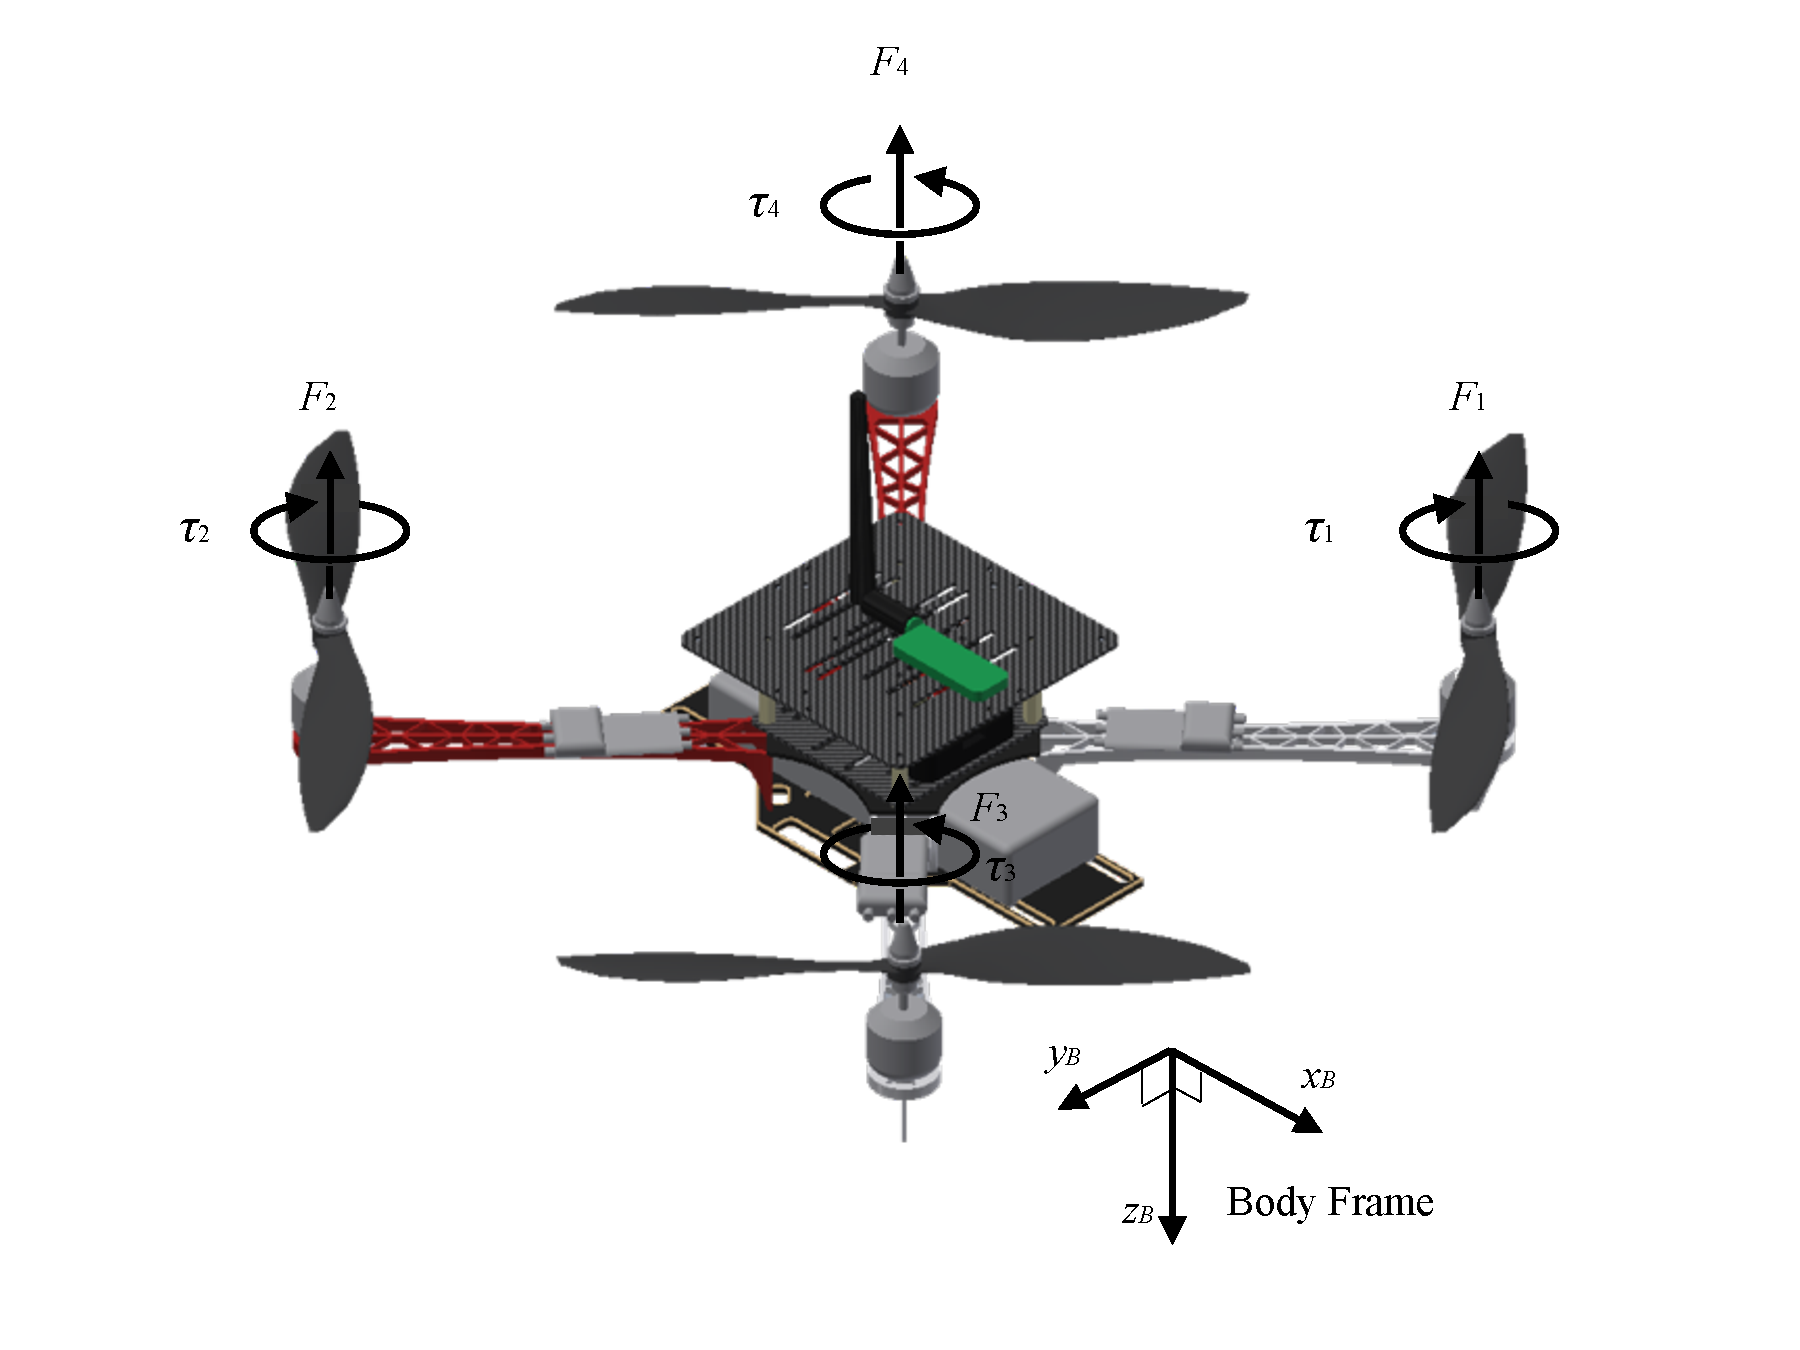
\includegraphics[width=0.8\textwidth]{graphics/mixer.pdf}
    \caption{Thrust and Torque Generated by Each Rotor}
    \label{fig:mixer}
\end{figure}

In the mixer, the magnitude of the desired thrust \(F_d\) from the outer-loop and the desired attitude control \({\boldsymbol \tau} = (\tau_{\phi}, \tau_{\theta}, \tau_{\psi})\) from the inner-loop are received. In order to map the attitude control and the desired thrust into motor speed \( {\boldsymbol n} = (n_1, n_2, n_3, n_4)\) , an aerodynamic model of the quadrotor can be applied.

It is known that the property of propeller is given with non-dimensional thrust coefficient \(C_T\) and power coefficient \(C_P\) as, \\
\begin{equation}
\begin{aligned}
C_T (n_i) ={ T \over { \rho {n_i}^2 D^4}}
\end{aligned}
\end{equation}
\begin{equation}
\begin{aligned}
C_P (n_i) = {P \over { \rho {n_i}^3 D^5}}
\end{aligned}
\end{equation}
where \(\rho\) is the density of air, \(D\) is the propeller's diameter, and \(T\), \(P\) are thrust and torque generated by a propeller, respectively \cite{airfoil2}. Here, \(C_T\) and \(C_P\) change according to rotation speed, and their curves are varied across different geometry of propellers and other conditions. Let \(F_i \) be the thrust force of each motor (\( i = 1, 2, 3, 4 \)) corresponding to its motor speed \( n_i\). With the experimental data of \(C_T\) and \(C_P\), thrust \( F_i\) and torque \(\tau_i\) generated by a motor according to its motor speed \( n_i\) are given as below,\\
\begin{equation}
\begin{aligned}
F_i = C_T (n_i) \rho {n_i}^2 D^4
\end{aligned}
\end{equation}
\begin{equation}
\begin{aligned}
\tau_i & = {P \over {2 \pi n_i}} \\ 
& = {C_P (n_i) \rho {n_i}^2 D^5 \over {2 \pi}}
\end{aligned}
\end{equation}

Since the quadrotor uses an X-shape frame in which the formation of the motors is a square, there is a linear relation as, \\
\begin{equation}
\begin{aligned}
F & = F_1 + F_2 + F_3 + F_4 \\
\tau_{\phi} & = {l \over {\sqrt{2}}} ( - F_1 + F_2 + F_3 - F_4)\\
\tau_{\theta} & = { l \over {\sqrt{2}}} (  F_1 - F_2 + F_3 - F_4)\\
\tau_{\psi} & =  \tau_1 + \tau_2 - \tau_3 - \tau_4
\end{aligned}
\end{equation}
where \(l\) to the length of the frame \cite{randal08}. We define an aerodynamic coefficient matrix \(B ({\boldsymbol n})\) as,
\begin{equation}
\begin{aligned}
B ({\boldsymbol n}) = 
\begin{bmatrix}
C_T (n_1)	& C_T (n_2)	& C_T (n_3)	& C_T (n_4)\\
- {l \over{\sqrt{2}}} C_T (n_1)		& {l \over{\sqrt{2}}} C_T (n_2)		& {l \over{\sqrt{2}}} C_T (n_3)	& - {l \over{\sqrt{2}}} C_T (n_4) \\
{l \over{\sqrt{2}}} C_T (n_1)		& - {l \over{\sqrt{2}}} C_T (n_2)		& {l \over{\sqrt{2}}} C_T (n_3)	& - {l \over{\sqrt{2}}} C_T (n_4) \\
{D \over{2\pi}} C_P (n_1)			& {D \over{2\pi}} C_P	 (n_2)		& - {D \over{2\pi}} C_P (n_3)	& - {D \over{2\pi}} C_P (n_4)
\end{bmatrix}
\end{aligned}
\end{equation}
Then, the above equation can be written as,\\
\begin{equation}
\label{eq:u_n}
\begin{aligned}
\begin{bmatrix}
F_d\\
u_p\\
u_q\\
u_r
\end{bmatrix}
= \rho D^4 B ({\boldsymbol n})
\begin{bmatrix}
{n_1}^2 \\
{n_2}^2 \\
{n_3}^2 \\
{n_4}^2
\end{bmatrix}
\end{aligned}
\end{equation}
With the above equation, motor speed \({\boldsymbol n} \) corresponding to the magnitude of the desired thrust \(F_d\) and the attitude control \({\boldsymbol \tau}\) can be computed as, \\
\begin{equation}
\label{eq:n_u}
\begin{aligned}
\begin{bmatrix}
{n_1}^2 \\
{n_2}^2 \\
{n_3}^2 \\
{n_4}^2
\end{bmatrix}
= {1 \over \rho D^4 }B^{-1} ({\boldsymbol n})
\begin{bmatrix}
F_d\\
u_p\\
u_q\\
u_r
\end{bmatrix}
\end{aligned}
\end{equation}


%%%%%%%%%%%%%%%%%%%%%%%%%%%%%%%%%%%%%%%%%%%%%%%%%%%%%%%%%%%%%%%%%%%%%%%%%%%%%%%%%%%%%%%%%%%%%%
\subsection{Approximation of the Aerodynamic Coefficient Matrix}
Since the coefficient matrix \( B ({\boldsymbol n}) \) is not independent from motor speed \(n_i\), it is difficult to compute a solution of Equation (\ref{eq:n_u}). To solve the problem, the linear approximation in terms of \(1 \over {n_i}^2\) as,\\
\begin{equation}
\label{eq:ct_approx}
\begin{aligned}
C_T ({n_i}) & = {C_T}_0 + {C_T}_1 {1 \over {n_i}^2} + O \left({1 \over {n_i}^4} \right) \\
& \approx {C_T}_0 + {C_T}_1 {1 \over {n_i}^2} \\
\end{aligned}
\end{equation}
\begin{equation}
\label{eq:cp_approx}
\begin{aligned}
C_P ({n_i}) & = {C_P}_0 + {C_P}_1 {1 \over {n_i}^2} + O \left({1 \over {n_i}^4} \right) \\
& \approx {C_P}_0 + {C_P}_1 {1 \over {n_i}^2}
\end{aligned}
\end{equation}
can be applied. Then, Equation (\ref{eq:u_n}) can be written as, \\
\begin{equation}
\begin{aligned}
\begin{bmatrix}
F_d\\
u_p\\
u_q\\
u_r
\end{bmatrix}
\approx \rho D^4 \left( B_0
\begin{bmatrix}
{n_1}^2 \\
{n_2}^2 \\
{n_3}^2 \\
{n_4}^2
\end{bmatrix}
+ B_1 
\begin{bmatrix}
1\\
1\\
1\\
1
\end{bmatrix} \right)
\end{aligned}
\end{equation}
where the approximation terms of \( B_0\), \(B_1\) of the matrix \(B ({\boldsymbol n}) \) are defined as,
\begin{equation}
\begin{aligned}
B_0 = 
\begin{bmatrix}
{C_T}_0	& {C_T}_0 	& {C_T}_0		& {C_T}_0 \\
- {l \over{\sqrt{2}}} {C_T}_0		& {l \over{\sqrt{2}}} {C_T}_0		& {l \over{\sqrt{2}}} {C_T}_0	& - {l \over{\sqrt{2}}} {C_T}_0 \\
{l \over{\sqrt{2}}} {C_T}_0		& - {l \over{\sqrt{2}}} {C_T}_0		& {l \over{\sqrt{2}}} {C_T}_0	& - {l \over{\sqrt{2}}} {C_T}_0 \\
{D \over{2\pi}} {C_P}_0			& {D \over{2\pi}} {C_P}_0		& - {D \over{2\pi}} {C_P}_0		& - {D \over{2\pi}} {C_P}_0
\end{bmatrix}
\end{aligned}
\end{equation}
\begin{equation}
\begin{aligned}
B_1 = 
\begin{bmatrix}
{C_T}_1	& {C_T}_1 	& {C_T}_1		& {C_T}_1 \\
- {l \over{\sqrt{2}}} {C_T}_1		& {l \over{\sqrt{2}}} {C_T}_1		& {l \over{\sqrt{2}}} {C_T}_1	& - {l \over{\sqrt{2}}} {C_T}_1 \\
{l \over{\sqrt{2}}} {C_T}_1		& - {l \over{\sqrt{2}}} {C_T}_1		& {l \over{\sqrt{2}}} {C_T}_1	& - {l \over{\sqrt{2}}} {C_T}_1 \\
{D \over{2\pi}} {C_P}_1			& {D \over{2\pi}} {C_P}_1		& - {D \over{2\pi}} {C_P}_1	& - {D \over{2\pi}} {C_P}_1
\end{bmatrix}
\end{aligned}
\end{equation}
Then, desired motor speeds \( \boldsymbol n\) are easily computed from the below equation,
\begin{equation}
\begin{aligned}
\begin{bmatrix}
{n_1}^2 \\
{n_2}^2 \\
{n_3}^2 \\
{n_4}^2
\end{bmatrix}
\approx
{B_0}^{-1}
\left(
{1 \over {\rho D^4}}
\begin{bmatrix}
F_d\\
u_p\\
u_q\\
u_r
\end{bmatrix}
- B_1
\begin{bmatrix}
1\\
1\\
1\\
1
\end{bmatrix}
\right)
\end{aligned}
\end{equation}

\begin{figure}
    \centering
    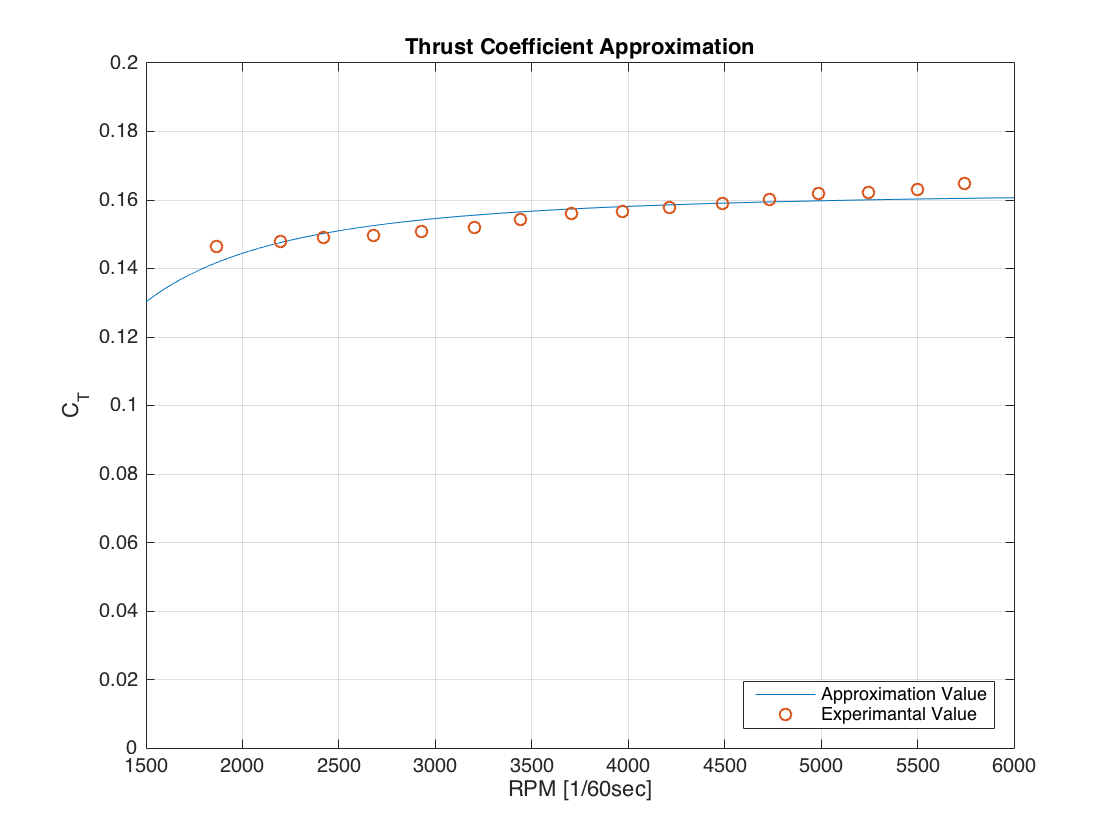
\includegraphics[width=0.8\textwidth]{graphics/Ct_fig.png}
    \caption{Comparison of experimental and approximated thrust coefficient}
    \label{fig:ct}
    
    \vspace{1cm}
    
    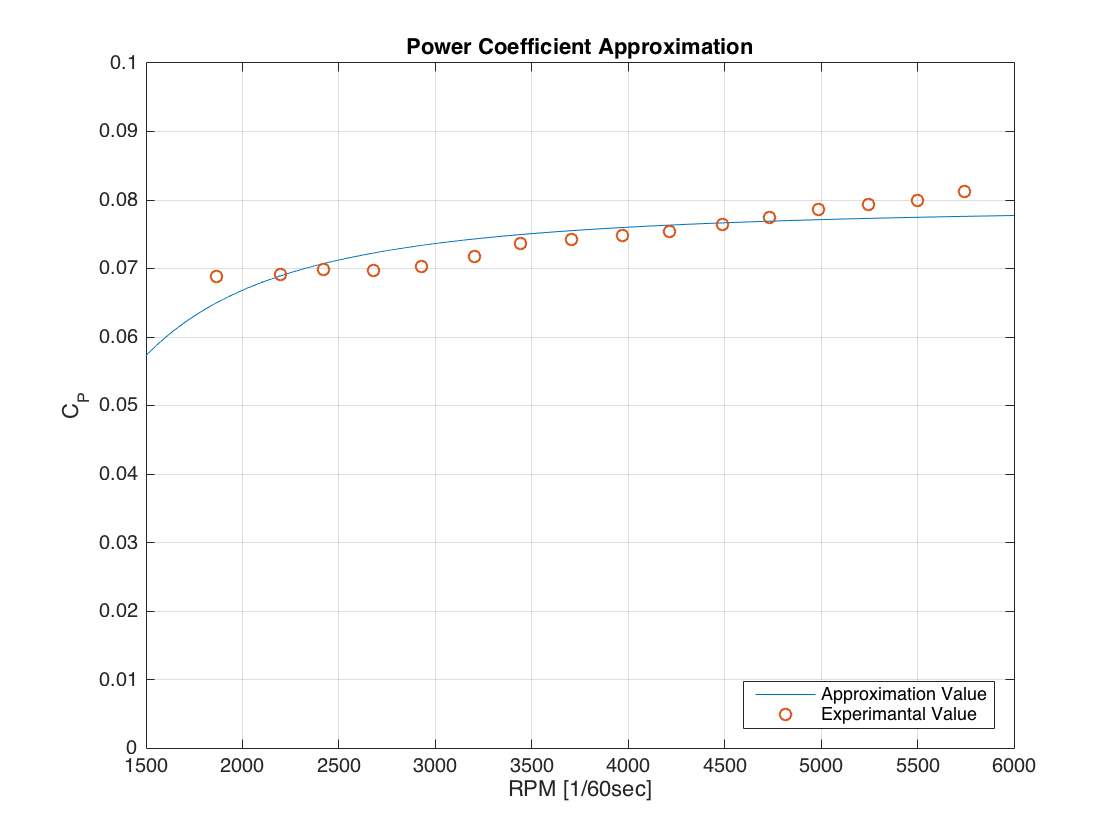
\includegraphics[width=0.8\textwidth]{graphics/Cp_fig.png}
    \caption{Comparison of experimental and approximated power coefficient}
    \label{fig:cp}
\end{figure}

To compute the model of thrust coefficient (\ref{eq:ct_approx}) and power coefficient (\ref{eq:cp_approx}), the experimental data of the propeller APC 10 \(\times\) 4.7 in the UIUC Propeller Database Vol.1 are used, and the method of least mean square error (LMSE) linear regression is applied in terms of \(1 \over {{n_i}^2}\) \cite{airfoil}. The approximated models of \(C_T (n_i)\) and \(C_P (n_i)\) are given as Equations (\ref{eq:ct}) and (\ref{eq:cp}), and the experimental data and the approximated models are compared in the Figures \ref{fig:ct}, \ref{fig:cp}. \\
\begin{equation}
\label{eq:ct}
\begin{aligned}
C_T ({n_i}) & = 0.1627 -73047 \times {1 \over {n_i}^2} \\
\end{aligned}
\end{equation}
\begin{equation}
\label{eq:cp}
\begin{aligned}
C_P ({n_i}) & = 0.0791 - 49112 \times {1 \over {n_i}^2} \\
\end{aligned}
\end{equation}
%%%%%%%%%%%%%%%%%%%%%%%%%%%%%%%%%%%%%%%%%%%%%%%%%%%%%%%%%%%%%%%%%%%%%%%%%%%%%%%%%%%%%%%%%%%%%%
\subsection{Motor Control}
In the quadrotor system, propellers are rotated by four brushless DC motors. In order to control DC motors, the method of pulse width modulation (PWM) is often used. In the PWM method, an average of constant-voltage pulsing signals actuates a motor \cite{audio}. Therefore, motor voltage is controllable by changing a pulse signal's width. Let \(d_{pwm}\) be duty cycle as, \\
\begin{equation}
\begin{aligned}
d_{pwm} = H f_{pwm} : \quad 0 \le d_{pwm} \le 1
\end{aligned}
\end{equation}
where \(H\) is signal width and \(f_{pwm}\) is the fixed frequency of signals. Then, the relation between motor voltage \(V_{mot}\) and duty cycle \(pwm\) is formalized as, \\
\begin{equation}
\label{eq:pwm_voltage}
\begin{aligned}
V_{mot} = d_{pwm} V_0
\end{aligned}
\end{equation}
where \(V_0\) is the constant voltage of signals.

The electric and dynamic models of a DC motor are given in terms of motor speed \(n\) and \(V_{mot}\) as,
\begin{equation}
\label{eq:motor_dynamics_01}
\begin{aligned}
V_{mot} & = 2 \pi k_{b} n + R i + L {{di}\over {dt}}\\
\end{aligned}
\end{equation}
\begin{equation}
\label{eq:motor_dynamics_02}
\begin{aligned}
k_m i & = 2 \pi k_f n + 2 \pi I_{mot} {{dn} \over {dt} } + M_R \text{sgn} (n)
\end{aligned}
\end{equation}
where \(k_{b} \), \(k_f\), \(k_m\) are the motor's torque constant, back electromotive force constant, and viscous damping coefficient, respectively. \(M_R\) is frictional torque, \(R\) is the motor's internal resistor, and \(L\) is the motor's internal inductance \cite{Mahfouz13}. \(I_{mot}\) is the total inertia of the motor and the propeller. Then, the above equation is written as the following second-order system with respect to motor speed \(n\). \\
\begin{equation}
\label{eq:motor_model_01}
\begin{aligned}
V_{mot} = 2 \pi \left( (k_b + {{R k_f}\over{k_m}} ) n + {1 \over {k_m}}( {R I_{mot}} + L k_f ) {{dn}\over{dt}} + {{L I_{mot}} \over {k_m} } {{d^2 n}\over{{dt}^2}}  \right) + R M_R \text{sgn} (n) : \quad n \neq 0\\
\end{aligned}
\end{equation}
Also, from Equation (\ref{eq:motor_dynamics_02}), there is a voltage threshold due to frictional torque so that a motor doesn't spin below the threshold. \\

Assuming motor speed changes smoothly so that the effect of internal resistor and inductance is small enough, Equation (\ref{eq:motor_model_01}) can be simplified as, \\
\begin{equation}
\label{eq:motor_model_02}
\begin{aligned}
V_{mot} \approx 2 \pi  (k_b + {{R k_f}\over{k_m}} ) n  + R M_R \text{sgn} (n)
\end{aligned}
\end{equation}
Define composite coefficients of the tangent \(\alpha\), and the intercept \(\beta\) as, 
\begin{equation}
\begin{aligned}
\alpha = {{k_m V_0} \over {2 \pi (k_b k_m + R k_f )}} 
\end{aligned}
\end{equation}
\begin{equation}
\begin{aligned}
\beta = {{k_m R M_R} \over {2 \pi (k_b k_m + R k_f )}} 
\end{aligned}
\end{equation}
Then, from Equations (\ref{eq:pwm_voltage}) and (\ref{eq:motor_model_02}), the relation between the motor speed \(n\) and the duty cycle \(d_{pwm}\) is written as the below equation.  \\
\begin{equation}
\label{eq:motor_curve_01}
\begin{aligned}
n \approx 
\begin{cases}
     \alpha d_{pwm}  - \beta \quad &  d_{threshold} \le d_{pwm} \le 1 \\
    0  \quad &   d_{pwm} \le  d_{threshold} \\
  \end{cases}
  \end{aligned}
\end{equation}

\begin{figure}
    \centering
    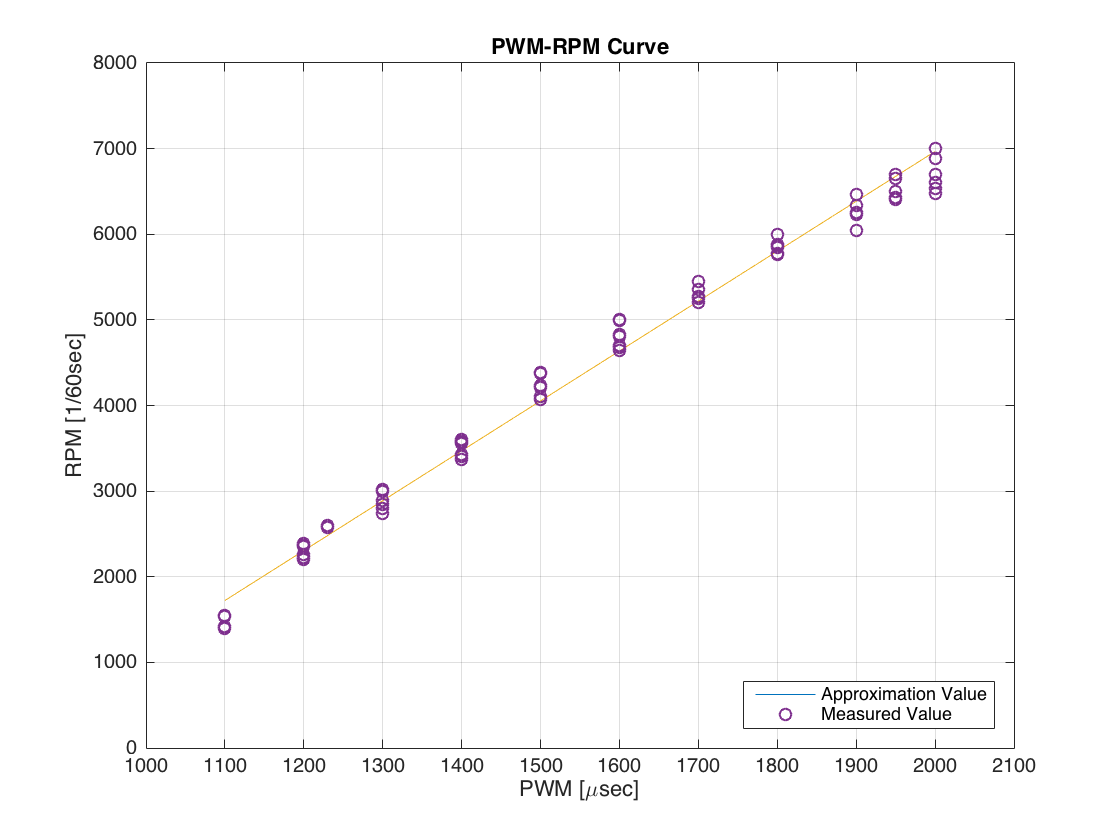
\includegraphics[width=0.8\textwidth]{graphics/pwm_rpm_curve.png}
    \caption{Change of RPM output corresponding to PWM command}
    \label{fig:pwm_rpm}
\end{figure}
If the characteristic information of the motors is available, the parameters \(\alpha\), \(\beta\) of the model of Equation (\ref{eq:motor_curve_01}) can be computed. However, there is no available information about the motor constants, it is necessary to calibrate the relation between PWM input and RPM output of a motor with a propeller. Therefore, the composite parameters of the gradient \(\alpha\) and the intercept \(\beta\) are calibrated by experiments. In the calibration, a reflective marker sticker is put on each propeller, and a tachometer measures rotation speed of the markers. PWM signal of voltage is controlled by an ESC, and the range of PWM command is set to be between 1000 \(\mu\)sec and 2000 \(\mu\)sec. The result of the experiment and the approximated model by the LMSE linear regression method are shown in Figure \ref{fig:pwm_rpm} and Equation (\ref{eq:motor_curve_02}).\\
\begin{equation}
\label{eq:motor_curve_02}
\begin{aligned}
n = 
\begin{cases}
     0.1716 \times d_{pwm}  - 803.4 \quad &  1100 \le d_{pwm} \le 2000 \\
    0  \quad &   \text{otherwise} \\
  \end{cases}
  \end{aligned}
\end{equation}


Since a brushless DC motor used in the quadrotor system does not have an encoder to measure its motor speed, open-loop control based on Equation (\ref{eq:motor_curve_02}) is applied to control motor speed. Also, PWM command is limited to be between 1230 \(\mu\)sec and 1950 \(\mu\)sec to prevent inappropriate performance.


\chapter{Evaluation of the Control System}
\label{ch:evaluation}

In this chapter, in order to validate the advantage of the control system stated in Chapter \ref{ch:control_system}, the nonlinear attitude control and an conventional PID attitude control are compared with each other, by simulation and flight experiments. First, the PID attitude control used for comparison and its linear mapping model are described. Then, the simulation setup is explained, and the simulation results of the two control systems are presented. Finally, the experimental setup is described, and the trajectory results of the two control systems are analyzed and discussed.

\section{Linear Attitude Control for Comparison}
\label{sec:pid}

To compare with the nonlinear control system of Chapter \ref{ch:control_system}, a conventional inner-loop controller is also tested for comparison. In the linear controller, derivative of desired attitude \( \dot{ {\boldsymbol \eta}_d } \) is also computed as described in Subsection \ref{subsec:desired_attitude}. Similarly, the reference angular velocity \({\boldsymbol \omega}_r = (p_r, q_r, r_r)\) is given as the below equation.\\
\begin{equation}
\begin{aligned}
{\boldsymbol \omega}_r & = Z^{-1} \dot{\boldsymbol \eta}_r \\
&  = Z^{-1} \dot{ {\boldsymbol \eta}_d } +  Z^{-1} \Lambda ({\boldsymbol \eta}_d - {\boldsymbol \eta})\\
\end{aligned}
\end{equation}

However, instead of Equation (\ref{eq:control_law}) of the nonlinear control system, PID control with respect to the quadrotor's angular velocity is applied to the linear controller. For convenience, we assumed that the derivative of the reference angular velocity is zero. The control law is given as,\\
\begin{equation}
\begin{aligned}
{u_p} & = {{k_P}_{\phi}}(p_r - {p}) + {{k_D}_{\phi}}{\dot {p}} + {{k_I}_{\phi}} \int_{t_0}^{t} {(p_r - {p})} dt\\
{u_q} & = {{k_P}_{\theta}}(q_r - {q}) + {{k_D}_{\theta}}{\dot {q}} + {{k_I}_{\theta}} \int_{t_0}^{t} {(q_r - {q})} dt\\
{u_r} & = {{k_P}_{\psi}}(r_r - {r}) + {{k_D}_{\psi}}{\dot {r}} + {{k_I}_{\psi}} \int_{t_0}^{t} {(r_r - {r})} dt\\
\end{aligned}
\end{equation}
Also, the mixer uses more simplified linear model as below, instead of Equation (\ref{eq:n_u}). The matrix for mapping the desired torques into desired motor speed is constant as the below equations.
\begin{equation}
\begin{aligned}
\begin{bmatrix}
n_1\\
n_2\\
n_3\\
n_4
\end{bmatrix}
= M^{-1}
\begin{bmatrix}
k_f F_d\\
u_p\\
u_q\\
u_r
\end{bmatrix}
\end{aligned}
\end{equation}
where \(k_f\) is a gain for the scale of thrust, and \(M\) is defined as, \\
\begin{equation}
\begin{aligned}
M = 
\begin{bmatrix}
1 				& 1				& 1				& 1 \\
- {1\over{\sqrt{2}}}	&   {1\over{\sqrt{2}}}	& {1\over{\sqrt{2}}}	& - {1\over{\sqrt{2}}} \\
  {1\over{\sqrt{2}}}	& - {1\over{\sqrt{2}}}	& {1\over{\sqrt{2}}}	& - {1\over{\sqrt{2}}} \\
1				& 1				& - 1				& -1\\
\end{bmatrix}
\end{aligned}
\end{equation}
The matrix \(M\) represents only the proportional effect of each motor on torques and thrusts due to the geometry of the frame. Other physical factors, such as motor dynamics, are ignored as tuning the gains of the attitude PID control.


\section{Simulation Study for Inner-loop Controller}
\label{sec:simulation}

It is difficult to evaluate the performance of the control systems in a limited area since changing and holding the quadrotor's attitude makes the quadrotor to move out of our physical test area. Therefore, it is more suitable to use simulation rather than real flight for evaluation of the quadrotor's performance.

The PID inner-loop controller and a linear mapping model from torque into motor speeds described in Section \ref{sec:pid} are often used for attitude control of a quadrotor. Let it be called "linear attitude controller". In this section, simulations of the linear and nonlinear attitude control systems are stated, and comparison of the results is discussed to validate the advantage of the control system stated in Chapter \ref{ch:control_system}. First, setup for simulation is explained., and then, simulation results of the two control systems are discussed.

%%%%%%%%%%%%%%%%%%%%%%%%%%%%%%%%%%%%%%%%%%%%%%%%%%%%%%%%%%%%%%%%%%%%%%%%%%%%%%%%%%%%%%%
\subsection{Simulation Setup}

In simulation, the dynamic models of Equations (\ref{eq:newton_gravity}) and (\ref{eq:rotation}) are applied. The physical quantities of the quadrotor are the same as stated in Chapter \ref{ch:system} in each case. The inner-loop controller was simulated with the following cases; \\
\begin{enumerate}
\item \({\boldsymbol \eta}_d = ({\pi \over{6}}, 0, 0)\)
\item \({\boldsymbol \eta}_d = ({\pi \over{3}}, 0, 0)\)
\item \({\boldsymbol \eta}_d = (0, {\pi \over{6}}, 0)\)
\item \({\boldsymbol \eta}_d = (0, {\pi \over{3}}, 0)\)
\item \({\boldsymbol \eta}_d = (0, 0, {\pi \over{4}})\)
\item \({\boldsymbol \eta}_d = (0, 0, {\pi \over 2})\)
\item \(
\begin{aligned}
{\boldsymbol \eta}_d = 
\begin{cases}
     ({\pi \over{6}}, {\pi \over{6}}, 0) \quad &  1 \le t \le 2 \\
    (-{\pi \over{6}}, -{\pi \over{6}}, 0) \quad & 3 \le t \le 4 \\ 
    (0, 0, 0)  \quad &  \text{otherwise} \\
  \end{cases}
  \end{aligned}
  \)
\end{enumerate}
In every case, the magnitude of thrust control \(F_d\) is constant to be \(mg\), and each controller is well-tuned. 
 
%%%%%%%%%%%%%%%%%%%%%%%%%%%%%%%%%%%%%%%%%%%%%%%%%%%%%%%%%%%%%%%%%%%%%%%%%%%%%%%%%%%%%%%
\subsection{Results}
The results of simulation is shown below. Figure \ref{fig:sim_1} - \ref{fig:sim_7} shows the result of each case in Section \ref{sec:pid}. \\
\begin{figure}[p]
    \centering
    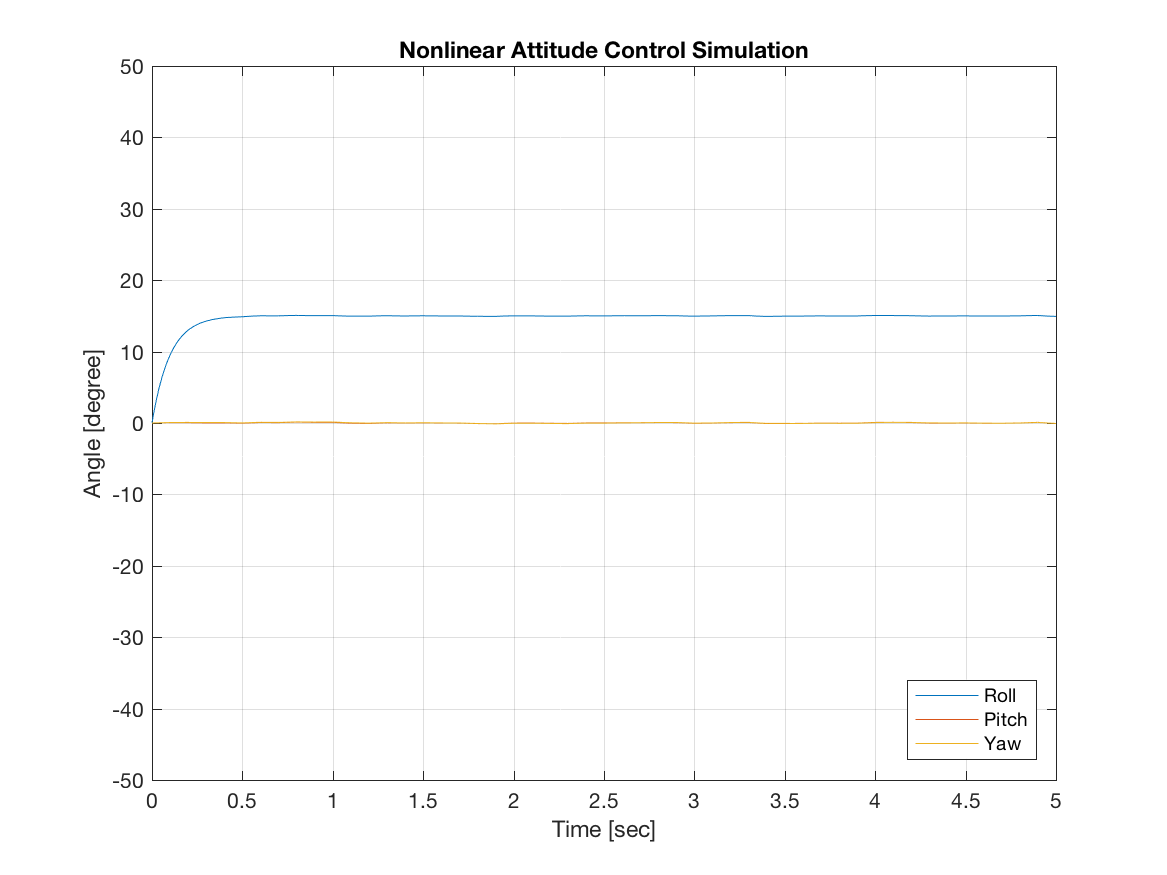
\includegraphics[width=0.45\textwidth]{graphics/phi_03_non.png}
    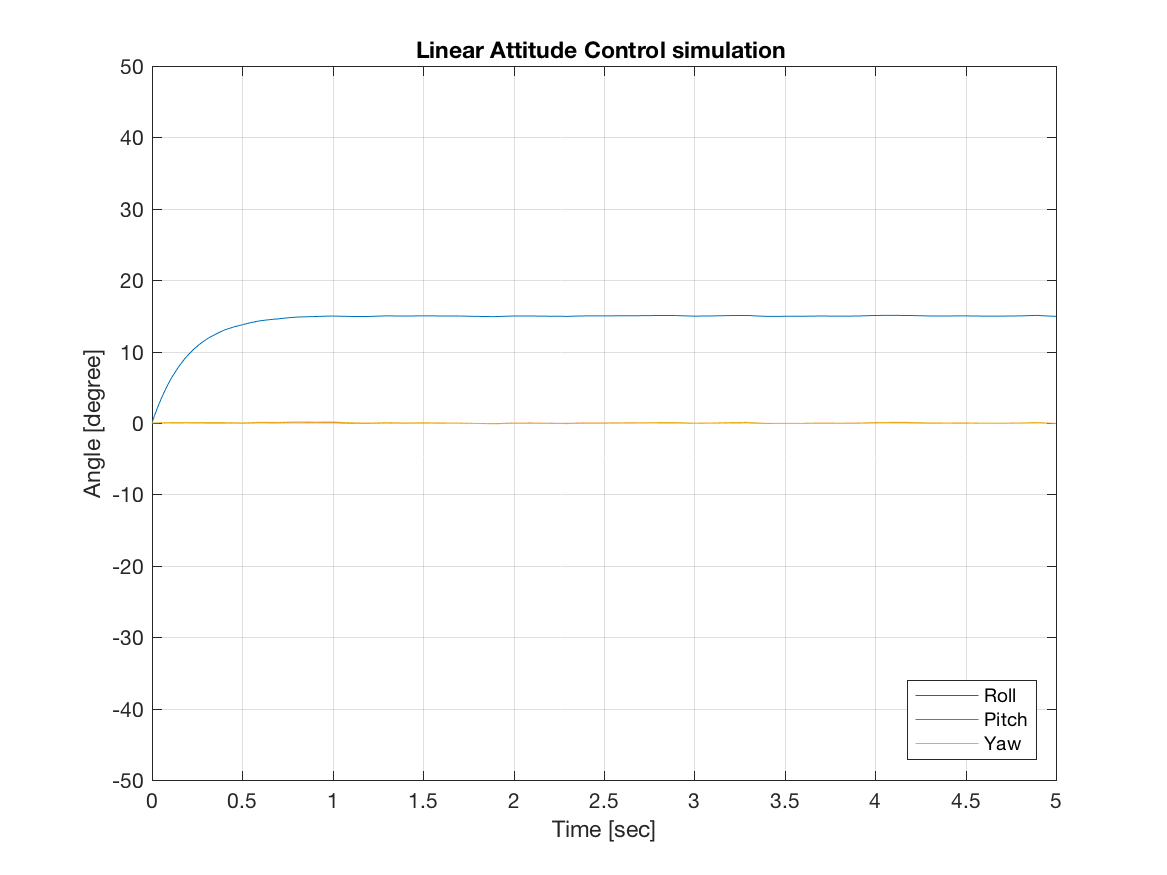
\includegraphics[width=0.45\textwidth]{graphics/phi_03_pid.png}
    \caption{Simulation Result (Case 1)}
    \label{fig:sim_1}
\end{figure}

\begin{figure}
    \centering
    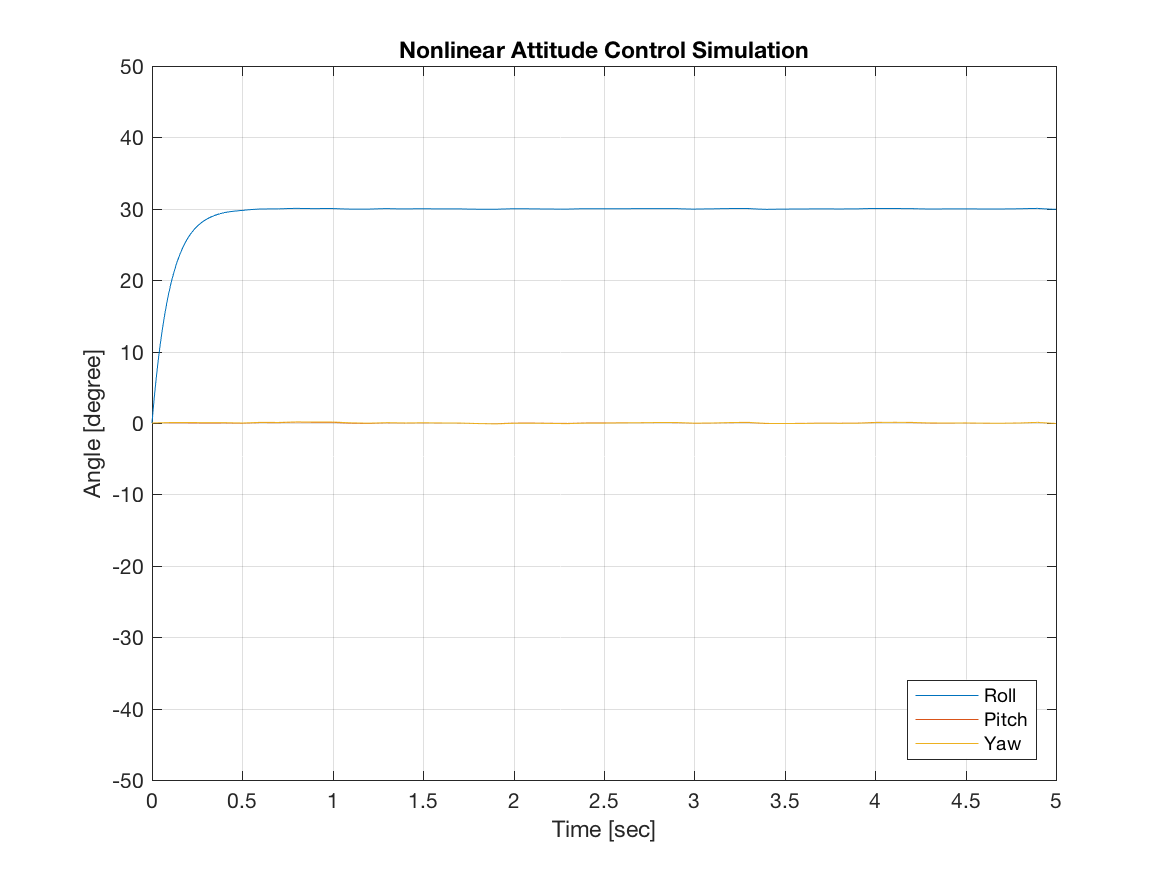
\includegraphics[width=0.45\textwidth]{graphics/phi_05_non.png}
    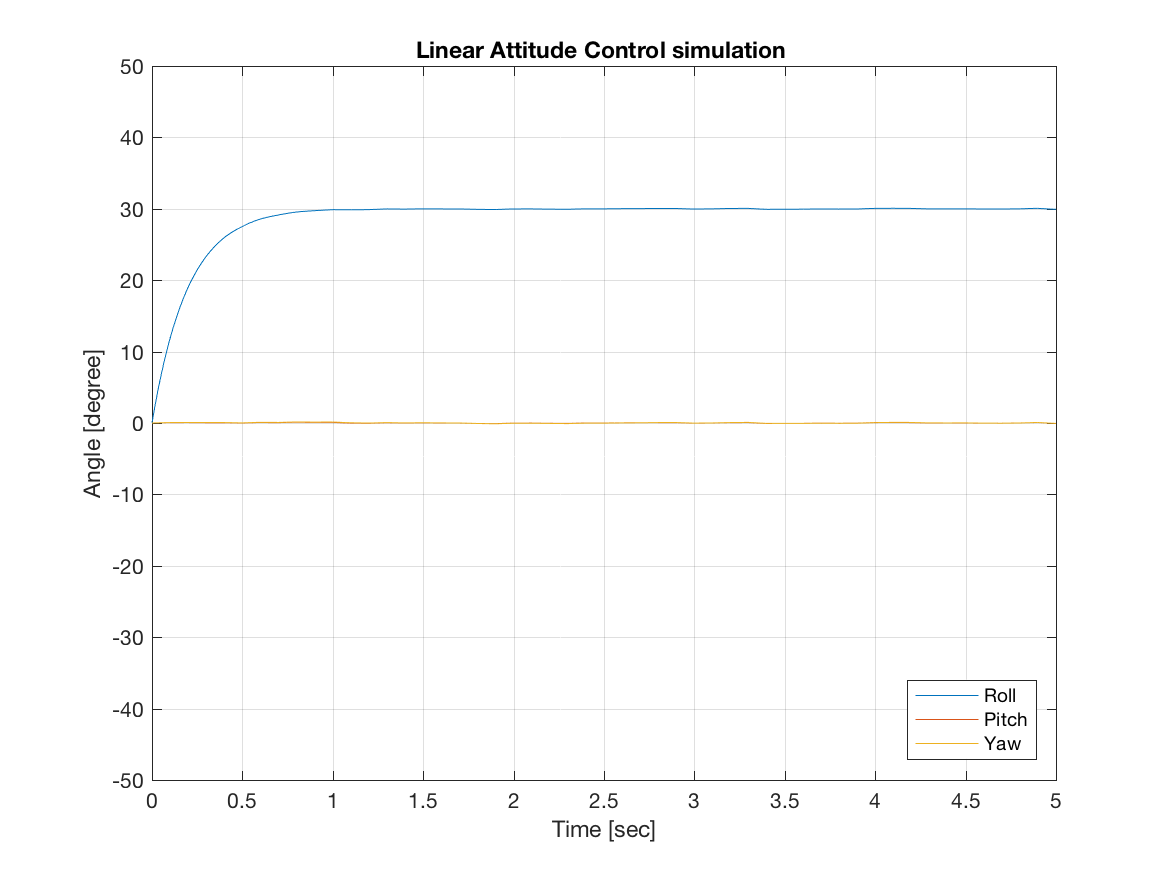
\includegraphics[width=0.45\textwidth]{graphics/phi_05_pid.png}
    \caption{Simulation Result (Case 2)}
    \label{fig:sim_2}
\end{figure}

\begin{figure}
    \centering
    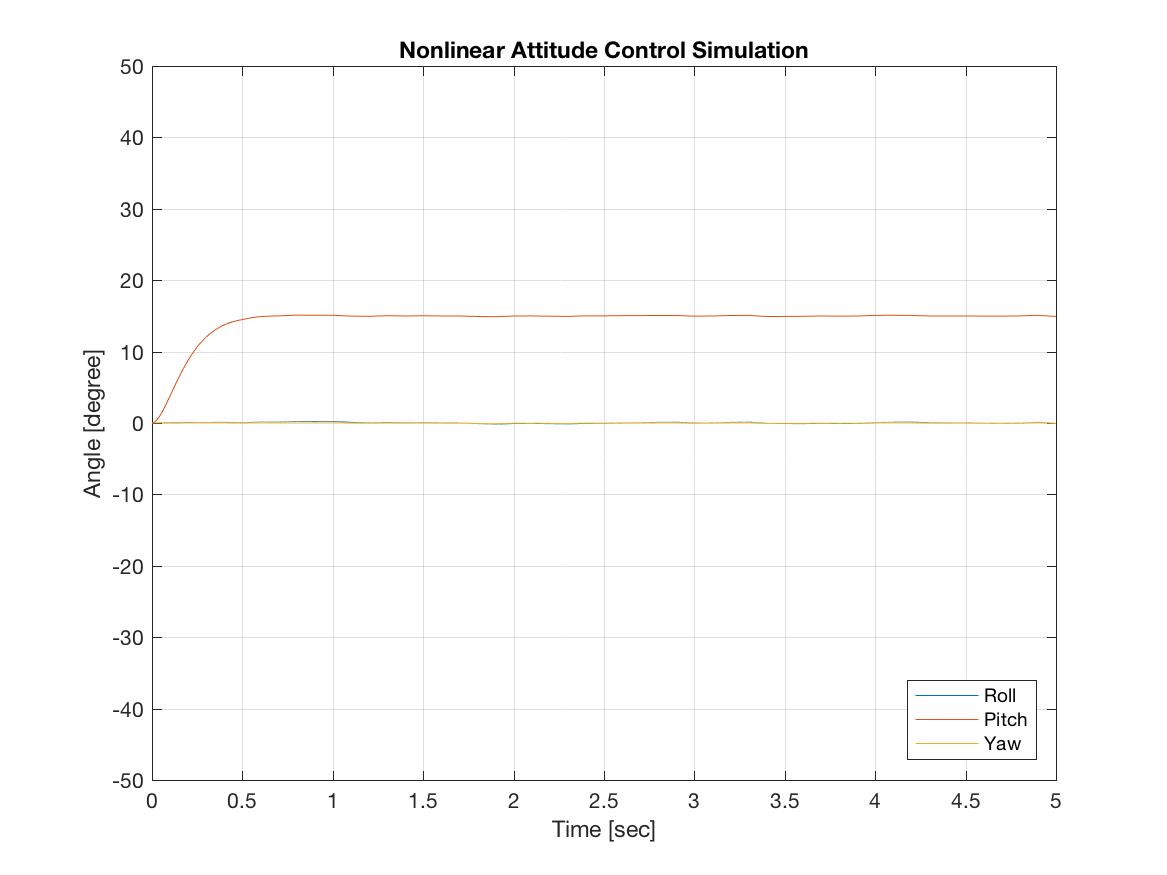
\includegraphics[width=0.45\textwidth]{graphics/theta_03_non.png}
    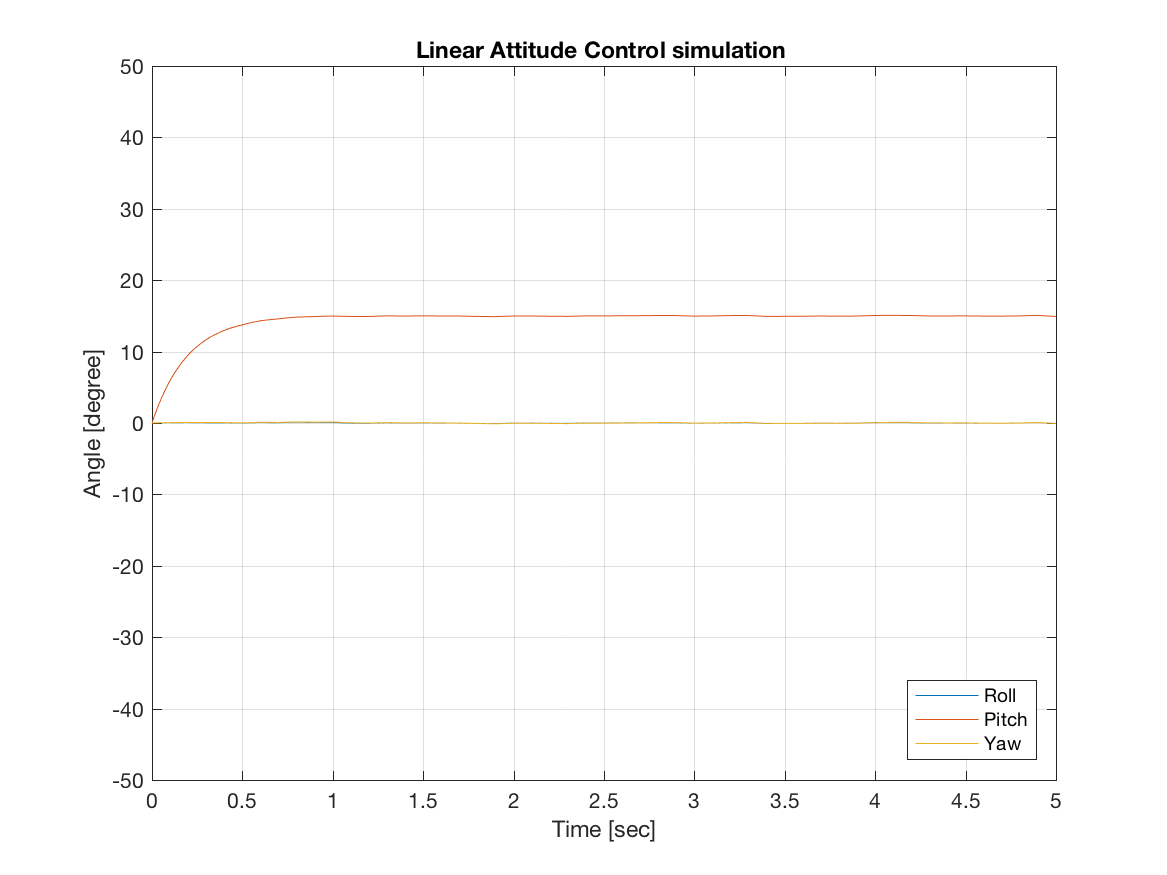
\includegraphics[width=0.45\textwidth]{graphics/theta_03_pid.png}
    \caption{Simulation Result (Case 3)}
    \label{fig:sim_3}
\end{figure}

\begin{figure}
    \centering
    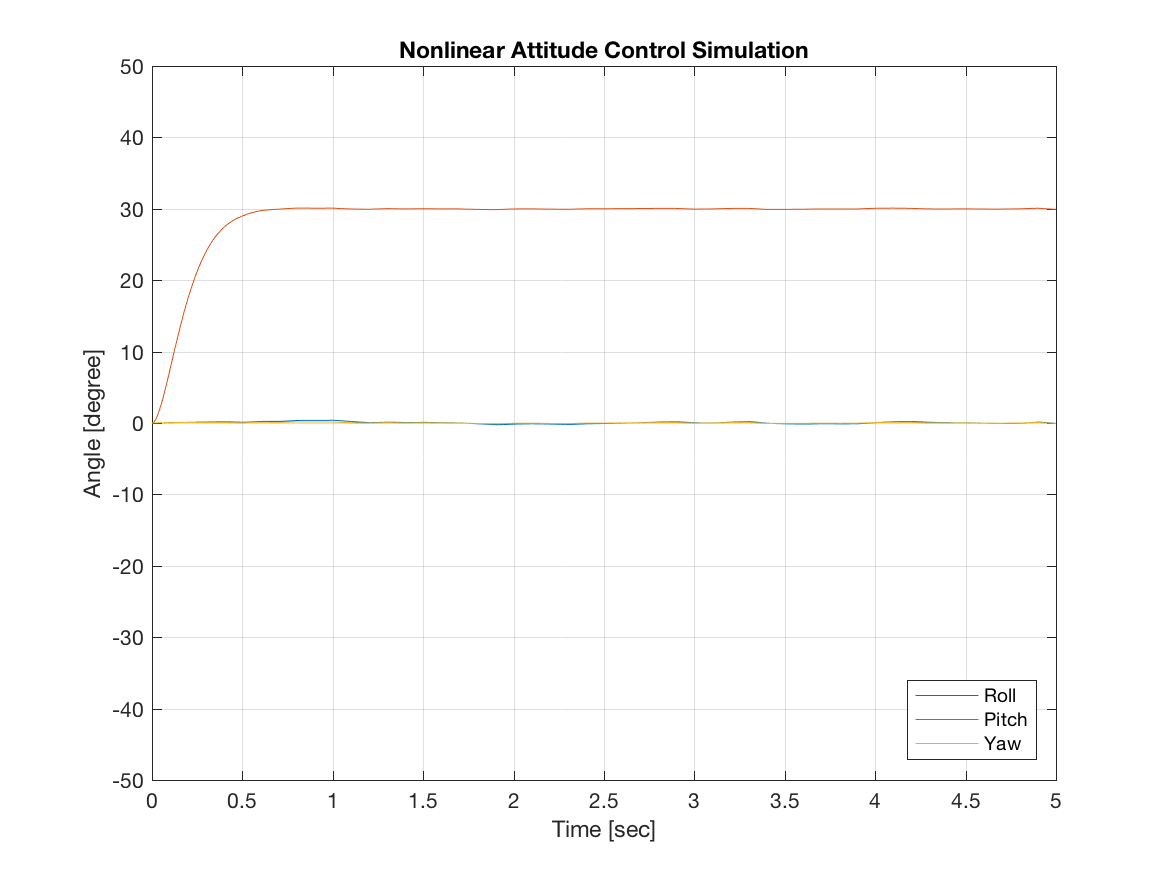
\includegraphics[width=0.45\textwidth]{graphics/theta_05_non.png}
    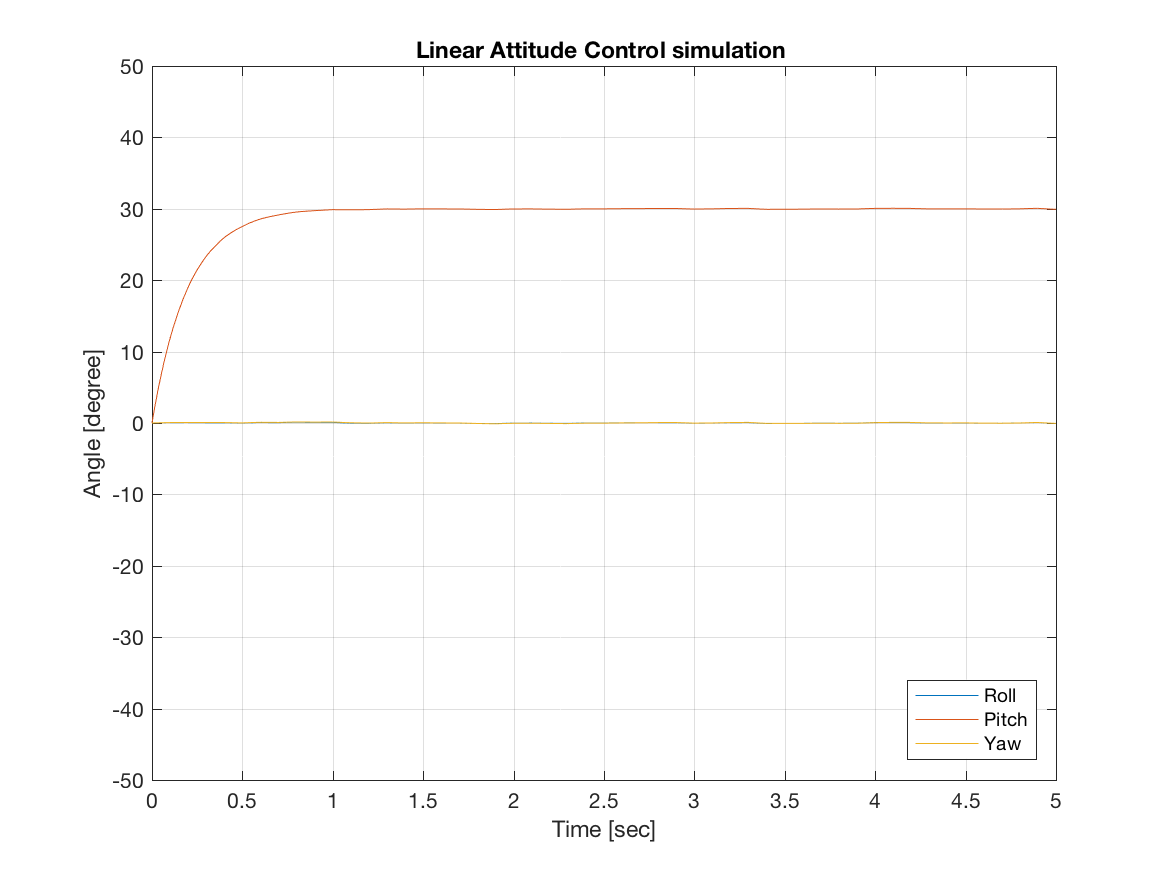
\includegraphics[width=0.45\textwidth]{graphics/theta_05_pid.png}
    \caption{Simulation Result (Case 4)}
    \label{fig:sim_4}
\end{figure}

\begin{figure}
    \centering
    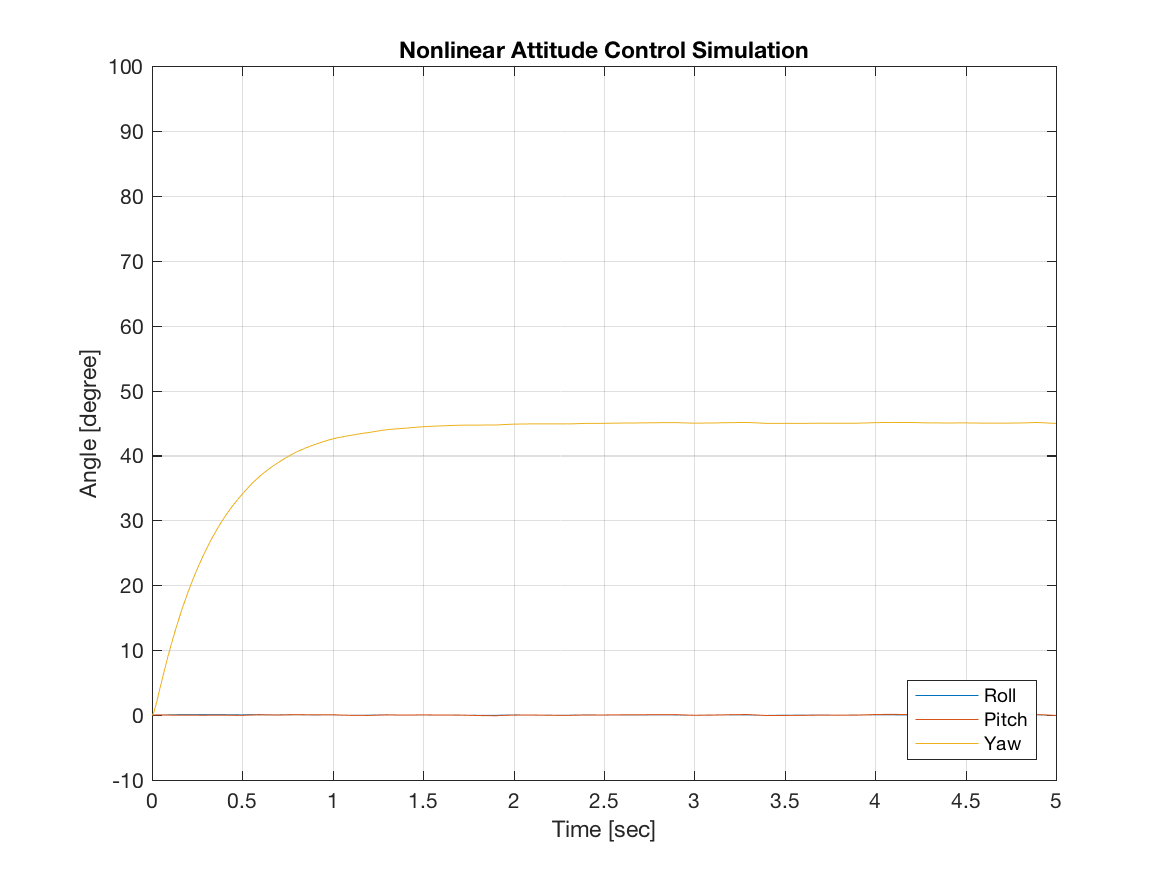
\includegraphics[width=0.45\textwidth]{graphics/yaw_quarter_non.png}
    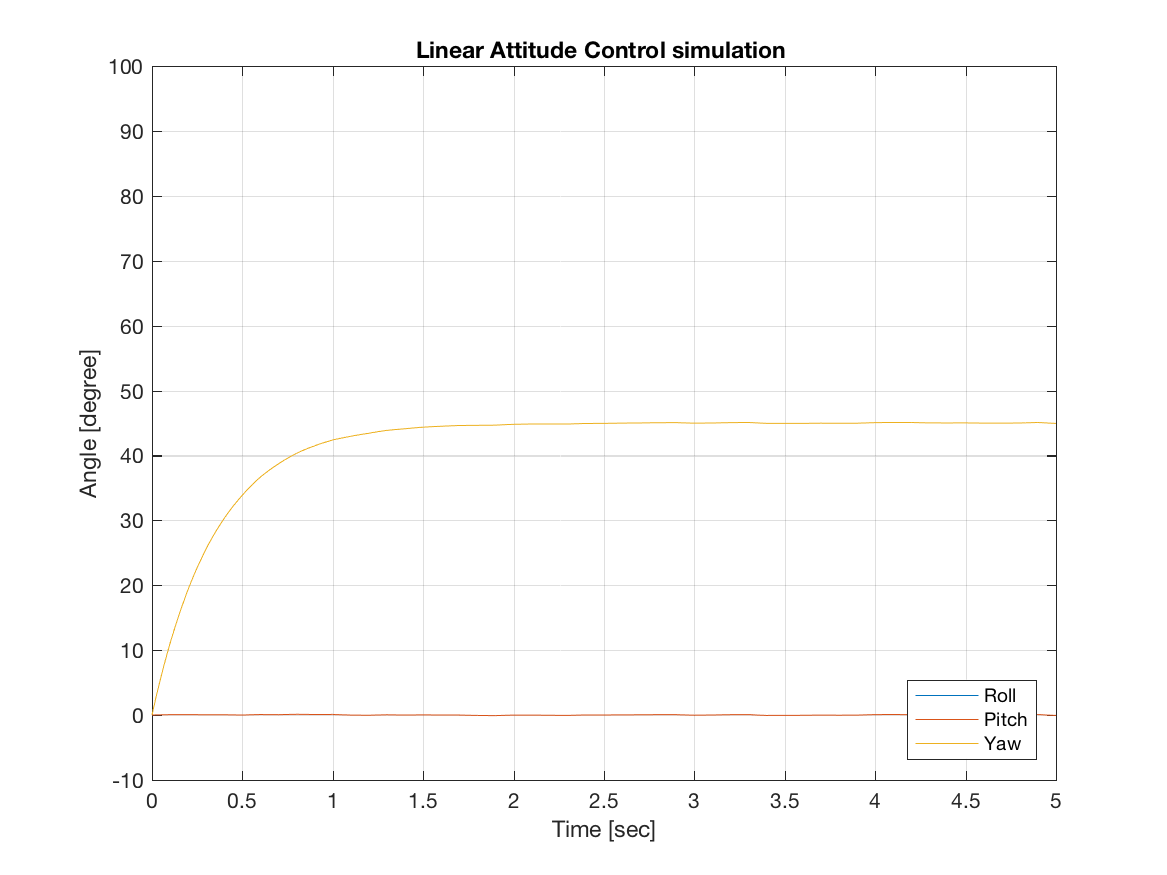
\includegraphics[width=0.45\textwidth]{graphics/yaw_quarter_pid.png}
    \caption{Simulation Result (Case 5)}
    \label{fig:sim_5}
\end{figure}

\begin{figure}
    \centering
    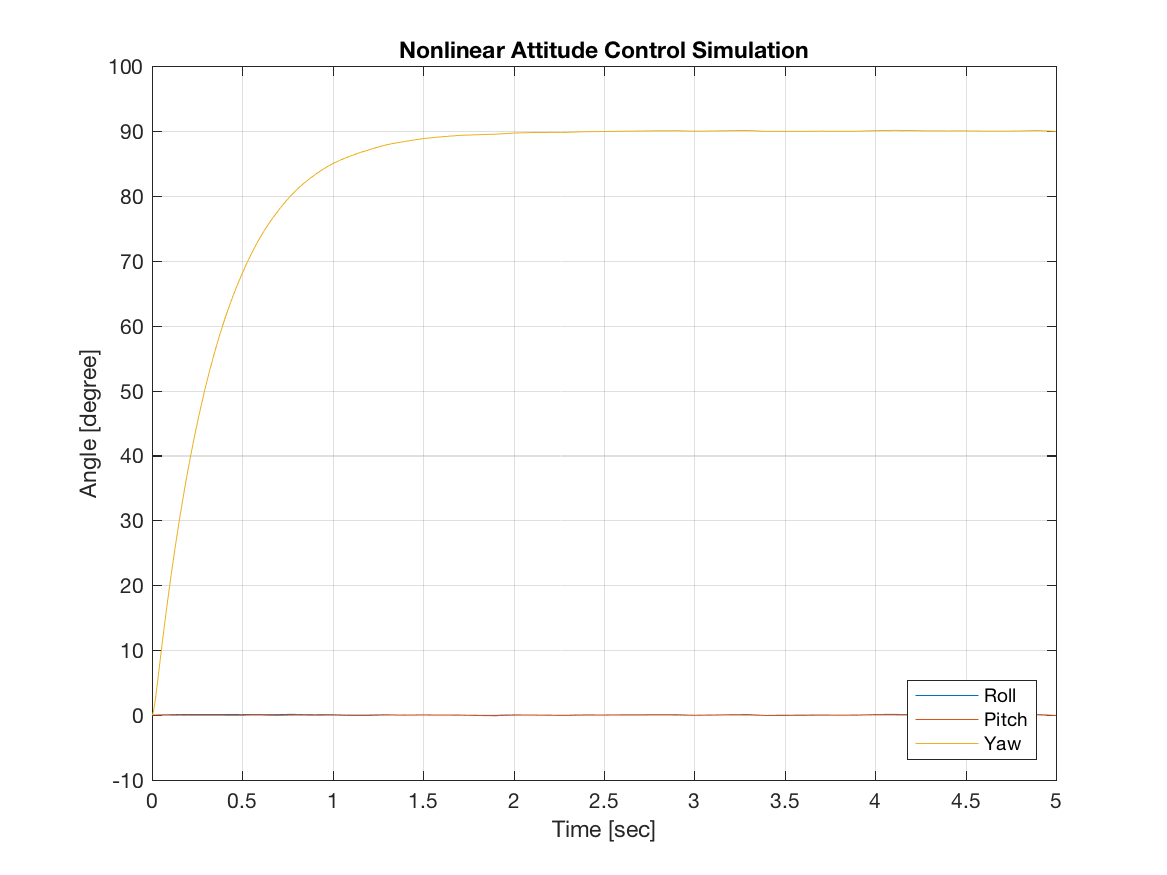
\includegraphics[width=0.45\textwidth]{graphics/yaw_half_non.png}
    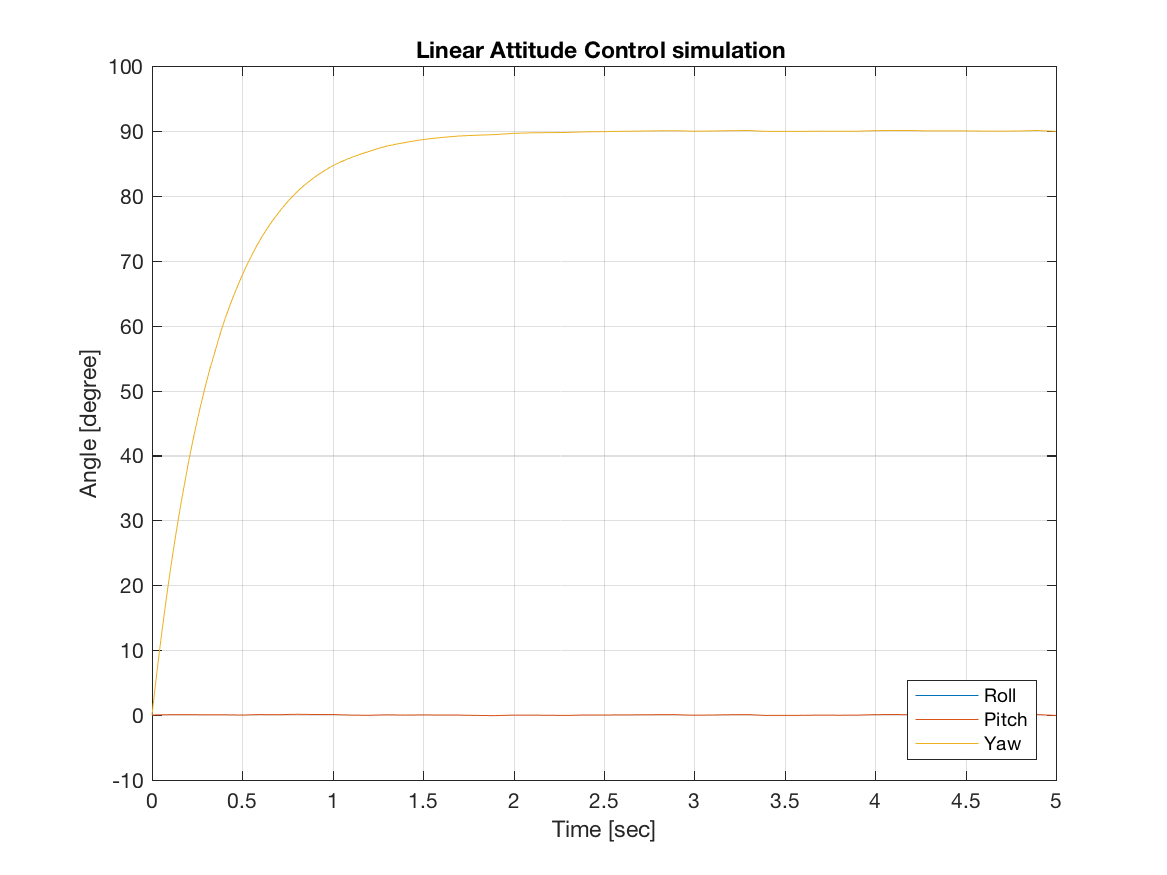
\includegraphics[width=0.45\textwidth]{graphics/yaw_half_pid.png}
    \caption{Simulation Result (Case 6)}
    \label{fig:sim_6}
\end{figure}

\begin{figure}
    \centering
    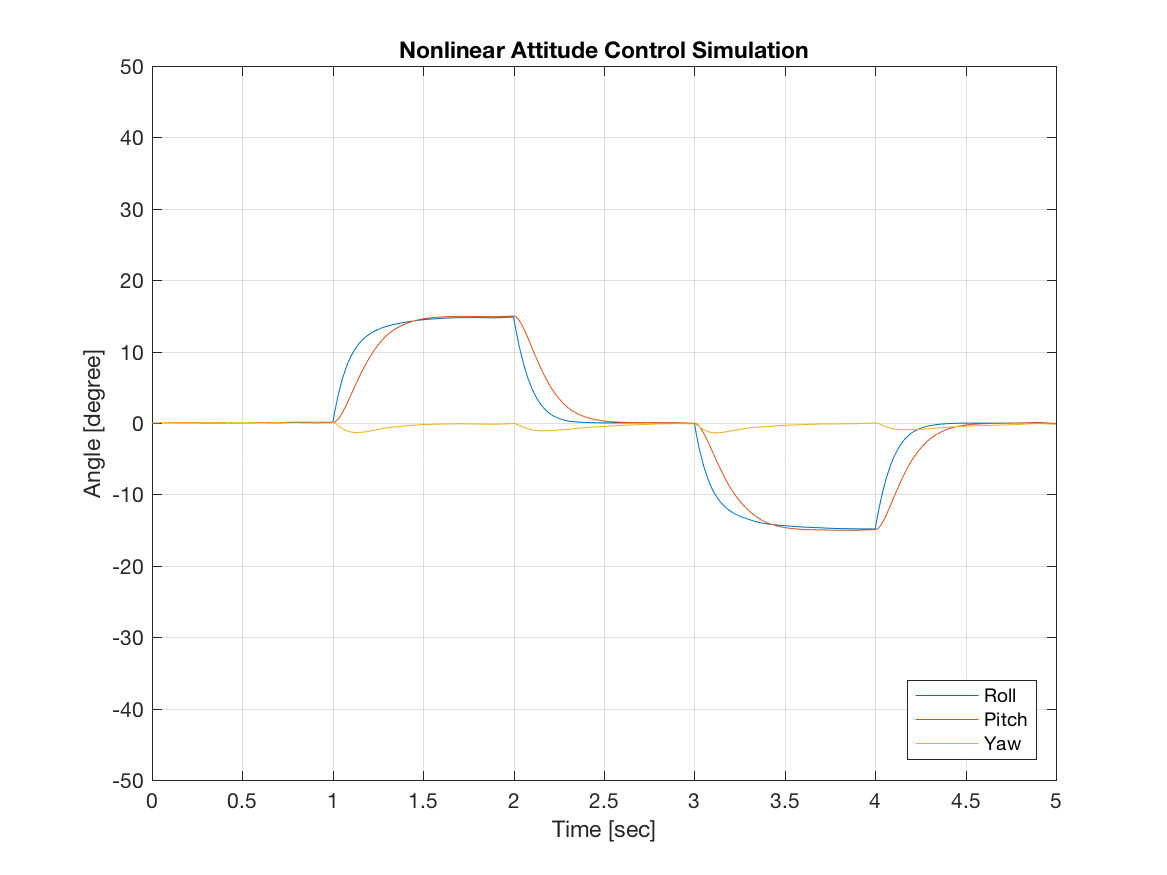
\includegraphics[width=0.45\textwidth]{graphics/custom_01_non.png}
    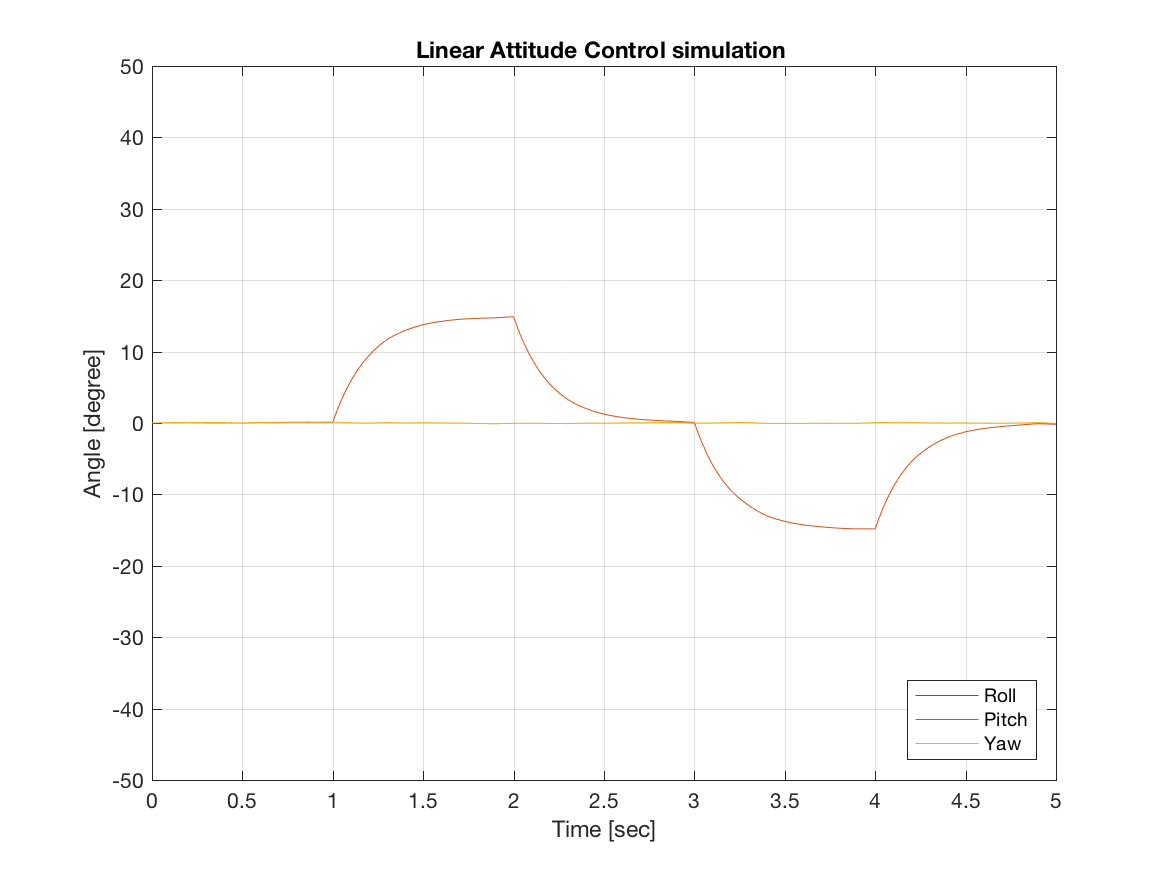
\includegraphics[width=0.45\textwidth]{graphics/custom_01_pid.png}
    \caption{Simulation Result (Case 7)}
    \label{fig:sim_7}
\end{figure}

%%%%%%%%%%%%%%%%%%%%%%%%%%%%%%%%%%%%%%%%%%%%%%%%%%%%%%%%%%%%%%%%%%%%%%%%%%%%%%%%%%%%%%%
\subsection{Discussion}
In most cases, the attitude of the quadrotor converges to the desired attitude faster with the nonlinear control system than it does with the PID linear controller. With roll and pitch changes, the attitude becomes close enough to desired attitude within 0.3 sec at the nonlinear attitude control, and 0.8 sec at the linear attitude control. In the cases of yaw, the rate of convergence is approximately the same for both control systems; the attitude converges to the desired attitude within 1.5 sec. From these results, it can be concluded that the nonlinear attitude controller has the advantage of fast conversion with a guaranteed property robustness \cite{Morgan16}\cite{chung13} . The improvement of the attitude control is expected from global exponential stability of the nonlinear attitude controller. In Figure \ref{fig:sim_7}, the response time of the nonlinear attitude controller is fast enough so that the attitude of the quadrotor stabilize quickly, even with rapid change of desired attitude. Therefore, the nonlinear attitude controller is more suitable for high-agility performance. The deference of response time of the nonlinear attitude control with respect to roll, pitch, and yaw may be caused by the difference of the inertia values along axises, \(I_{xx}\), \(I_{yy}\) and \(I_{zz}\). 

However, the yaw error of the nonlinear attitude control is greater when desired attitude changes in Case 5, than one of the linear attitude control. This is potentially caused by dependency among each angular velocity parameter \(p\), \(q\), and \(r\) at the nonlinear attitude controller. As shown at Equation (\ref{eq:control_law}), each variable cannot be decoupled, while the PID control deals each angular velocity independently. Also, the roll and pitch of the nonlinear attitude controller show different performance, while the the ones of the linear attitude controller are similar to each other. The difference of the inertia among each axis of the body frame possibly causes the asymmetry of the performance.

\section{Flight Experiment}
\label{sec:experiment}

In addition to the simulation study in Section \ref{sec:simulation}, the quadrotor system was tested by experiments to evaluate the nonlinear controller. The flight experiments were executed at the motion capture arena of the Intelligent Robotics Laboratory(IRL) at the University of Illinois at Urbana-Champaign \cite{irl}. The quadrotor was controlled with the outer-loop and inner-loop control stated in Chapter \ref{ch:control_system}. The linear attitude control stated in Section \ref{sec:pid} was also tested with the outer-loop control of Section \ref{sec:outer_loop} to compare with the performance of the nonlinear attitude control. The motion of the quadrotor is recorded by a motion capture system. 
In this chapter, the experimental setup for the evaluation of the quadrotor is stated, and then, the experiment results and discussion about them are followed.

\subsection{Motion Capture Arena}

The quadrotor experiments were done at IRL's motion capture arena for human safety. The arena is equipped with safety facilities for UAVs' flight experiments. The arena is isolated so that the quadrotor does not damage anything out of the arena. In order to limit the range of quadrotors' maneuver and protect them from potential damage, the arena is surrounded by nets. In addition, the floor of the arena is covered with shock absorbing foams to protect the quadrotor from damaging itself. With the setup, potential accidents from the quadrotor's malfunction can be prevented.

Mounted on the ceiling of the four conners of the room, there are installed two motion capture camera; in total eight cameras consists of the motion capture system. The whole arena area is covered by the motion capture range, and the motion capture system measures motion of the object that has reflective motion capture markers on it.

\begin{figure}
    \centering
    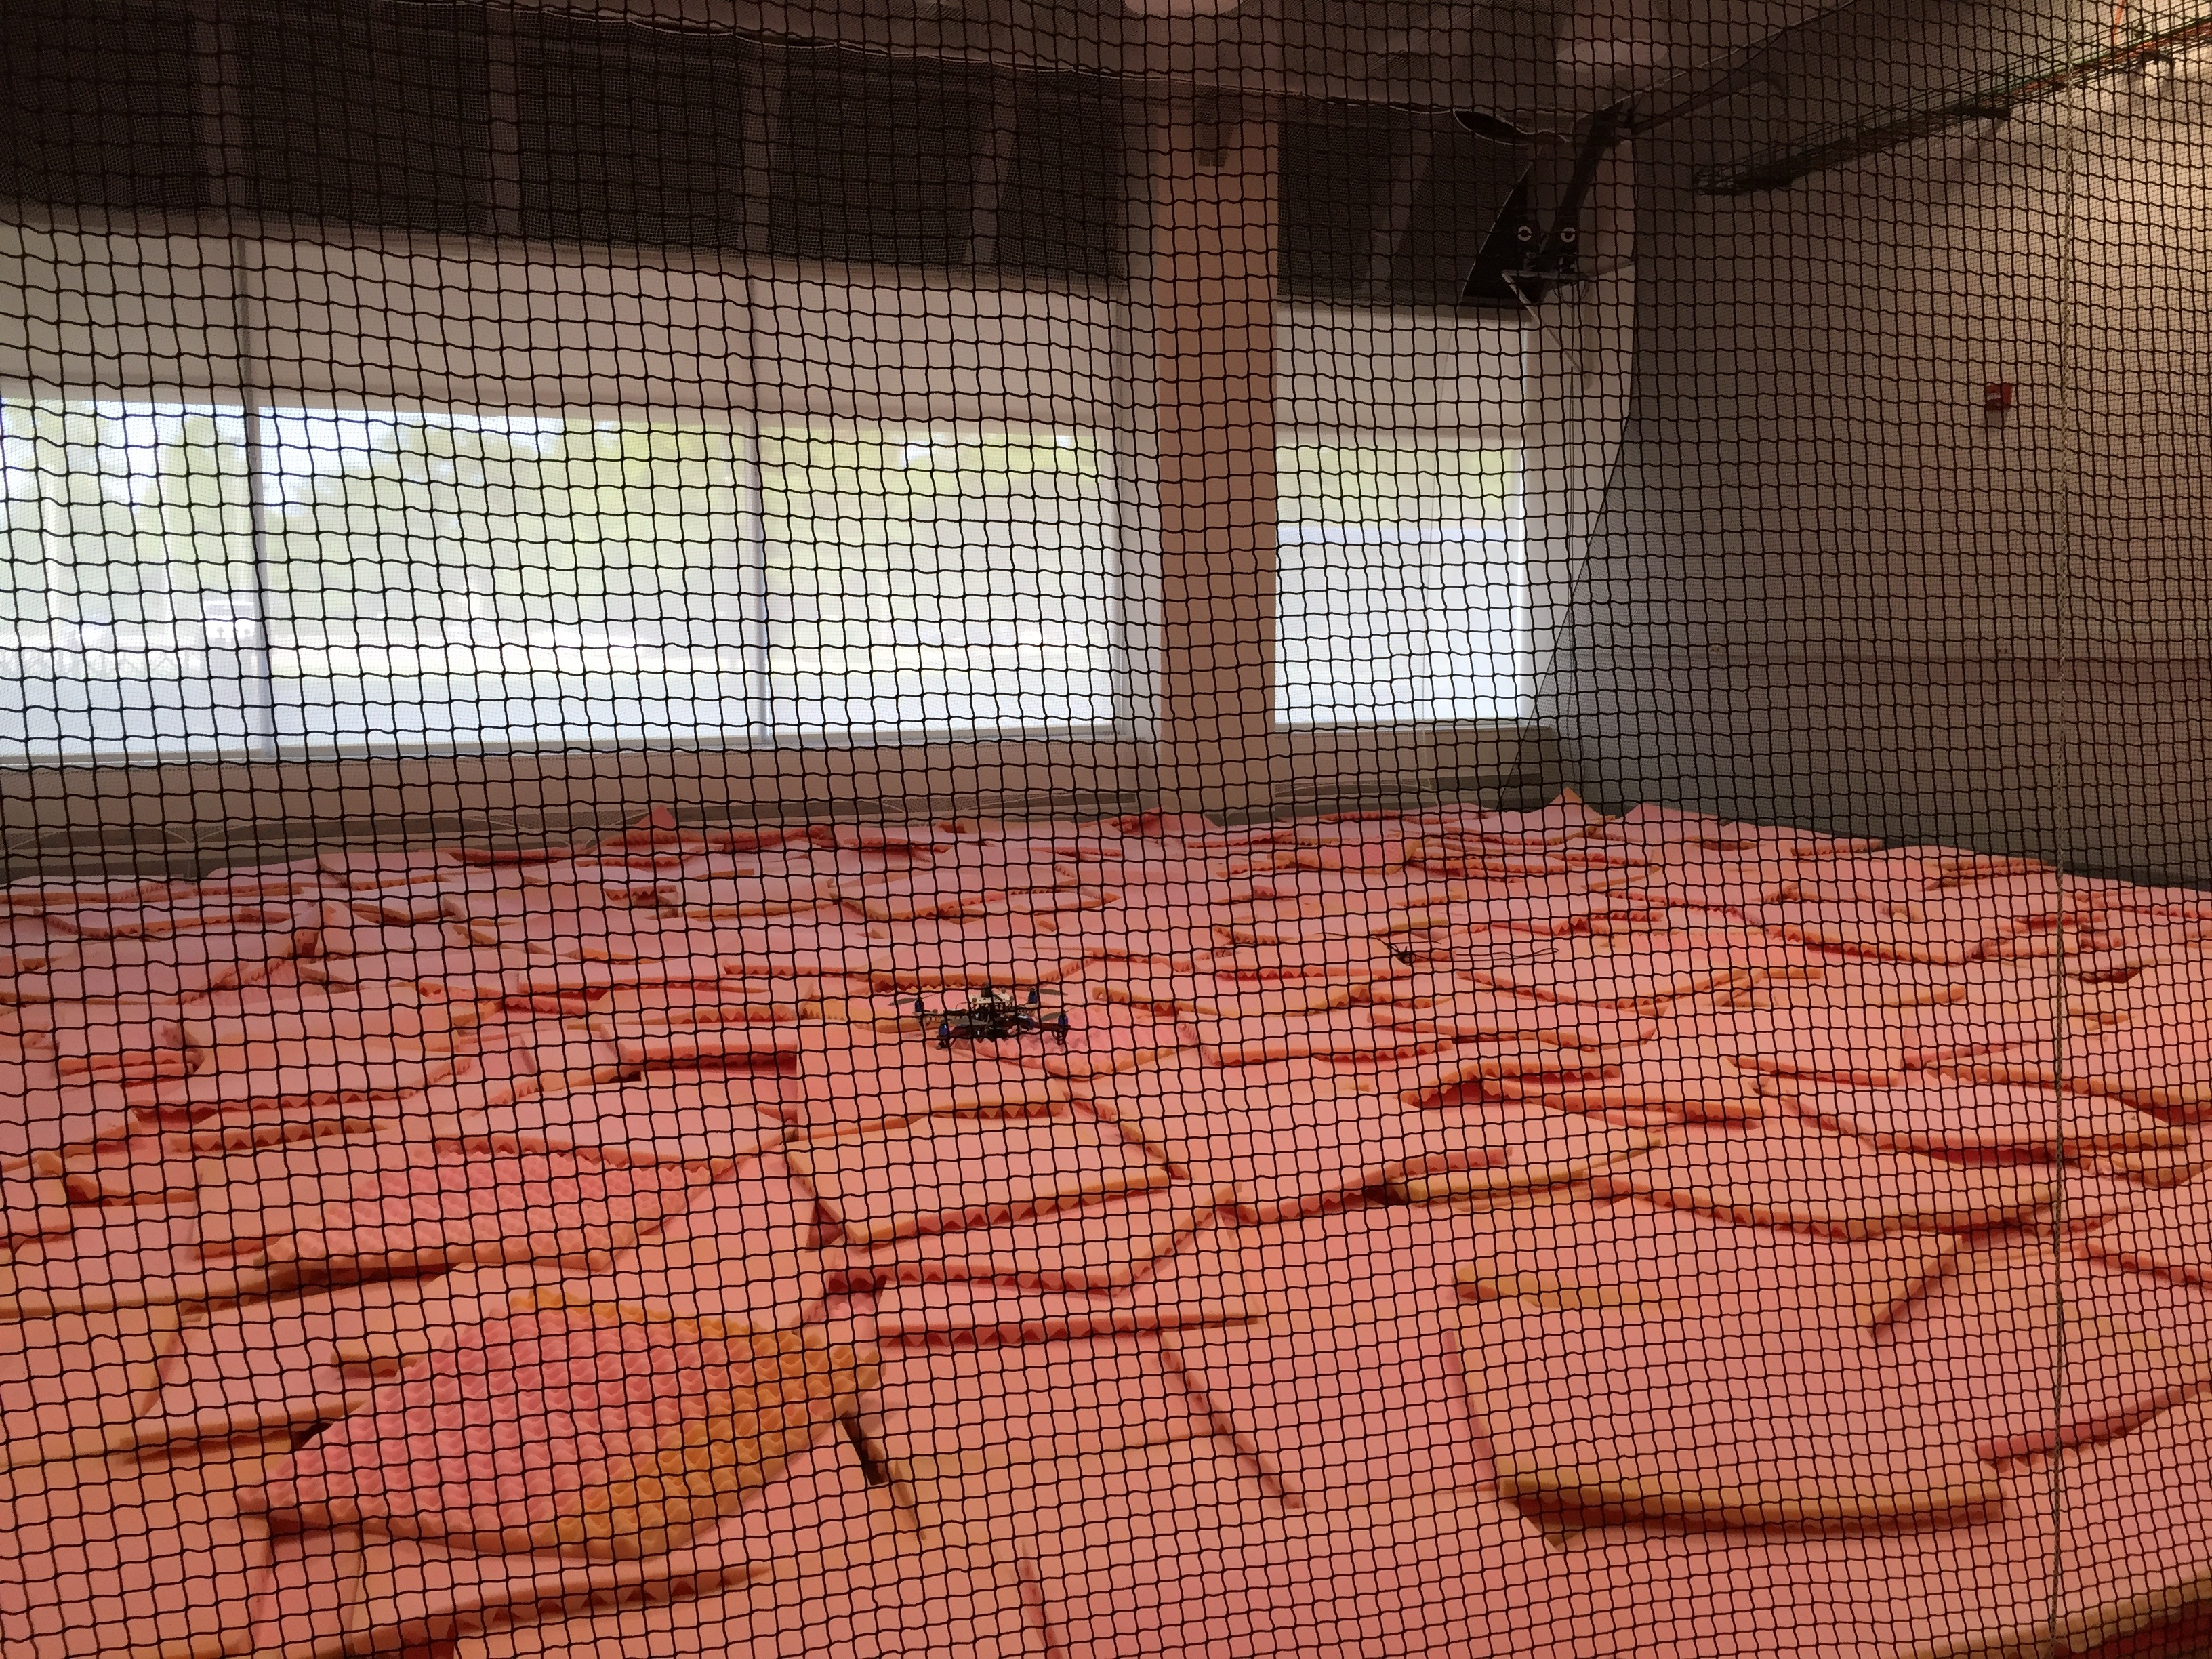
\includegraphics[width=0.8\textwidth]{graphics/arena.jpg}
    \caption{Motion Capture Arena of the Intelligent Robotics Laboratory}
    \label{fig:arena}
\end{figure}

\subsection{Motion Capture System}
IRL's motion capture system consists of 8 Vicon T-series T40S Cameras mounted around the arena. Motion capture cameras of Vicon radiate infrared rays and capture infrared rays reflected from the markers. By synchronizing the pixel coordinate of the reflective markers at multiple motion capture cameras, the motion capture system obtains the position information of the markers \cite{vicon}.

\begin{figure}
    \centering
    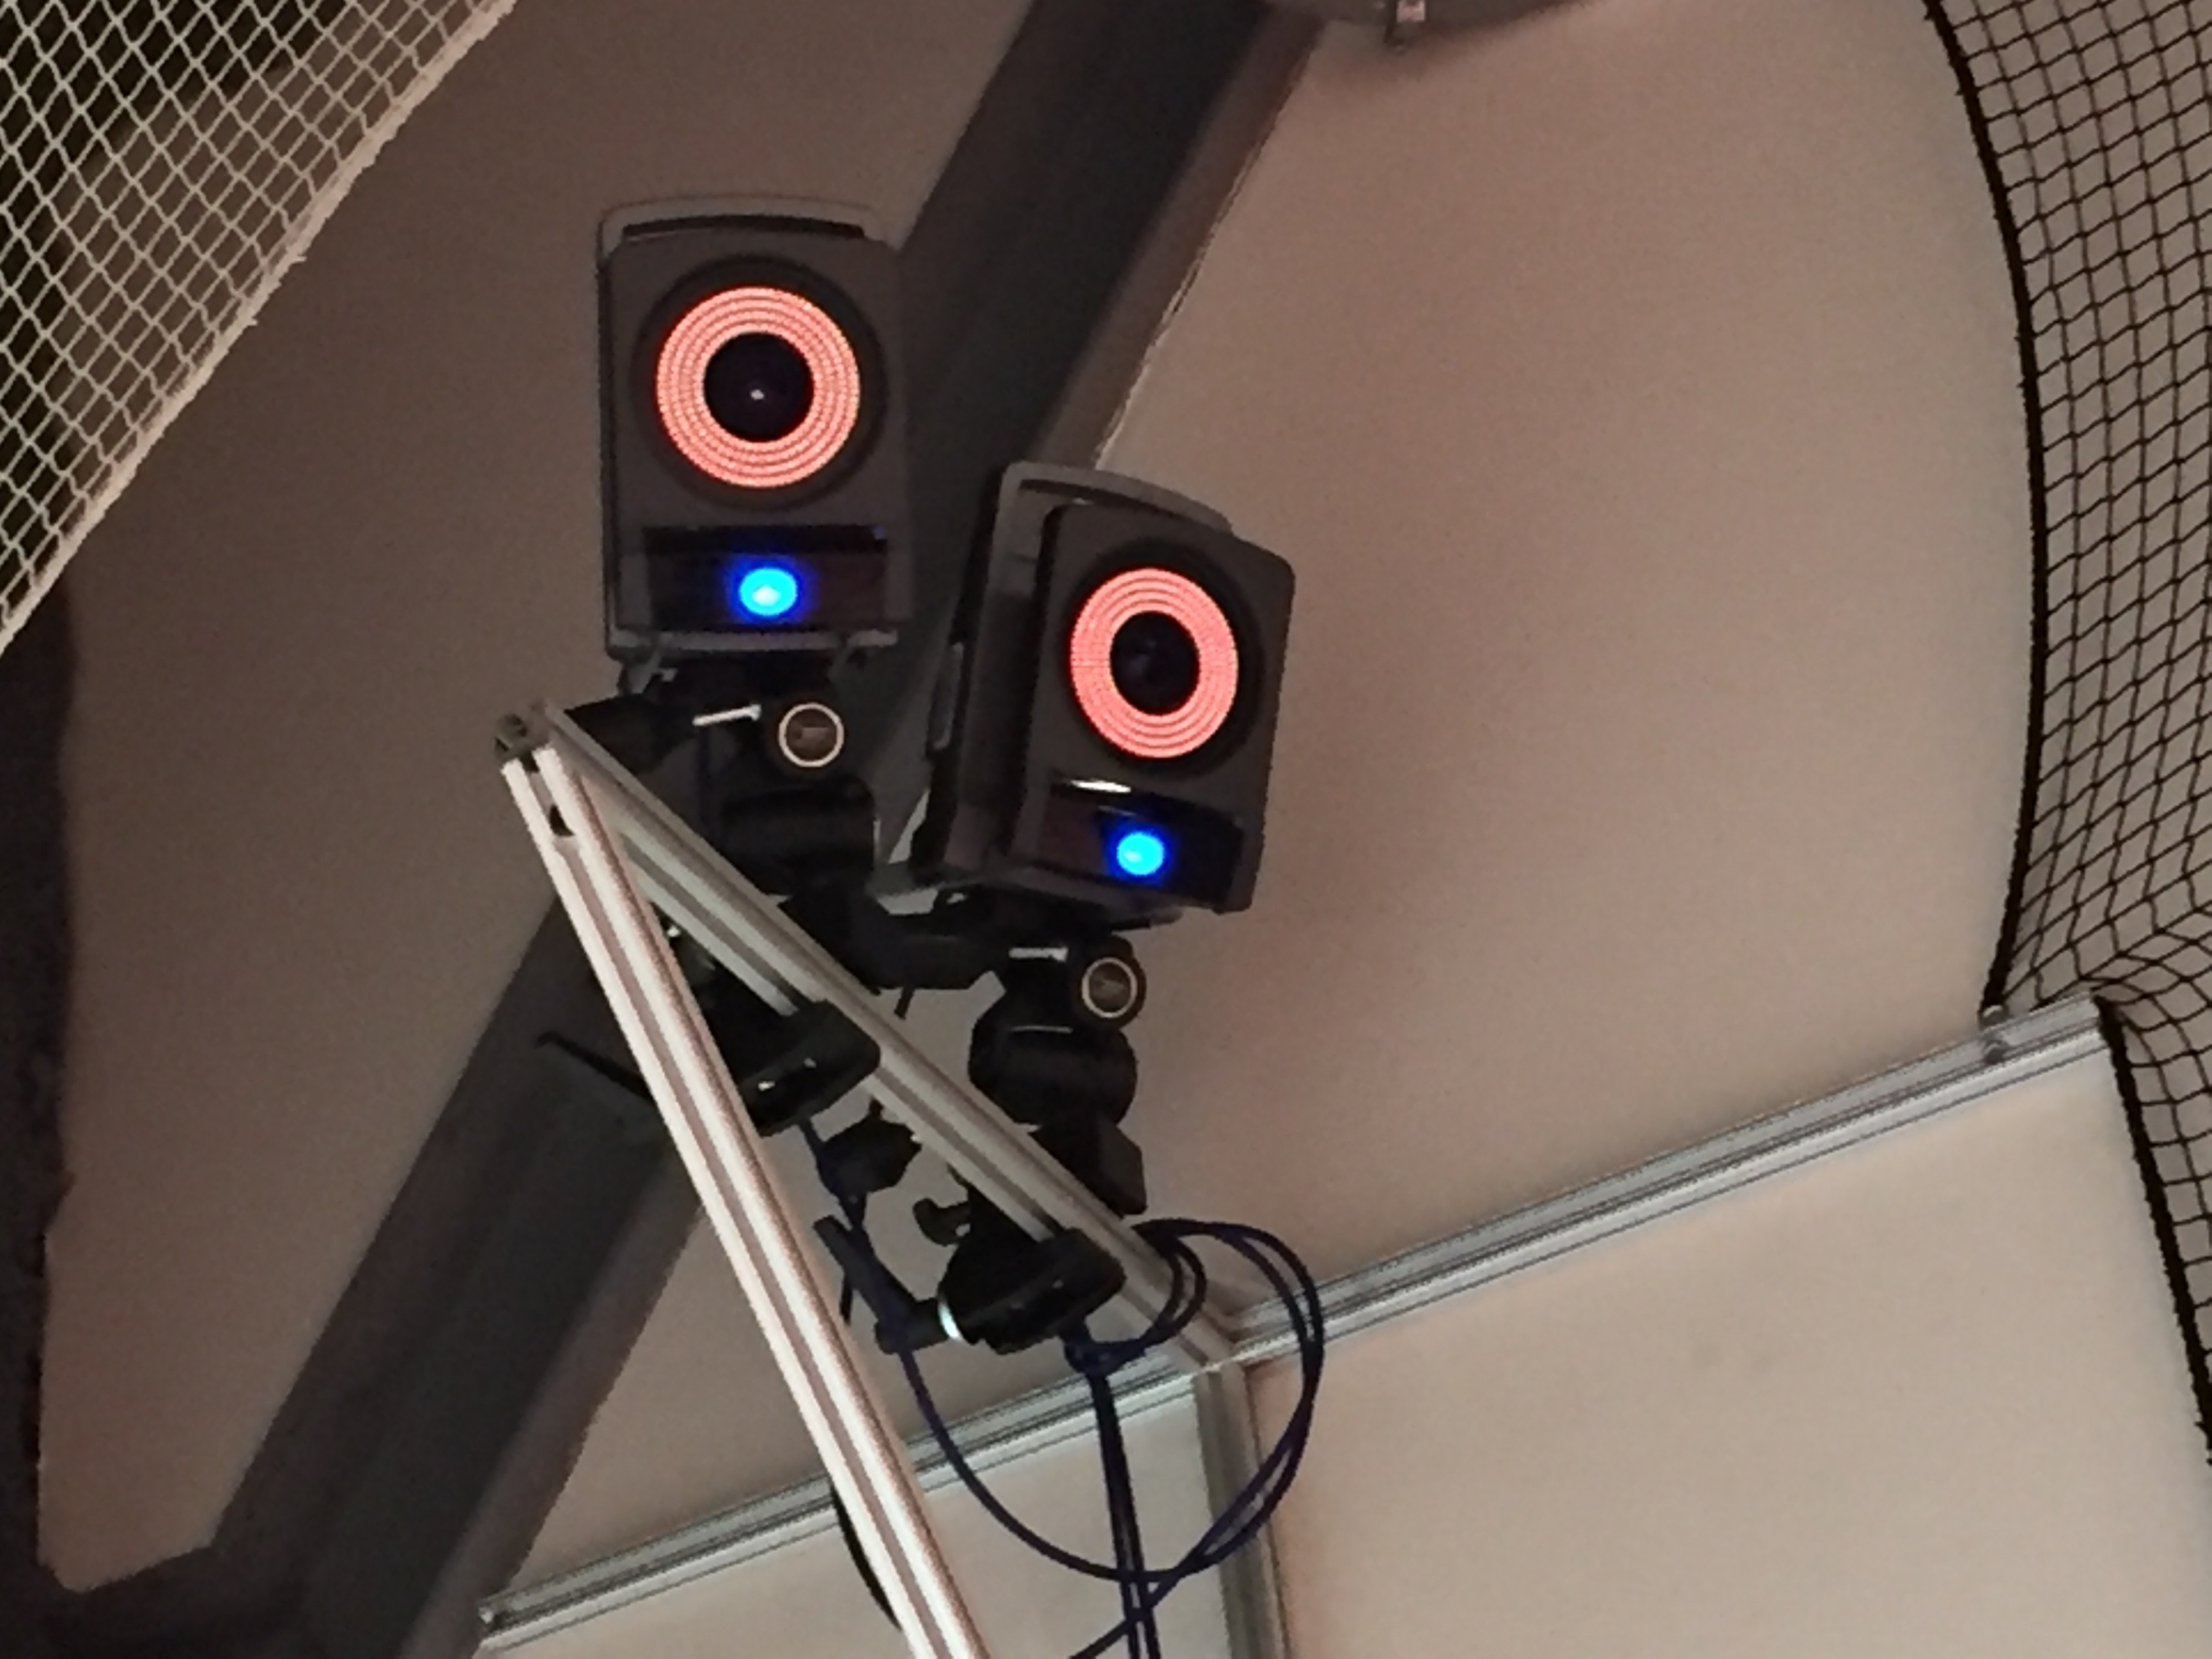
\includegraphics[width=0.5\textwidth]{graphics/vicon_camera.jpg}
    \caption{Vicon Motion Capture Cameras}
    \label{fig:arena}
\end{figure}

Prior to the experiment, it is necessary to register an object that is a rigid body and has multiple markers on it. Then, the motion capture system saves the geometric information of the reflective markers in the database and recognizes the object. In order to measure both the position and attitude of the quadrotor, at least 3 reflector markers must be located on the quadrotor since a plane consist of at least three points. In this experiment, 7 markers are fixed on the quadrotor to guarantee the precision of the motion information; three are located on the quadrotor's legs and the other markers are stick on the top of the quadrotor. To avoid incorrect measurement of the quadrotor's attitude, the markers are installed asymmetrically.

The motion capture system of IRL works with Tracker, a graphic user interface software for Vicon, and Vicon Bridge, a ROS package developed by the autonomous systems laboratory at ETH Zurich are used for streaming the data of the quadrotor position and attitude.

\begin{figure}
    \centering
    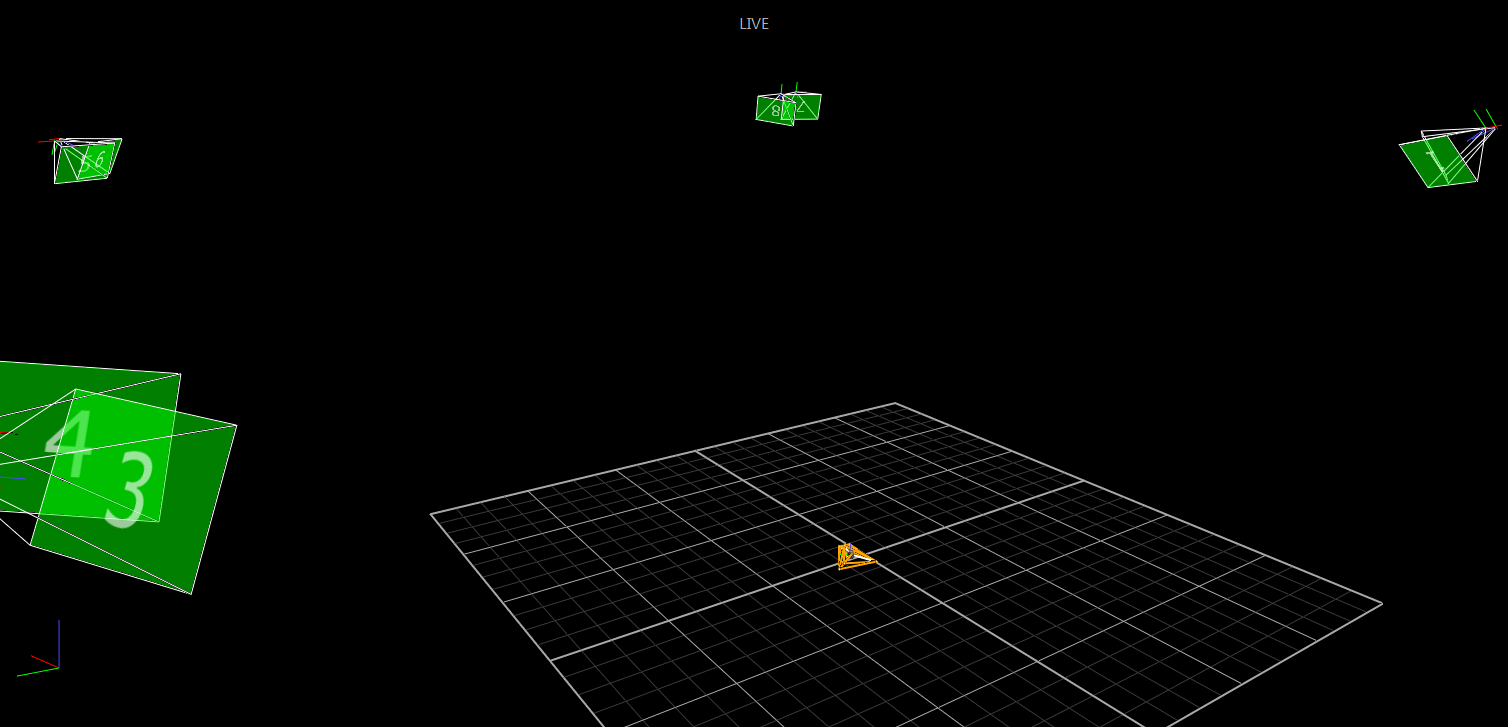
\includegraphics[width=0.8\textwidth]{graphics/tracker.png}
    \caption{Vicon Motion Capture Interface}
    \label{fig:arena}
\end{figure}

\subsection{Experiment Setup}

Prior to experiment, we tuned the control gains of the nonlinear and linear inner-loop controllers, based on the simulated control gains in Section \ref{sec:simulation} and adjusted the gains by multiple flight tests.

In the experiments, the quadrotor was controlled by the PID outer-loop controller described in Section \ref{sec:outer_loop} and either the nonlinear attitude control of Chapter \ref{ch:control_system} or the linear attitude control of Section \ref{sec:pid}. Since it is difficult to set the same desired state of the quadrotor for its position, the position and attitude trajectories for the quadrotor to reach the desired position are used to evaluate performance of each inner-loop controller. Therefore, the desired position of each flight experiment is set to be as far as possible in the motion capture arena from the initial position. The  outer-loop control of the x, y-axis directions is expected to drift since the quadrotor does not include internal position measurement for x, y-axis directions.

The quadrotor's experiments were conducted with focus on control system's stability and agility. First, in order to evaluate the quadrotor's stability, we changed the altitude of the waypoint from 1.8 m to 3 m. The quadrotor first would hover, stabilize its position at the first waypoint, moves to the next waypoint, and land. To evaluate roll agility, we changed the waypoint to either left side or right side from the first waypoint, and then control the quadrotor to land. The waypoint was changed to either forward or backward to validate pitch agility. Finally, yaw performance was also tested by setting desired yaw to be \( \pm {{\pi}\over{2}}\) while the quadrotor hovering on the waypoint. Similarly, as yaw converges to the desired yaw, the quadrotor landed. To summarize, the follow cases were tested.
\begin{enumerate}
\item Take off, change altitude from 1.8m to 3.0m, and land.
\item Take off, move right side, and land.
\item Take off, move left side, and land.
\item Take off, move forward, and land.
\item Take off, move backward, and land.
\item Take off, turn \( \pm {{\pi}\over2}\) to the right, and land.
\item Take off, turn \( \pm {{\pi}\over2}\) to the left, and land.
\end{enumerate}


\subsection{Experiment Results}
All the experimental data are filtered by a low-pass filter and transformed into the coordinate system that is defined in the motion capture system. Also the origin point of each case is defined to be the initial position of the quadrotor. The trajectories and attitude changes over time are plotted in Figures \ref{fig:exp_alt} - \ref{fig:exp_yaw_minus}. Full lines represent the quadrotor's actual trajectories and dashed lines represent the desired position or waypoints.

\begin{figure}
    \centering
    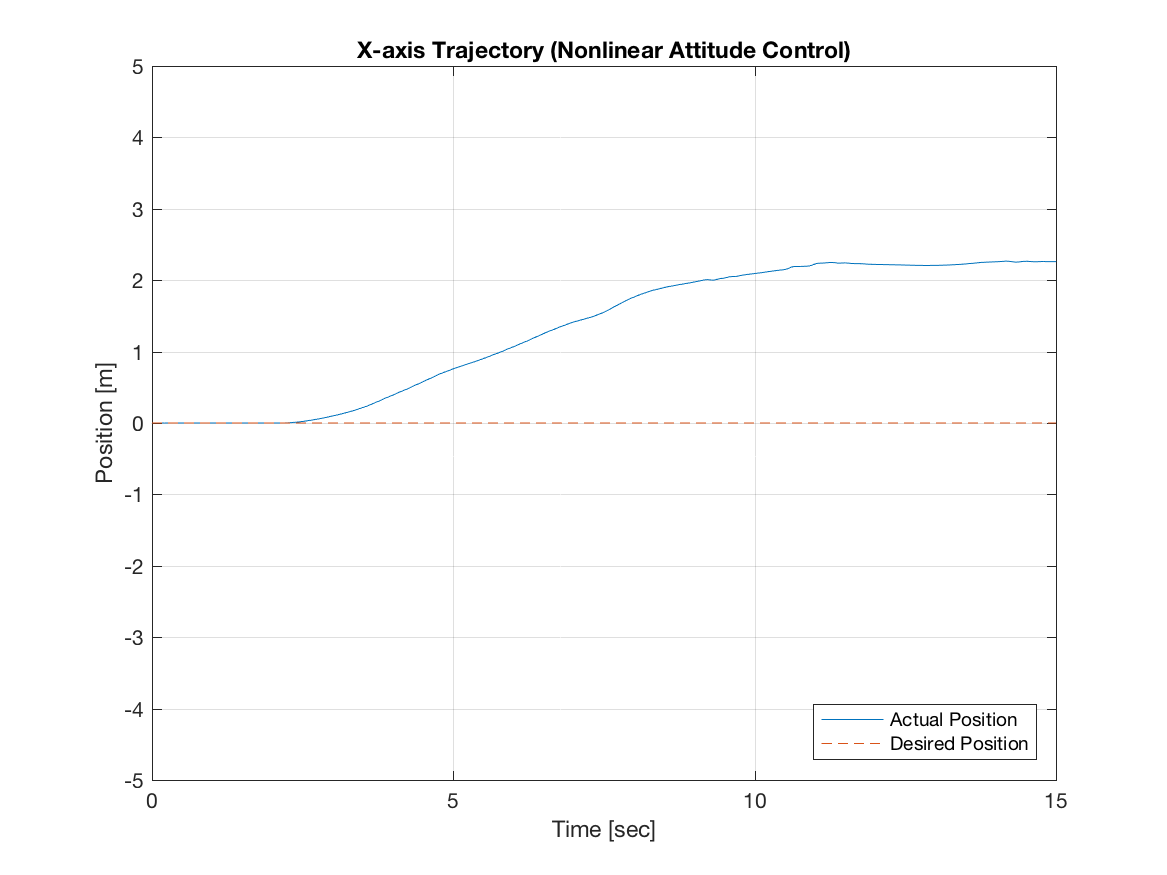
\includegraphics[width=0.45\textwidth]{graphics/experiment_plots/altitude_non_position_x.png}
    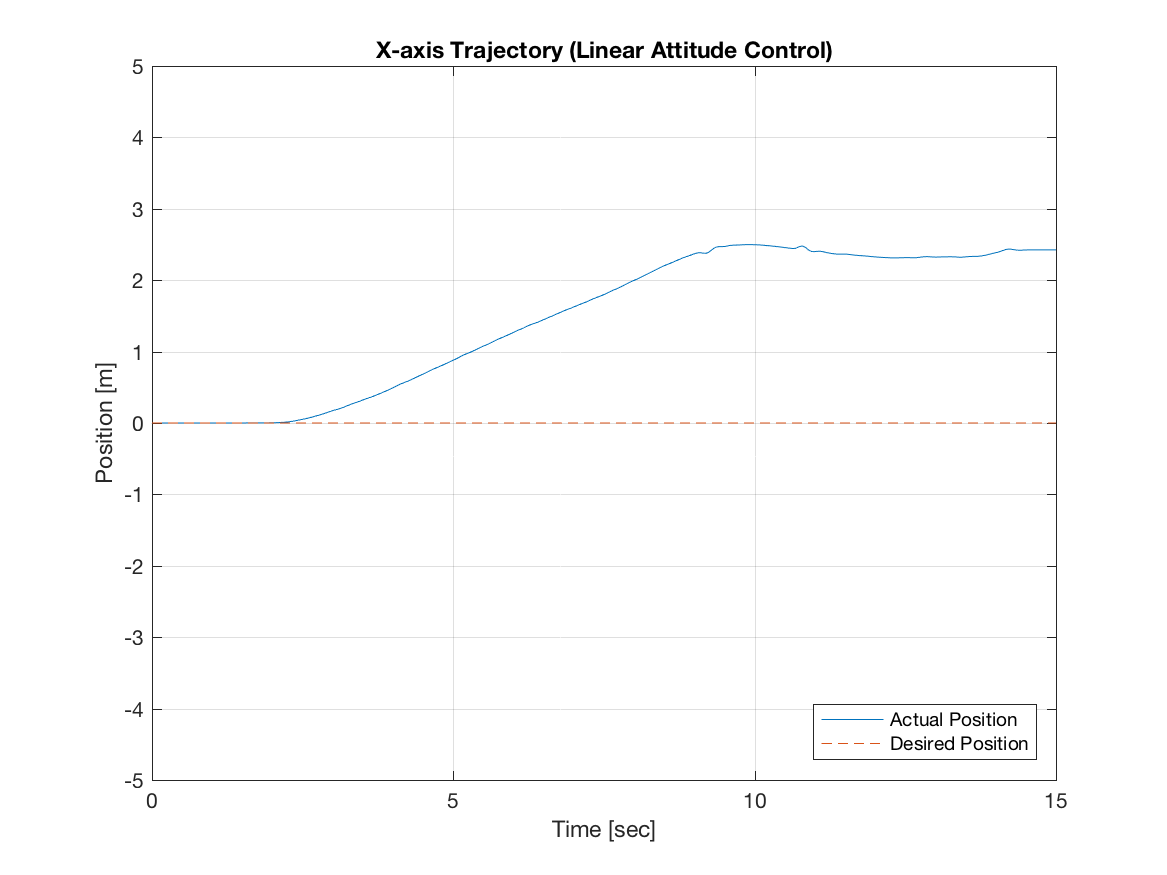
\includegraphics[width=0.45\textwidth]{graphics/experiment_plots/altitude_pid_position_x.png}
    
    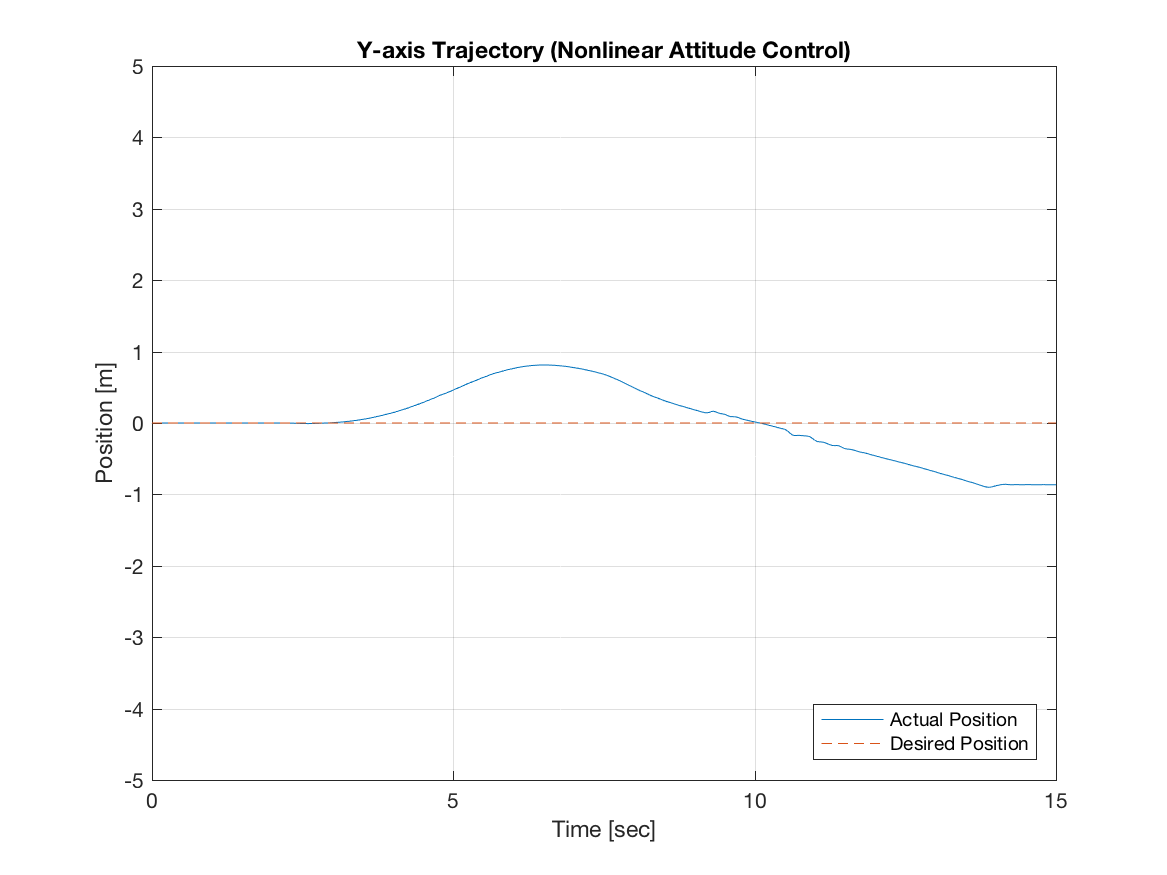
\includegraphics[width=0.45\textwidth]{graphics/experiment_plots/altitude_non_position_y.png}
    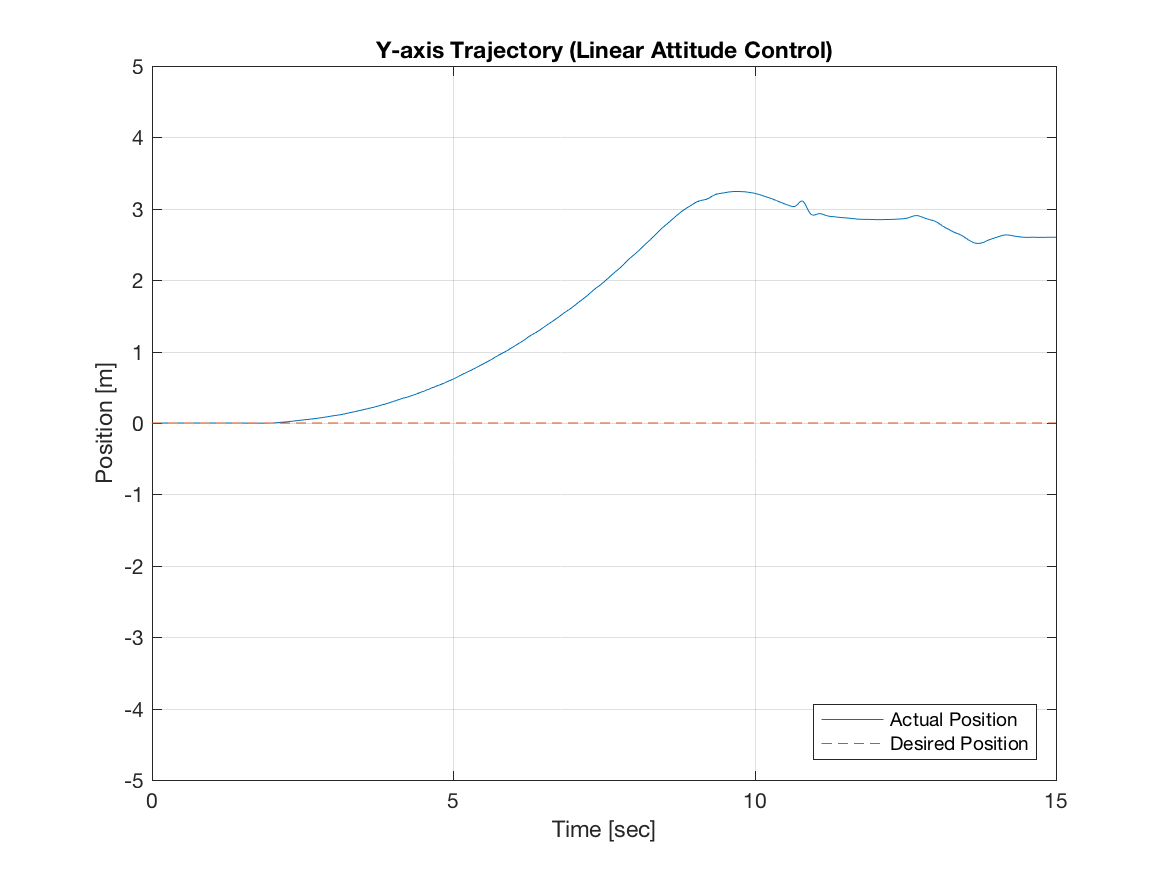
\includegraphics[width=0.45\textwidth]{graphics/experiment_plots/altitude_pid_position_y.png}
    
    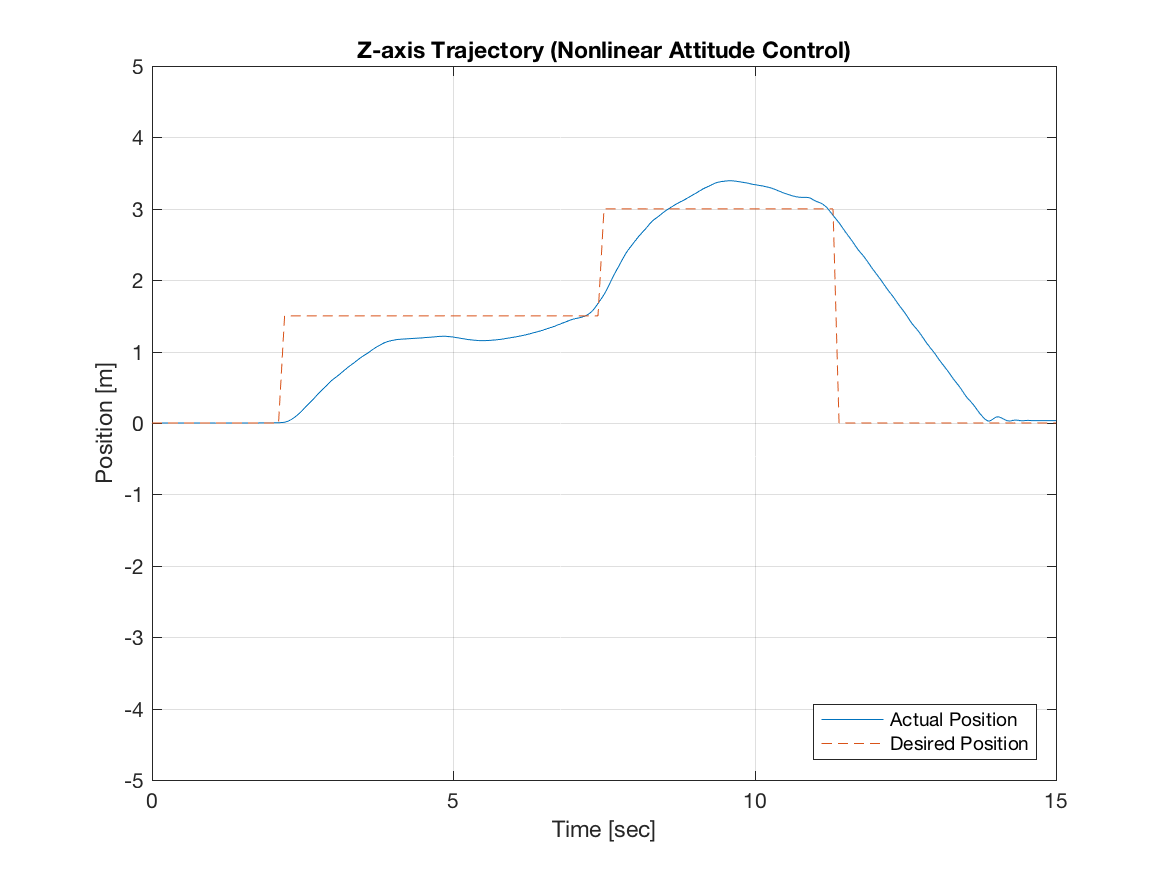
\includegraphics[width=0.45\textwidth]{graphics/experiment_plots/altitude_non_position_z.png}
    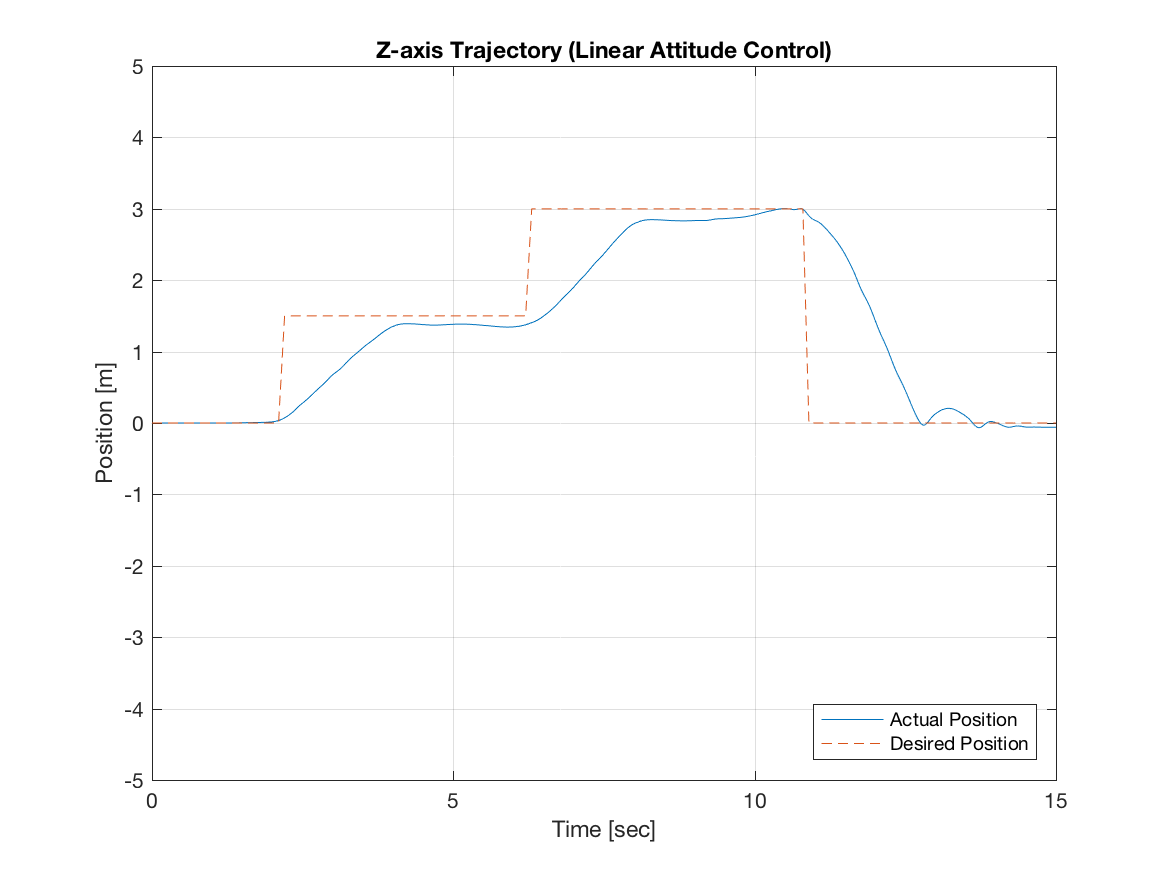
\includegraphics[width=0.45\textwidth]{graphics/experiment_plots/altitude_pid_position_z.png}

    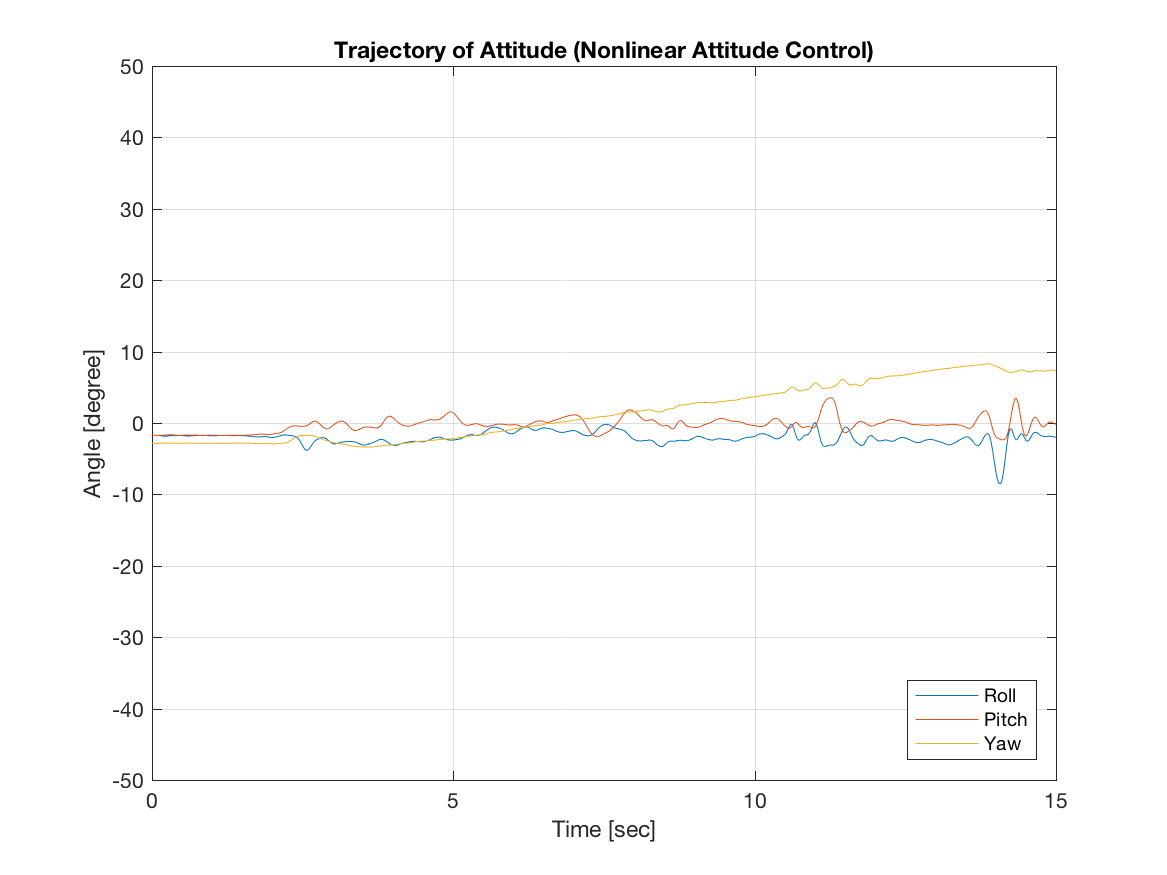
\includegraphics[width=0.45\textwidth]{graphics/experiment_plots/altitude_non_attitude.png}
    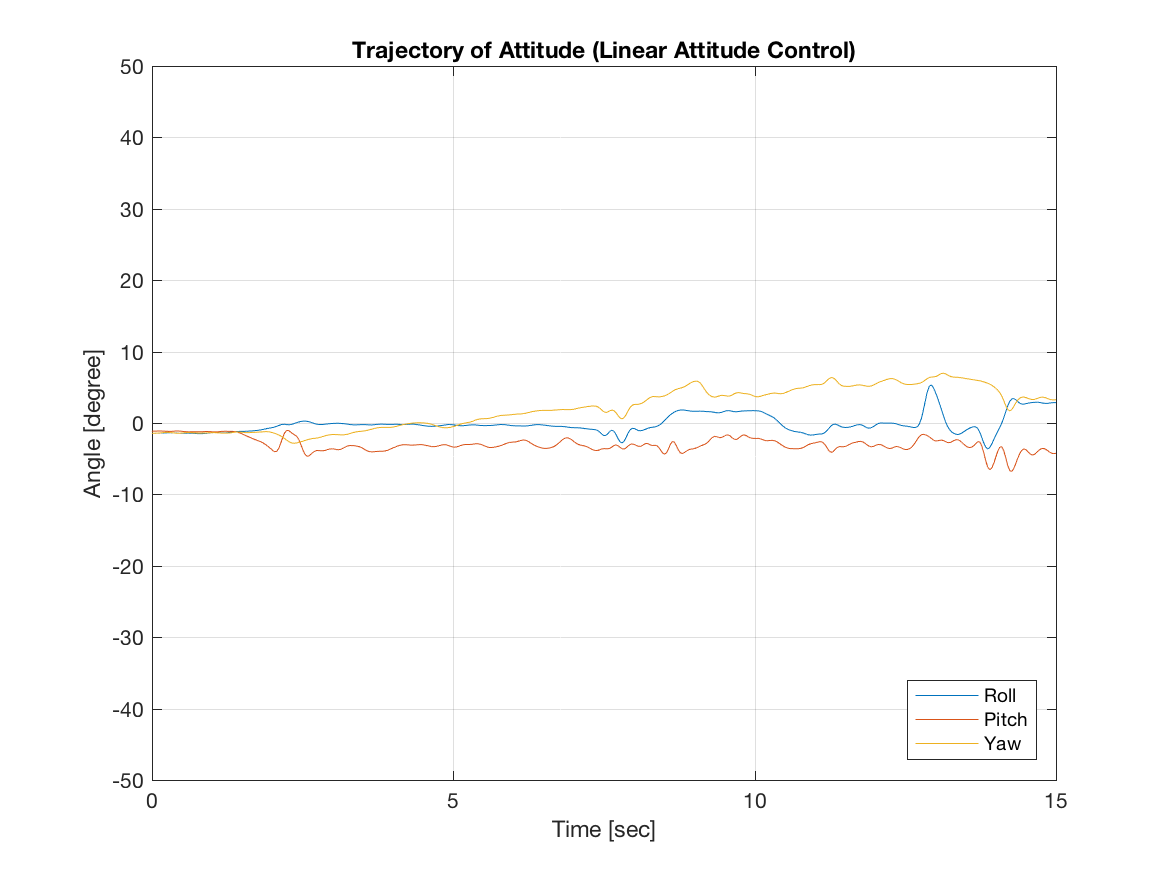
\includegraphics[width=0.45\textwidth]{graphics/experiment_plots/altitude_pid_attitude.png}
    \caption{Experiment Result (Case 1)}
    \label{fig:exp_alt}
\end{figure}

\begin{figure}
    \centering
    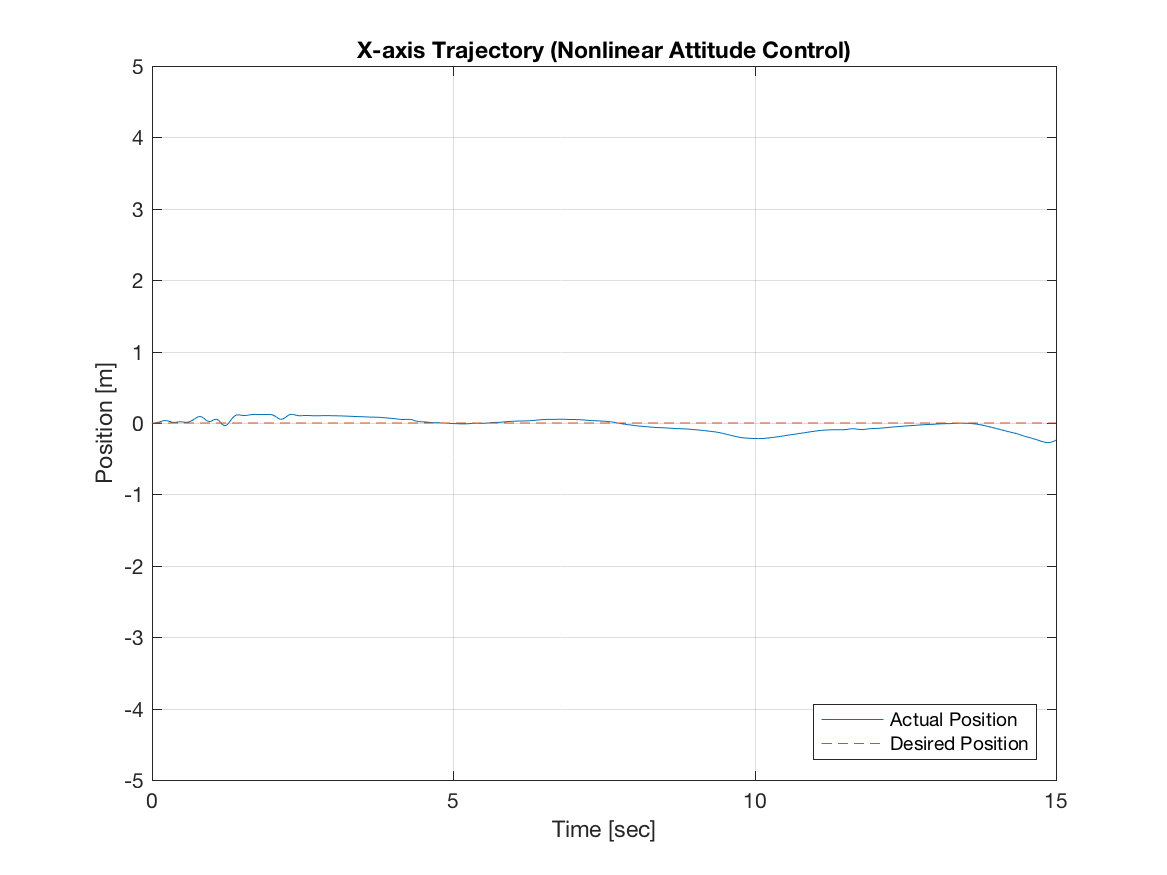
\includegraphics[width=0.45\textwidth]{graphics/experiment_plots/roll_plus_non_position_x.png}
    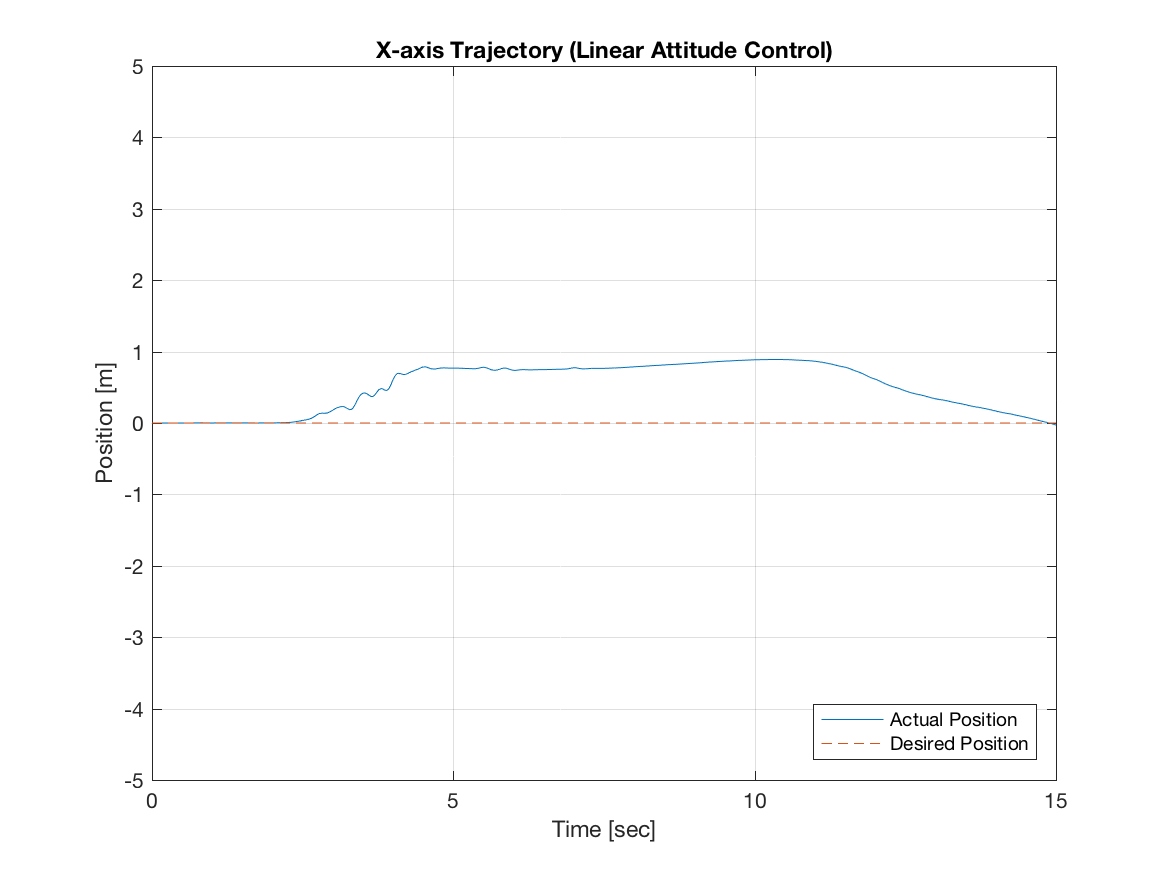
\includegraphics[width=0.45\textwidth]{graphics/experiment_plots/roll_plus_pid_position_x.png}
    
    \includegraphics[width=0.45\textwidth]{graphics/experiment_plots/roll_plus_non_position_y.png}
    \includegraphics[width=0.45\textwidth]{graphics/experiment_plots/roll_plus_pid_position_y.png}
    
    \includegraphics[width=0.45\textwidth]{graphics/experiment_plots/roll_plus_non_position_z.png}
    \includegraphics[width=0.45\textwidth]{graphics/experiment_plots/roll_plus_pid_position_z.png}

    \includegraphics[width=0.45\textwidth]{graphics/experiment_plots/roll_plus_non_attitude.png}
    \includegraphics[width=0.45\textwidth]{graphics/experiment_plots/roll_plus_pid_attitude.png}
    \caption{Experiment Result (Case 2)}
    \label{fig:exp_roll_plus}
\end{figure}

\begin{figure}
    \centering
    \includegraphics[width=0.45\textwidth]{graphics/experiment_plots/roll_minus_non_position_x.png}
    \includegraphics[width=0.45\textwidth]{graphics/experiment_plots/roll_minus_pid_position_x.png}
    
    \includegraphics[width=0.45\textwidth]{graphics/experiment_plots/roll_minus_non_position_y.png}
    \includegraphics[width=0.45\textwidth]{graphics/experiment_plots/roll_minus_pid_position_y.png}
    
    \includegraphics[width=0.45\textwidth]{graphics/experiment_plots/roll_minus_non_position_z.png}
    \includegraphics[width=0.45\textwidth]{graphics/experiment_plots/roll_minus_pid_position_z.png}

    \includegraphics[width=0.45\textwidth]{graphics/experiment_plots/roll_minus_non_attitude.png}
    \includegraphics[width=0.45\textwidth]{graphics/experiment_plots/roll_minus_pid_attitude.png}
    \caption{Experiment Result (Case 3)}
    \label{fig:exp_roll_minus}
\end{figure}

\begin{figure}
    \centering
    \includegraphics[width=0.45\textwidth]{graphics/experiment_plots/pitch_plus_non_position_x.png}
    \includegraphics[width=0.45\textwidth]{graphics/experiment_plots/pitch_plus_pid_position_x.png}
    
    \includegraphics[width=0.45\textwidth]{graphics/experiment_plots/pitch_plus_non_position_y.png}
    \includegraphics[width=0.45\textwidth]{graphics/experiment_plots/pitch_plus_pid_position_y.png}
    
    \includegraphics[width=0.45\textwidth]{graphics/experiment_plots/pitch_plus_non_position_z.png}
    \includegraphics[width=0.45\textwidth]{graphics/experiment_plots/pitch_plus_pid_position_z.png}

    \includegraphics[width=0.45\textwidth]{graphics/experiment_plots/pitch_plus_non_attitude.png}
    \includegraphics[width=0.45\textwidth]{graphics/experiment_plots/pitch_plus_pid_attitude.png}
    \caption{Experiment Result (Case 4)}
    \label{fig:exp_pitch_plus}
\end{figure}

\begin{figure}
    \centering
    \includegraphics[width=0.45\textwidth]{graphics/experiment_plots/pitch_minus_non_position_x.png}
    \includegraphics[width=0.45\textwidth]{graphics/experiment_plots/pitch_minus_pid_position_x.png}
    
    \includegraphics[width=0.45\textwidth]{graphics/experiment_plots/pitch_minus_non_position_y.png}
    \includegraphics[width=0.45\textwidth]{graphics/experiment_plots/pitch_minus_pid_position_y.png}
    
    \includegraphics[width=0.45\textwidth]{graphics/experiment_plots/pitch_minus_non_position_z.png}
    \includegraphics[width=0.45\textwidth]{graphics/experiment_plots/pitch_minus_pid_position_z.png}

    \includegraphics[width=0.45\textwidth]{graphics/experiment_plots/pitch_minus_non_attitude.png}
    \includegraphics[width=0.45\textwidth]{graphics/experiment_plots/pitch_minus_pid_attitude.png}
    \caption{Experiment Result (Case 5)}
    \label{fig:exp_pitch_minus}
\end{figure}

\begin{figure}
    \centering
    \includegraphics[width=0.45\textwidth]{graphics/experiment_plots/yaw_plus_non_position_x.png}
    \includegraphics[width=0.45\textwidth]{graphics/experiment_plots/yaw_plus_pid_position_x.png}
    
    \includegraphics[width=0.45\textwidth]{graphics/experiment_plots/yaw_plus_non_position_y.png}
    \includegraphics[width=0.45\textwidth]{graphics/experiment_plots/yaw_plus_pid_position_y.png}
    
    \includegraphics[width=0.45\textwidth]{graphics/experiment_plots/yaw_plus_non_position_z.png}
    \includegraphics[width=0.45\textwidth]{graphics/experiment_plots/yaw_plus_pid_position_z.png}

    \includegraphics[width=0.45\textwidth]{graphics/experiment_plots/yaw_plus_non_attitude.png}
    \includegraphics[width=0.45\textwidth]{graphics/experiment_plots/yaw_plus_pid_attitude.png}
    \caption{Experiment Result (Case 6)}
    \label{fig:exp_yaw_plus}
\end{figure}

\begin{figure}
    \centering
    \includegraphics[width=0.45\textwidth]{graphics/experiment_plots/yaw_minus_non_position_x.png}
    \includegraphics[width=0.45\textwidth]{graphics/experiment_plots/yaw_minus_pid_position_x.png}
    
    \includegraphics[width=0.45\textwidth]{graphics/experiment_plots/yaw_minus_non_position_y.png}
    \includegraphics[width=0.45\textwidth]{graphics/experiment_plots/yaw_minus_pid_position_y.png}
    
    \includegraphics[width=0.45\textwidth]{graphics/experiment_plots/yaw_minus_non_position_z.png}
    \includegraphics[width=0.45\textwidth]{graphics/experiment_plots/yaw_minus_pid_position_z.png}

    \includegraphics[width=0.45\textwidth]{graphics/experiment_plots/yaw_minus_non_attitude.png}
    \includegraphics[width=0.45\textwidth]{graphics/experiment_plots/yaw_minus_pid_attitude.png}
    \caption{Experiment Result (Case 7)}
    \label{fig:exp_yaw_minus}
\end{figure}

\subsection{Discussion}
As discussed above, the quadrotor does not have internal position measurement of the x,y-axis directions, and therefore, there are drifts along the x,y-axis directions in every case. The position estimator uses integration of values from the internal accelerometer. Errors are accumulated by iteration, and therefore, position drifts are not avoidable. The errors caused by drifts are usually less severe with the nonlinear control system introduced in Chapter \ref{ch:control_system}. The drift occurs especially when the quadrotor takes off and lands. Dynamic factors, such as corrosion between the quadrotor's leg and the ground, are potential reasons of drifts at taking off and landing. Also, the aerodynamic model may be different near the ground and, therefore, may cause drifts as well.

In most cases, x, y-axis position errors of the linear controller are greater than the errors of the nonlinear controller. In Case 1, the y-axis drift is less than 1 m with the nonlinear control system while the error is about up to 3 m with the linear control system, and the x-axis drifts of both controllers are similar. In Cases 4 and 5, the x, y-axis position errors with the nonlinear attitude control are bounded up to 1 m, but the errors of the linear attitude control grow up to 3 m. The x, y-axis errors show similar tendencies in Cases 2 and 3. However, compared with Cases 4 and 5, the errors with the linear control system do not exceed 2 m. In Cases 6 and 7, the x, y-axis error rates of the linear control system are twice greater than the error rates of the nonlinear control system. We were not able to further reduce the position errors of the PID attitude control by tuning the gains. From these results, we can conclude that the nonlinear control system has an advantage of superior performance, compared with the linear control system.

However, the nonlinear control system does not seem to have an advantage with respect to z-axis position over an conventional PID control system. There are increasing and decreasing of altitude while the quadrotor changes its attitude, but z-axis position errors of both controllers are less than 0.5 m in most cases. As mentioned in Chapter \ref{ch:system}, the Pixhawk autopilot is equipped with an internal barometer to measure altitude and frequently corrects position estimation of double integration of acceleration. Therefore, with more precise altitude estimation, the quadrotor stabilizes its altitude better than its x,y-axis position.

In addition, time for the quadrotor to reach desired position with the nonlinear control system is approximately the same as the one with the linear attitude control since there is an upper limit of desired velocity. However, as shown in Figures \ref{fig:exp_roll_plus} - \ref{fig:exp_pitch_minus}, the quadrotor with the nonlinear control system responses fast and reaches to the maximum velocity, while it moves more smoothly with the linear control system. Also, as shown in Figures \ref{fig:exp_yaw_plus} and \ref{fig:exp_yaw_minus}, yaw control is more stabilized with the nonlinear control system. These support globally exponentially stability of the nonlinear attitude control in Section \ref{sec:inner_loop} and the results of simulation in Section \ref{sec:simulation} that the nonlinear control converges to desired attitude faster than PID attitude control does since the quadrotor's attitude affects the direction of acceleration. Therefore, we can conclude that the nonlinear control system also has an advantage of its stability.

However, the \(K_{\omega}\) and \(\Lambda\) gains should be further tuned for the nonlinear control to draw a definitive conclusion between the nonlinear control method and the PID attitude controller method. Also, there are constant yaw drifts at both control systems in Cases 2 and 3, Yaw angle increases when the quadrotor moves to right, while the yaw angle decreases when the quadrotor moves to the left. We can presume that the misalignment of the internal gyroscope or the different output curves of the DC motors caused the drifts.

\chapter{Vision-based Position Estimator}
\label{ch:vision_based_control}

As discussed in Section \ref{sec:experiment}, the lack of precise position measurement causes the quadrotor's drift. Therefore, the quadrotor must be equipped with proper position measurement, such as a GPS sensor and a video sensor, for its stable autonomous operation. A simple and light position estimator based on image processing is introduced in this chapter. We assumed the case that the quadrotor hovers above four markers located on the floor.

This chapter consists of the following contents. First, the camera distortion model used in the system is stated. Then, the image processes used for detecting markers are described. Finally, a geometric relation between the pixel coordinates of the markers and the quadrotor's position is described, and a method to estimate the quadrotor position is introduced.

\section{Camera Calibration}
%http://www.vision.caltech.edu/bouguetj/calib_doc/htmls/parameters.html
An image from a camera is often distorted by mechanical factors; radial distortion caused by the shape of the lens, and tangential distortion caused by the angle and the distance between the video sensor and the lens. The camera used in the quadrotor system has \({120}^{\circ}\) view angle, and due to its wide angle, radial distortion is especially severe. In order to collect precise image data from the camera, calibration is required.

In this research, camera calibration is processed by GML C++ Camera Calibration Toolbox, developed by the Graphics and Media Laboratory at Moscow State University \cite{gml}. The calibration toolbox is based on the polynomial camera model. Let \( {\boldsymbol {\text x}}_d = ({\text x}_d, {\text y}_d) \) be the normalized point coordinate with distortion, and \( {\boldsymbol {\text x}} =  ({\text x}, {\text y}) \) be the normalized point coordinate without distortion. Then, the model is given as the below equation \cite{caltech_calib}.\\
\begin{equation}
\label{eq:distortion_model}
\begin{aligned}
{\text x}_d = (1 + {k_c}_1 {\text r}^2 + {k_c}_2 {\text r}^4 + {k_c}_5 {\text r}^6 ) {\boldsymbol {\text x}} + 
\begin{bmatrix}
2 {k_c}_3 {\text x} {\text y} + {k_c}_4 ({\text r}^2 + 2 {\text x}^2) \\
{k_c}_3 ({\text r}^2 + 2 {\text y}^2 + 2 {k_c}_4 {\text x} {\text y})
\end{bmatrix}
\end{aligned}
\end{equation}\\
where \({\boldsymbol k}_c = ( {k_c}_1, {k_c}_2, {k_c}_3, {k_c}_4, {k_c}_5 )\) is the distortion coefficients of the camera and \(\text r\) is defined with respect to \(\text x\) and \(\text y\) as the below equation.
\begin{equation}
\begin{aligned}
{\text r}^2 = {\text x}^2 + {\text y}^2
\end{aligned}
\end{equation}\\
In Equation (\ref{eq:distortion_model}), the first term of the right side represents radial distortion, and the second term of the right side represents tangential distortion. In addition to distortion, the pixel coordinates of the projection \(p\) is given as,
\begin{equation}
\begin{aligned}
p = K_K {\boldsymbol {\text x}}_d
\end{aligned}
\end{equation}
where \(K_K\) is the camera matrix, defined as,
\begin{equation}
\begin{aligned}
K_K = 
\begin{bmatrix}
{f_c}_1 & \alpha_c {f_c}_1 & {c_c}_1 \\
0 & {f_c}_2 & {c_c}_2 \\
0 & 0 & 1
\end{bmatrix}
\end{aligned}
\end{equation}\\
\({f_c}_1\), \({f_c}_2\) are the focal distances and \(\alpha_c\) is the angle between the x and y sensor axes. Therefore, by measuring the distortion coefficients  \( \boldsymbol{k}_c\) and the camera matrix \(K_K\), the undistorted coordinate \( \boldsymbol{\text x} \) can be restored from the raw pixel coordinate \(p\). Figure \ref{fig:camera_calibration} shows the results of the marker image restored from the raw image by camera calibration.
\begin{figure}
    \centering
    \includegraphics[width=0.45\textwidth]{graphics/raw.png}
    \includegraphics[width=0.45\textwidth]{graphics/undistorted.png}
    \caption{Camera Calibration (Left: Raw Image, Right: Restored Image)}
    \label{fig:camera_calibration}
\end{figure}

\section{Marker Detection}
Marker detection can be achieved by multiple image processes. First of all, a monochrome image is used. In order to decrease noise and find clear borders, the image is filtered by the Gaussian filter and thresholded. Then, the morphology closing transformation is processed to restore holes on the borders. Once the image has clean borders, the markers are detected with their contours. To be specific, the "findContours" function of OpenCV 2.4 is used for the process of finding contours \cite{opencv}.

From the above image processes, the markers of the image are detectable. However, due to environmental factors, such as lightness and floor state, empty coordinates possibly be detected as markers. Therefore, the following strategy is applied in the system. Consider the case that more than 4 coordinates \(p_i\) are detected as markers. Since the reference makers are fixed and clustered, and wrongly-detected coordinates are few, usually zero or, at most, two, markers are located close to the center of the set of candidates. By using this method, incorrect candidates are excluded easily.

The result of each step is shown in Figure \ref{fig:threshold} - \ref{fig:result}. The white circles in Figure \ref{fig:result} point the centers of the image markers.

\begin{figure}
    \centering
    \includegraphics[width=0.45\textwidth]{graphics/threshold.png}
    \caption{Gaussian-filtered and Thresholded Image}
    \label{fig:threshold}
\end{figure}

\begin{figure}
    \centering
    \includegraphics[width=0.45\textwidth]{graphics/contour.png}
    \caption{Restoration of Borders}
    \label{fig:contour}
\end{figure}


\begin{figure}
    \centering
    \includegraphics[width=0.45\textwidth]{graphics/result.png}
    \caption{Final Result of Marker Detection}
    \label{fig:result}
\end{figure}


\section{Position Estimation}
\begin{figure}
    \centering
    \includegraphics[width=0.8\textwidth]{graphics/scheme.pdf}
    \caption{Schematic Diagram of the Position Estimation}
    \label{fig:scheme}
\end{figure}
Let  \(\vec{ h} \) be the normal vector of the camera's orientation. Then, from Equation (\ref{eq:z_inv_eta}),  it can be represented with respect to the quadrotor's attitude \( {\boldsymbol \eta} \) as,
\begin{equation}
\begin{aligned}
{\vec h} ( {\boldsymbol \eta} ) & =  Z^{-1} 
\begin{bmatrix}
0 \\
0 \\
-1
\end{bmatrix}
 = 
\begin{bmatrix}
\sin{\theta} \\
- \sin{\phi} \cos{\theta} \\
- \cos{\phi} \cos{\theta}
\end{bmatrix}\\
\end{aligned}
\end{equation}
Let \( \boldsymbol A \) be the area of the polygon in the inertial frame, and \(\vec{l_i} \) be the relative position of a marker according to the position of the camera. Then, the projection of  \(\boldsymbol A \) is represented as below equation \cite{Haralick94}. \\
\begin{equation}
\label{eq:projection}
\begin{aligned}
{\vec h} \cdot { \boldsymbol A} & = {1 \over 2}(\vec{l_2} - \vec{l_1}) \times (\vec{l_4} - \vec{l_1}) + {1 \over 2}(\vec{l_4} - \vec{l_3}) \times (\vec{l_2} - \vec{l_3}) \\
& = {1 \over 2}(\vec{l_1} \times \vec{l_2} + \vec{l_2} \times \vec{l_3}  + \vec{l_3} \times \vec{l_4} + \vec{l_4} \times  \vec{l_1}) 
\end{aligned}
\end{equation}
From perspective projection of the camera, the relative position \(\vec{l_i}\) is represented with respect to the normalized pixel coordinate \( {\boldsymbol p}_i\), \\
\begin{equation}
\begin{aligned}
\vec{l_i} =  {d\over {\vec{h} \cdot ({R_{\psi}}^{-1} {\boldsymbol p}_i}) } {R_{\psi}}^{-1} {\boldsymbol p}_i 
\end{aligned}
\end{equation}
where \( d \) is the perpendicular distance from the camera to the plane of the markers, and it is unknown. For convenience of computation, define the composite coordinate,\\
\begin{equation}
\begin{aligned}
{{\boldsymbol p}_{\psi}}_i = {R_{\psi}}^{-1} {\boldsymbol p}_i 
\end{aligned}
\end{equation}
Then, Equation (\ref{eq:projection}) can be written as, \\
\begin{equation}
\begin{aligned}
{\vec h} \cdot { \boldsymbol A} & = {{ \Gamma d} \over 2} 
\end{aligned}
\end{equation}
where \(\Gamma \) is a composite value defined as,\\
\begin{equation}
\begin{aligned}
\Gamma = 
\left(
{{{{{\boldsymbol p}_{\psi}}_1} \times {{{\boldsymbol p}_{\psi}}_2}} \over {({\vec{h} \cdot {{\boldsymbol p}_{\psi}}_1})({\vec{h} \cdot {{\boldsymbol p}_{\psi}}_2})}} + 
{{{{{\boldsymbol p}_{\psi}}_2} \times {{{\boldsymbol p}_{\psi}}_3}} \over {({\vec{h} \cdot {{\boldsymbol p}_{\psi}}_2})({\vec{h} \cdot {{\boldsymbol p}_{\psi}}_3})}} +
{{{{{\boldsymbol p}_{\psi}}_3} \times {{{\boldsymbol p}_{\psi}}_4}} \over {({\vec{h} \cdot {{\boldsymbol p}_{\psi}}_3})({\vec{h} \cdot {{\boldsymbol p}_{\psi}}_4})}} +
{{{{{\boldsymbol p}_{\psi}}_4} \times {{{\boldsymbol p}_{\psi}}_1}} \over {({\vec{h} \cdot {{\boldsymbol p}_{\psi}}_4})({\vec{h} \cdot {{\boldsymbol p}_{\psi}}_1})}} \right) 
\end{aligned}
\end{equation}
From the above equation, \( d \) is computed as,\\
\begin{equation}
\begin{aligned}
{d} = \sqrt{{2 {\vec h} \cdot { \boldsymbol A} }\over{\Gamma}} 
\end{aligned}
\end{equation}
and therefore, the relative position of the camera according to the markers' center is given as, \\
\begin{equation}
\label{eq:relative_position}
\begin{aligned}
{\tilde {\boldsymbol r}}
& = - {1\over 4} (\vec{l_1} + \vec{l_2} + \vec{l_3} + \vec{l_4}) \\
& =  - {d \over 4} \left( { {{{\boldsymbol p}_{\psi}}_1}\over {\vec{h} \cdot {{\boldsymbol p}_{\psi}}_1} }+ { {{{\boldsymbol p}_{\psi}}_2}\over {\vec{h} \cdot {{\boldsymbol p}_{\psi}}_2} } + { {{{\boldsymbol p}_{\psi}}_3}\over {\vec{h} \cdot {{\boldsymbol p}_{\psi}}_3} } +{ {{{\boldsymbol p}_{\psi}}_4}\over {\vec{h} \cdot {{\boldsymbol p}_{\psi}}_4} } \right)
\end{aligned}
\end{equation}

Since the relative position calculated from the markers is noisy, the Kalman filter is applied to estimate and correct the value. A value computed by Equation (\ref{eq:relative_position}) passes through the Kalman filter, and the filtered value is used as relative position of the quadrotor, corresponding to the markers.

\section{Evaluation Experiment}
\subsection{Experimental Setup}
The vision-based position estimator was tested by experiments. The experiments ware also executed at the IRL motion capture arena. The quadrotor was not armed, and the autopilot only publishes the sensor values to the onboard companion computer via UART. The algorithm was run by the companion computer in real-time. In order to evaluate the results, the Vicon motion capture system of the arena was used, and streaming data from the position estimator and the motion capture system are compared. As described at Section \ref{sec:experiment}, the Vicon system detects the reflective markers on the quadrotor and measures the position of the quadrotor in its own coordinate system. The image markers used in the experiment for the position estimation are shown in Figure \ref{fig:markers}. Each image marker is a 15cm-diameter-circle and its center is located about 45 cm away from the ones of its neighbors. The placement of the image markers forms a square. The origin of the inertial coordinate system is set to be at the center of the image markers.

\begin{figure}
    \centering
    \includegraphics[width=0.45\textwidth]{graphics/markers.png}
    \caption{Image Markers for the Evaluation}
    \label{fig:markers}
\end{figure}

\subsection{Results}
All the position data from the motion capture system are filtered by a low-pass filter and transformed into the coordinate system defined by the motion capture system. The position data from the position estimator were processed by a real-time Kalman filter. The results of the experiments are shown in Figures \ref{fig:cam_x} - \ref{fig:cam_z}. Each figure shows the position measurements of both the above vision-based position estimator and the motion capture system.

\begin{figure}
    \centering
    \includegraphics[width=0.45\textwidth]{graphics/cam_x.png}
    \caption{Experiment Result of the Position Estimator (x-axis Position)}
    \label{fig:cam_x}
    \vspace{1cm}
    \includegraphics[width=0.45\textwidth]{graphics/cam_y.png}
    \caption{Experiment Result of the Position Estimator (y-axis Position)}
    \label{fig:cam_y}
    \vspace{1cm} 
    \includegraphics[width=0.45\textwidth]{graphics/cam_z.png}
    \caption{Experiment Result of the Position Estimator (z-axis Position)}
    \label{fig:cam_z}
\end{figure}

\subsection{Discussion}
As shown in Figure \ref{fig:cam_x} - \ref{fig:cam_z}, the errors of the position estimator are about 0.3 m when the position of camera moves slowly. Therefore, it can be concluded that the position estimator works roughly correctly. Considering the experimental results of x, y-axis position errors at Subsection \ref{sec:experiment} are up to 3 m and the errors grow as time pasts, the vision-based estimator is expected to improve the quadrotor's navigation.

However, as Figure \ref{fig:cam_z} shows, the position estimator is not able to reflect small change of the position among z-axis less than 0.5 m. Therefore, the position estimator is more suitable for slow flight, rather than agile performance. In addition, the camera may not capture the image markers if the camera is too close to the ground. The absence of the markers on the image frame can be a critical reason of the failure of position estimation. The problem potentially happens when the quadrotor has high roll or pitch angle, and therefore, it necessary to develop a system that deals with temporary failure of marker detection. 

\chapter{Conclusion}
\label{ch:conclusion}

In this research, a dynamic model-based nonlinear attitude control was developed. First, we developed a quadrotor system testbed that satisfies the requirements for potential future research. Then, we studied the dynamics of the quadrotor and developed a nonlinear inner-loop attitude controller based on the model. Further, by characterizing the motor dynamics and analyzing the propeller aerodynamics, we developed an advanced model of the quadrotor that allows more stable and agile control. Based on the model, we developed a nonlinear attitude controller and applied it to the quadrotor system.
 
The nonlinear control that has been developed in this research has an advantage of globally exponentially stability. Therefore, if a proper dynamic model for the quadrotor can be defined, the control law is expected to allow better performance of the quadrotor. In order to validate the maneuver advantage of the nonlinear controller, the quadrotor's performance was evaluated by both simulations and experiments. The flight performance of the quadrotor with the nonlinear attitude control is compared with the performance of a conventional PID attitude control, and it was verified that the nonlinear attitude control is superior in stability and agility, and therefore, effective for a quadrotor UAVs. By further tuning the gains of the nonlinear controller, we can expect to clearly establish the benefits of the proposed nonlinear control method.

However, in order to develop fully-autonomous system for the quadrotor, it is necessary to install position measurement on the quadrotor. Therefore, in Chapter \ref{ch:vision_based_control}, a computationally-efficient vision-based position estimator was designed. Since the position estimator is executable in real-time, it is expected to be used in the quadrotor system so that the quadrotor corrects accumulated position errors.

As for future works, synchronized with the nonlinear attitude control, the application of the motion planning and guidance is expected to further improve the quadrotor's performance \cite{motion_planning}\cite{Morgan16}\cite{Morgan14}. Especially for path planning of rapid maneuvering, high nonlinearity of an aerial vehicle is challenging which possibly exacerbates and restricts its maneuver \cite{Paranjape15}. However, the nonlinear attitude controller developed in this research is expected to guarantee stability and allow fast maneuver. Also, in this research, the motor dynamics is approximated by experiments, but precise modeling of a motor would increase the robustness of the inner-loop control as well. The nonlinear attitude inner-loop controller has an advantage of stability in terms of angular velocity as well as attitude, and therefore, the nonlinear quadrotor system is expected to be applied to a quadrotor's acrobatic flight that requires high response speed of angular velocity.


\appendix*

\include{Appendix.tex}

\backmatter

\begin{thebibliography}{9}

\bibitem{icao16} 
I. C. A. O. Cir,
"328 AN/190",
Unmanned Aircraft Systems (UAS) Circular,
2011.

\bibitem{Hoffmann07} 
G. M. Hoffmann, H. Huang, S. L. Waslander, and C. J. Tomlin,
"Quadrotor Helicopter Flight Dynamics and Control: Theory and Experiment?"
\textit{Proc. of the AIAA Guidance, Navigation, and Control Conference},
 vol. 2. Aug 2007.

\bibitem{Michael02}
N. Michael, S. Shen, K. Mohta, Y. Mulgaonkar, V. Kumar, K. Nagatni, Y. Okada, S. Kiribayashi, K. Otake, K. Yashida, and K. Ohno
"Collaborative Mapping of an Earthquake-Damaged Building via Ground and Aerial Robots," 
\textit{Journal of Field Robotics},
vol. 29, no. 5, Aug. 2012, pp. 832-841.

\bibitem{Chambers11}
A. Chambers, S. Achar, S. Nuske, J. Rehder, B. Kitt, L. Chamberlain, J. Haines, S. Scherer, and S. Singh,
"Perception for a River Mapping Robot,"
\textit{In Intelligent Robots and Systems (IROS), 2011 IEEE/RSJ International Conference on}, 
IEEE, Sep 2011, pp. 227-234.

\bibitem{Raffo08}
G. V. Raffo, M. G. Ortega, and F. R. Rubio,
"Backstepping/Nonlinear \({\mathscr{H}}_{\infty}\) Control for Path Tracking of a Quadrotor Unmanned Aerial Vehicle,"
\textit{In American Control Conference, 2008}, 
IEEE, Jun 2008, pp. 3356-3361.

\bibitem{Morgan16}
D. Morgan, G. P. Subramanian, S. . Chung, and F. Y. Hadaegh,
"Swarm Assignment and Trajectory Optimization Using Variable-Swarm, Distributed Auction Assignment and Sequential Convex Programming," 
\textit{The International Journal of Robotics Research},
Feb. 2016. 0278364916632065.

\bibitem{Mallikarjunan12}
S. Mallikarjunan, B. Nesbitt, E. Kharisov, E. Xargay, N. Hovakimyan, and Chengyu Cao,
"L1 Adaptive Controller for Attitude Control of Multirotors,"
\textit{In AIAA Guidance, Navigation and Control Conference, Minneapolis}, 
AIAA-2012-4831. 2012.

 \bibitem{Diao11}
 C. Diao, B. Xian, Q. Yin, W. Zeng, H. Li, and Y. Yang,
"A Nonlinear Adaptive Control Approach for Quadrotor UAVs,"
 \textit{In Control Conference (ASCC), 2011 8th Asian}, 
 IEEE, May 2011, pp. 223-228.
 
 \bibitem{Ritz11}
 R. Ritz, Robin, M. Hehn, S. Lupashin, and R. D'Andrea.
"Quadrocopter Performance Benchmarking Using Optimal Control,"
\textit{In Intelligent Robots and Systems (IROS), 2011 IEEE/RSJ International Conference on}, 
 IEEE, Sep 2011, pp. 5179-5186.
 
 \bibitem{Mellinger12}
 D. Mellinger, N. Michael, and V. Kumar,
"Trajectory Generation and Control for Precise Aggressive Maneuvers with Quadrotors,"
\textit{The International Journal of Robotics Research},
Jan 2012, 0278364911434236.
 
 \bibitem{Dierks10}
T. Dierks, and J. Sarangapani,
"Output Feedback Control of a Quadrotor UAV Using Neural Networks,"
\textit{Neural Networks, IEEE Transactions on},
vol. 21, no. 1, 2010 Jan, pp. 50-66.

 \bibitem{bitcraze}
"Crazyflie"
\url{http://www.bitcraze.io} [Retrieved 15 April 2016]
 
 \bibitem{Bandyopadhyay16}
B. Saptarshi, S.-J. Chung, and F. Y. Hadaegh,
"Nonlinear Attitude Control of Spacecraft with a Large Captured Object,"
\textit{Journal of Guidance, Control, and Dynamics},
vol. 39, no. 4, Jan 2016  pp. 754-769.

\bibitem{motor}
"3D Robotics Motor AC2830-358,"
\url{http://store.3drobotics.com/products/motor-ac2830-358-850kv-1} [Retrieved 22 Sep 2015]

\bibitem{esc}
"3D Robotics ESC 20 Amp with SimonK,"
\url{http://store.3drobotics.com/products/esc-20-amp-SimonK-1} [Retrieved 22 Sep 2015]

\bibitem{airfoil}
"UIUC Airfoil Coordinates Database,"
\url{http://m-selig.ae.illinois.edu/ads/coord_database.html} [Retrieved 24 Aug 2015]

\bibitem{apc}
"APC Propellers,"
\url{http://www.apcprop.com/ProductDetails.asp?ProductCode=LP10047SF} [Retrieved 24 Aug 2015]

\bibitem{px4}
"PX4,"
\url{http://dev.px4.io}
[Retrieved 15 May 2016]

\bibitem{3dr}
"3D Robotics Pixhawk,"
\url{http://store.3dr.com/products/3dr-pixhawk}
[Retrieved 15 May 2016]

\bibitem{pixhawk}
"Pixhawk Autopilot,"
\url{http://pixhawk.org/modules/pixhawk}
[Retrieved 15 May 2016]

\bibitem{hardkernel}
"Hardkernel,"
\url{http://www.hardkernel.com}
[Retrieved 15 May 2016]

\bibitem{radio}
"3D Robotics Radio Set V2,"
\url{http://store.3dr.com/products/3dr-radio-set}
[Retrieved 22 Sep 2015]

\bibitem{spektrum}
"Spektrum RC,"
\url{http://www.spektrumrc.com/Products/Default.aspx?ProdID=SPMAR610}
[Retrieved 27 May 2016]

\bibitem{qgroundcontrol}
"QGround Control,"
\url{http://qgroundcontrol.org/mavlink/start}
[Retrieved 27 May 2016]

\bibitem{mavros}
"MAVROS - ROS Wiki,"
\url{http://wiki.ros.org/mavros} 
[Retrieved 27 May 2016]

\bibitem{intro_to_robotics}
J. J. Craig, 
"Spatial descriptions and transformations,"
\textit{Introduction to Robotics: Mechanics and Control},
vol.3, Upper Saddle River: Pearson Prentice Hall, 2005, ch.2, pp. 19-51, 

\bibitem{Diebel06}
J. Diebel
"Representing Attitude: Euler Angles, Unit Quaternions, and Rotation Vectors,"
\textit{Matrix},
vol. 58 no. 15-16, Oct 2006, pp. 1-35.

\bibitem{randal08}
B. Randal,
"Quadrotor Dynamics and Control Rev 0.1,"
Feb 2008.

\bibitem{giri}
G. P. Subramanian, 
"Nonlinear Control Strategies for Quadrotors and Cubesats,"
M.S. Thesis, Department of Aerospace Engineering, University of Illinois at Urbana-Champaign, Urbana, IL, 2015.

\bibitem{Bolandi13}
H. Bolandi, M. Rezaei, R. Mohsenipour, H. Nemati, and S. M. Smailzadeh,
"Attitude Control of a Quadrotor with Optimized PID Controller,"
\textit{Intelligent Control and Automation}, 
vol. 4, no. 3, Aug 2013, pp. 335-342.

\bibitem{nonlinear_systems}
H. K. Khalil, and J. W. Grizzle,
"Lyapunov Stability,"
\textit{Nonlinear systems},
3rd ed. New Jersey: Prentice hall, 1996. pp. ch. 4, sec. 5, pp. 154-155.

\bibitem{airfoil2}
"UIUC Propeller Data Site,"
\url{http://m-selig.ae.illinois.edu/props/propDB.html} [Retrieved 24 Aug 2015]

\bibitem{audio}
K. C. Pohlmann,
"Pulse Modulation and Sampling Systems"
\textit{Advanced digital audio},
Sams, 1991. ch. 2, pp. 21-53.

 \bibitem{Mahfouz13}
 A. A. Mahfouz, M. K. Mohammed, and F. A. Salem,
 "Modeling, Simulation and Dynamics Analysis Issues of Electric Motor, for Mechatronics Applications, Using Different Approaches and Verification by MATLAB/Simulink,"
\textit{International Journal of Intelligent Systems and Applications},
 vol. 5, no.5 May 2013 pp. 39-57.

\bibitem{chung13}
S.-J. Chung, S. Bandyopadhyay, I. Chang, and F. Y. Hadaegh, 
"Phase Synchronization Control of Complex Networks of Lagrangian Systems on Adaptive Digraphs,"
\textit{Automatica}, 
vol. 49, no. 5, May 2013, pp. 1148-1161.

\bibitem{irl}
"Intelligent Robotics Laboratory,"
\url{http://robotics.illinois.edu}
[Retrieved 18 Apr 2016]

\bibitem{vicon}
"Vicon Motion Capture System,"
\url{http://www.vicon.com} [Retrieved 18 Apr 2016]

\bibitem{gml}
V. Vezhnevets, A. Velizhev, A. Yakubenko, and N. Chetverikov,
"GML C++ Camera Calibration Toolbox,"
\url{http://graphics.cs.msu.ru/en/node/909}
[Retrieved 13 Jan 2016]

\bibitem{caltech_calib}
"Camera Calibration Toolbox for Matlab,"
\url{http://www.vision.caltech.edu/bouguetj/calib_doc} 
[Retrieved 15 Apr 2016]

\bibitem{opencv}
"OpenCV 2.4.12.0 documentation,"
\url{http://docs.opencv.org/2.4/doc/tutorials/imgproc/shapedescriptors/find_contours/find_contours.html}
[Retrieved 13 Jan 2016]

\bibitem{Haralick94}
B. M. Haralick, C. N. Lee, K. Ottenberg, M. N�lle, 
"Review and Analysis of Solutions of the Three Point Perspective Pose Estimation Problem,"
\textit{International journal of computer vision},
vol. 1, no. 3, Dec 1994, pp. 331-356.

\bibitem{Paranjape15}
A. A. Paranjape, K. C. Meier, X. Shi, S.-J. Chung, and S. Hutchinson,
"Motion Primitives and 3D Path Planning for Fast Flight through a Forest,"
\textit{The International Journal of Robotics Research},
vol. 34, no. 3, Mar 2015, pp. 357-377

\bibitem{Morgan14}
D. Morgan, S.-J. Chung, and F. Y. Hadaegh, 
"Model Predictive Control of Swarms of Spacecraft Using Sequential Convex Programming,"
\textit{Journal of Guidance, Control, and Dynamics},
vol. 37, no. 6, Apr 2014, pp. 1725-1740.

\bibitem{motion_planning}
H. M. Choset, K. M. Lynch, S. Hutchinson, S. Thrun, L. E. Kavraki, and W. Burgard, 
\textit{Principles of Robot Motion: Theory, Algorithms, and Implementation}, 
MIT press, 2005.

\end{thebibliography}

\end{document}
\endinput
%%
%% End of file `thesis-ex.tex'.
